% !TeX root = main.tex

\documentclass[a4paper, 11pt, openright, twoside]{report}

\usepackage{graphicx}
\usepackage{polski}
\usepackage[english,polish]{babel}
\usepackage[nosingleletter]{impnattypo}
\usepackage[utf8]{inputenc}
\usepackage[top=2cm,bottom=2cm,left=2cm,right=2cm, bindingoffset=0cm, footskip=1cm]{geometry}
\usepackage{setspace}
\usepackage{multirow}
\usepackage[unicode=true, hidelinks]{hyperref}
\usepackage{comment}
\usepackage{url}
\usepackage{cite}
\usepackage{amsmath}
\usepackage{float}
\usepackage{pdflscape}
\usepackage{rotating}
\usepackage{subfig}
\usepackage{listings}
\usepackage{xcolor}
\usepackage{minted}
%\usepackage[toc,page]{appendix}
\usepackage[section]{placeins}
\usepackage{hvfloat}
%\usepackage[hidelinks]{hyperref}


\pagenumbering{arabic}

%\usepackage{xcolor}
\usepackage{listings}
\usepackage{caption}

\renewcommand\lstlistingname{listing}
\DeclareCaptionFont{forlst}{\footnotesize\scshape}
\captionsetup[lstlisting]{font=forlst}

\lstset{
language=C++,
basicstyle=\small\ttfamily,
keywordstyle=\color[rgb]{0.764,0.082,0.294},
commentstyle=\color[rgb]{0.278,0.553,0.560},
stringstyle=\color[rgb]{0.871,0.236,0.105},
breaklines=true,
showstringspaces=false,
columns=fixed,
keepspaces=true,
basewidth=0.5em
}

%\lstset{
%emph={if,else,for,return,do,break,while,const,static,public,struct},emphstyle=\color[rgb]{0,0.5,0},
%emph={[2]true, false},emphstyle={[2]\color[rgb]{0.266,0.184,0.949}}}

\lstset{
frame=topline,
belowcaptionskip=4pt,
framesep=8pt,
belowskip=12pt,
}


%\DeclareCaptionFont{smallcap}{\small}
%\captionsetup[figure]{font=smallcap}
%\captionsetup[table]{font=smallcap}

\begin{document}

\definecolor{mGreen}{rgb}{0,0.6,0}
\definecolor{mGray}{rgb}{0.5,0.5,0.5}
\definecolor{mPurple}{rgb}{0.58,0,0.82}
\definecolor{backgroundColour}{rgb}{0.95,0.95,0.92}

\definecolor{codegreen}{rgb}{0,0.6,0}
\definecolor{codegray}{rgb}{0.5,0.5,0.5}
\definecolor{codepurple}{rgb}{0.58,0,0.82}
\definecolor{backcolour}{rgb}{0.95,0.95,0.92}
 


\lstset{
  language=C,                % choose the language of the code
  numbers=left,                   % where to put the line-numbers
  stepnumber=1,                   % the step between two line-numbers.        
  numbersep=5pt,                  % how far the line-numbers are from the code
  backgroundcolor=\color{white},  % choose the background color. You must add \usepackage{color}
  showspaces=false,               % show spaces adding particular underscores
  showstringspaces=false,         % underline spaces within strings
  showtabs=false,                 % show tabs within strings adding particular underscores
  tabsize=2,                      % sets default tabsize to 2 spaces
  captionpos=b,                   % sets the caption-position to bottom
  breaklines=true,                % sets automatic line breaking	
  breakatwhitespace=true,         % sets if automatic breaks should only happen at whitespace
  title=\lstname,                 % show the filename of files included with \lstinputlisting;
  alsoletter={.},
  alsoletter={"},
  commentstyle=\color{blue},
  keywordstyle=\color{magenta},
  numberstyle=\tiny\color{codegray},
  stringstyle=\color{codepurple},
}

\begin{titlepage}

\begin{center}


\includegraphics[scale=1.25]{agh_nzw_s_pl_1w_wbr_pms}\\[0.2cm]
%
\includegraphics[scale=1.25]{agh_nzw_s_en_1w_wbr_pms}\\[0.2cm]

\textsc{Wydział Informatyki, Elektroniki i Telekomunikacji}\\[0.2cm]

\textsc{Instytut Elektroniki}\\[1cm]

\textbf{Projekt dyplomowy}\\[1cm]

{\huge \bfseries \textit{Modułowy system do pomiaru parametrów przetwornic DC/DC}}\\[1cm]

{\huge \textit{Modular Device For Measuring DC/DC Converter Parameters}}\\

\vfill

\begin{minipage}{0.8\textwidth}
\begin{flushleft}
{\large \emph{Imię i nazwisko:} \hfill Krzysztof \textsc{Sikora}}\\[0.1cm]
{\large \emph{Kierunek studiów:} \hfill \textsc{Elektronika}}\\[0.1cm]
{\large \emph{Opiekun pracy:} \hfill dr inż. Jacek \textsc{Ostrowski}}
\end{flushleft}
\end{minipage}\\[2cm]

Kraków, 2024

\end{center}

\end{titlepage}


%\thispagestyle{empty}
\
\vfill

\begin{flushright}

\begin{minipage}{0.65\textwidth}

\textsc{Oświadczam, świadomy odpowiedzialności karnej za poświadczenie nieprawdy,  że niniejszą pracę dyplomową wykonałem osobiście i~samodzielnie i że nie korzystałem ze żródeł innych niż wymienione w pracy.}\\

\raggedleft \ \\[0.2cm]
\
\end{minipage}

\end{flushright}


%%\selectlanguage{polish}
\chapter*{Streszczenie}


%\selectlanguage{english}
\chapter*{Abstract}



% \selectlanguage{polish}
% \selectlanguage{english}

\tableofcontents
\addcontentsline{toc}{chapter}{Spis treści}

\chapter{Cel pracy}
\label{chapter0}

Celem pracy jest zaprojektowanie, wykonanie i przetestowanie urządzenia do pomiarów parametrów przetwornic DC-DC. 
Urządzenie powinno spełniać następujące warunki:

\begin{itemize}
    \item możliwość pomiaru sprawności przetwornic, regulacji napięcia wyjściowego, zakresu napięć wejściowych i prądów obciążenia,
    \item modularność konstrukcji,
    \item możliwość dodania kolejnych modułów, umożliwiających wykonywanie innych pomiarów,
    \item łatwość modyfikacji sprzętu i oprogramowania,
    \item niska cena w porównaniu do rozwiązań komercyjnych.
\end{itemize}

W celu spełnienia przedstawionych powyżej założeń, zaprojektowane urządzenie musi posiadać:
\begin{itemize}
    \item zintegrowany zasilacz regulowany,
    \item zintegrowane obciążenie aktywne,
    \item wbudowany kontroler, pozwalający na pracę bez konieczności podłączania do komputera, wyposażony w podstawowy interfejs użytkownika z wyświetlaczem.
\end{itemize}


W rozdziale \ref{chapter-1} przedstawiono budowę i rodzaje przetwornic DC-DC.

W rozdziale \ref{chapter-2} zaprezentowano rozwiązania komercyjne urządzeń do pomiaru parametrów przetwornic. Opisano 
również zasadę działania projektowanego urządzenia.

W rozdziale \ref{chapter-4} zawarto opis realizacji projektu, zarówno pod kątem elektroniki, oprogramowania, jak i obudowy.

W rozdziale \ref{chapter-5} przedstawiono testy skonstruowanego urządzenia.



\chapter{Wstęp}
\label{chapter-1}

\begin{comment}
Praca dyplomowa przedstawia proces projektowania, programowania oraz budowy modularnego 
urządzenia, którego zadaniem jest testowanie przetwornic napięciowych DC/DC. Przedstawiono 
w niej kolejno projekt elektroniki (rozdział \ref{chapter-2}), przeanalizowano fragmenty kodu źródłowego zastosowanych 
mikrokontrolerów (rozdział \ref{chapter-3}) oraz projekt części mechanicznych (rozdział \ref{chapter-4}).

\section{Cel pracy}
Celem pracy inżynierskiej jest stworzenie urządzenia pozwalającego na szybkie badanie działania 
przetwornic napięciowych DC. 

Przetwornice takie są to urządzenia elektroniczne pozwalające na zmianę wartości 
napięcia wyjściowego w stosunku do napięcia na ich wejściu. Z tego powodu można się również 
spotkać z określeniem "transformatory DC". Wśród nich wyróżnić możemy przetwornice obniżające napięcia (buck),
podwyższające napięcie (boost), pozwalające na podwyższanie oraz obniżanie napięcia (buck-boost) oraz odwracające napięcie (inverting).
Poza klasycznymi topologiami, spotkać się można z przetwornicami typu SEPIC, bądź Ćuk, a także wieloma innymi.

Jeśli chcemy przeanalizować działanie danego układu przetwornicy napięciowej, możemy wziąć pod uwagę jej:
\begin{itemize}
    \item Zakres napięć wejściowych - minimalne oraz maksymalne napięcie wejściowe dla któego przetwornica utrzymuje zadane napięcie wyjśćiowe
    \item Regulacja napięcia wyjściowego - zakres zmian napięcia wyjściowego w pełnym zakresie napięć zasilających i dopuszczalnych prądów obciążenia
    \item Sprawność - stosunek mocy wyjściowej do mocy wejściowej, określający jednocześnie ilość mocy wydzielanej przez samą przetwornicę
    \item Poziom szumów wyjściowych - podawany zazwyczaj jako $V_{RMS}$ oraz $V_{peak-peak}$
\end{itemize}

Przetwornice napięciowe wykorzystywane są obecnie w znaczącej większości urządzeń elektronicznych. Są one elementem niezbędnym do zapewnienia ich poprawnej pracy, 
w związku z czym należy dołożyć szczególnych starań by zapewnić ich bezproblemowe działanie we wszelkich możliwych warunkach. 
W tym celu, jak każde inne urządzenie, należy zaprojektowany układ poddać stosownym testom, które to mają na celu potwierdzenie
osiągnięcia przez nas założonych parametrów pracy układu.

Urządzenie, którego zadaniem ma być pomiar parametrów przetwonic DC/DC, ma więc umożliwić pomiar części spośród wymienionych wyżej parametrów.
W szczególności sprawności oraz zakresu napięć wejściowych. Podczas ręcznego wykonywania takich pomiarów, pomiar sprawności wykonuje się zwykle
dla zadanego napięcia wyjściowego, zmieniając jedynie obciążenie wejściowe. Często dla projektanta ważne jest poznanie sprawności układu
w zależności również od napięcia wejściowego, jak również zbadanie skrajnych wartości napięć wejściowych i prądu obciążenia, dla których 
przetwornica wykazuje się stabilną pracą, zapewniając dalszą regulację napięcia wyjściowego. Wykonywanie tego typu pomiarów jest jednak niezwykle 
uciążliwe z uwagi na konieczność zmiany co najmniej dwóch parametrów jednocześnie. Generuje to olbrzymią ilość danych, a pomiary nierzadko muszą zostać
powtórzone bo wprowadzeniu koniecznych zmian do projektu. 

Z tego też powodu, jednym z głównych celi tej pracy jest przynajmniej częściowa automatyzacja procesu testowania i ułatwienie projektantowi
analizowanie zebranych danych.
\end{comment}

W rozdziale 2 opisano klasyfikację i budowy różnych rodzajów przetwornic DC-DC.

\section{Wstęp teoretyczny - przetwornice napięciowe DC}

Przetwornice napięciowe DC/DC (ang. \textit{DC/DC Converter}), nazywane również przekształtnikami napięcia, bądź konwerterami mocy 
\cite{przetworncieNapieciowe}, to układy umożliwiające zmianę napięć i prądów w celu poprawnego zasilania 
innych urządzeń elektronicznych / elektrycznych. Zadanie, polegające na dostarczeniu do obciążenia wymaganej wartości napięcia, realizować można na kilka sposobów, w zależności od dostępnych dla projektanta źródeł mocy (napięcia lub prądu), a także oczekiwanej sprawności kompletnego rozwiązania.

Rozważając wyłącznie zmianę napięcia DC na DC, przy założeniu, że napięcie dostarczane do obciążenia ma być mniejsze niż wejściowe, zastosować można proste dzielniki rezystancyjne, bądź regulatory liniowe.
Główną wadą takiego rozwiązanie jest jednak niska sprawność, czyli stosunek mocy dostarczanej do obciążenia, do mocy pobieranej przez układ zasilacza, zgodnie ze wzorem \ref{eq:1}.

\begin{equation}
    \label{eq:1}
    \eta = \frac{P_{load}}{P_{in}}
\end{equation}

Jeśli więc potrzebne jest podwyższenie napięcia, odwrócenie jego polaryzacji, bądź konieczne jest zwiększenie sprawności zasilacza, najbardziej optymalnym rozwiązaniem okazuje się przetwornica impulsowa.
Przetwornice impulsowe, inaczej zasilacze impulsowe (ang. SMPS - \textit{Switch Mode Power Supply}) \cite{zasilaczeImpulsowe}, umożliwiają podwyższanie, obniżanie i odwracanie napięć wejściowych oraz cechują się wysoką, w porównaniu do innych rozwiązań, sprawnością.

Wyróżnić należy w tym miejscu trzy podstawowe typy przetwornic impulsowych DC/DC, czyli przekształcających napięcia stałe:

\begin{itemize}
    \item buck - przetwornica obniżająca napięcie,
    \item boost - przetwornica podwyższająca napięcie,
    \item buck-boost - przetwornica umożliwiająca zarówno obniżanie jak i podwyższanie napięcia wejściowego.
\end{itemize}

Na rysunku \ref{fig:przetwornice} przedstawiono przykładowe schematy układów realizujących te trzy typy przetwornic napięciowych.

\begin{figure}[h!]
    \begin{center}
        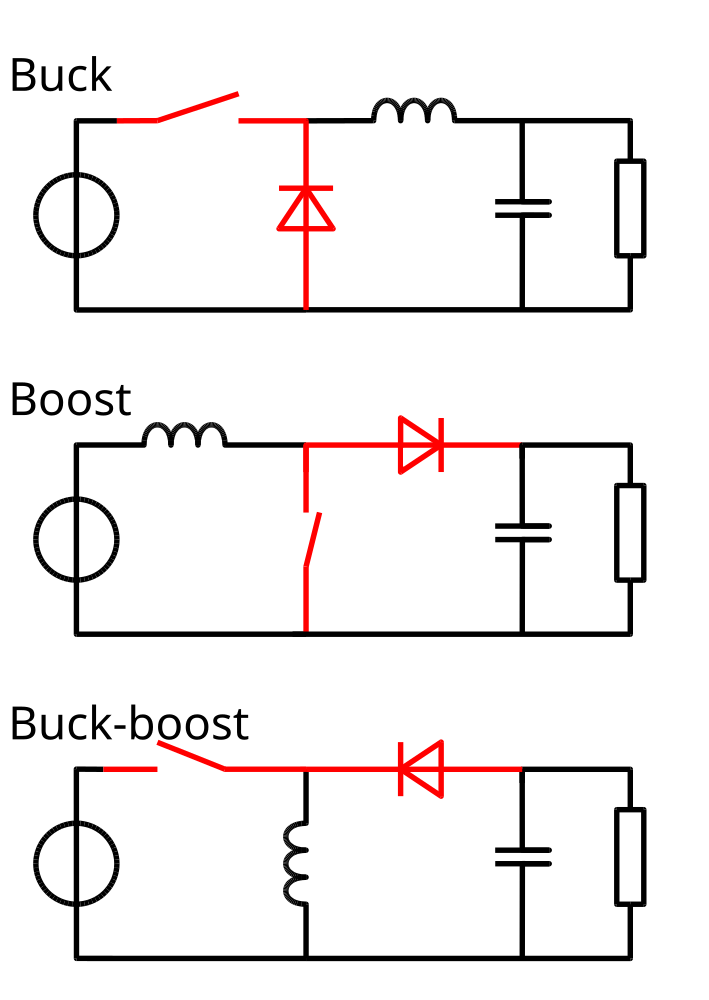
\includegraphics[width = 10cm]{images/przetworniceDC.png}
        \caption{Przetwornice typu buck, boost oraz buck-boost.}
        \label{fig:przetwornice}
    \end{center}
\end{figure}

Istnieją także inne implementacje przetwornic napięciowych, takie jak np.: Ćuk, SEPIC. Ze względu m.in. na ich skomplikowaną konstrukcję (np. stosowanie kondensatora szeregowego), są one dużo mniej popularne od powyżej przedstawionych.
W przypadku konwertera typu buck-boost, należy zauważyć, iż odwraca on napięcie wejściowe, w związku z czym w niektórych przypadkach stosuje się zamiast tego szeregowe połączenie układów buck oraz boost, w celu zachowania polaryzacji napięcia względem wspólnej masy.




\section{Prezentacja problemu}

Przetwornice napięciowe znalazły zastosowanie w znacznej większości urządzeń elektronicznych. Są one stosowane w komputerach, telefonach, zegarkach, urządzeniach medycznych, automatyce, a obecnie nawet w wielu urządzeniach laboratoryjnych i profesjonalnym sprzęcie pomiarowym.
Na stosowanie w tak szerokim zakresie aplikacji, niekiedy bardzo wymagających, pozwolił rozwój półprzewodników, w tym powstanie układów GaN, tranzystorów HEMT i innych, a także integracja niezbędnych elementów przełączających w niewielkich układach scalonych. 
Do dziś, największym problemem pozostają elementy magnetyczne (cewki) oraz kondensatory. W związku z tym, współczesne zasilacze impulsowe pracują z coraz to większymi częstotliwościami przełączania, a co za tym idzie, rosną wymagania co do ich elementów składowych.

Projektanci mają więc do wyboru wiele układów scalonych, elementów przełączających, jak i pasywnych, które należy dobrać odpowiednio do danego zastosowania.
W tym celu, należy znać podstawowe parametry przetwornicy, takie jak:

\begin{itemize}
    \item zakres napięć wejściowych - minimalne oraz maksymalne napięcie wejściowe, dla którego przetwornica utrzymuje zadane napięcie wyjściowe,
    \item regulacja napięcia wyjściowego - zakres zmian napięcia wyjściowego w pełnym zakresie napięć zasilających i dopuszczalnych prądów obciążenia,
    \item sprawność - stosunek mocy wyjściowej do mocy wejściowej, określający jednocześnie ilość mocy wydzielanej przez samą przetwornicę, zgodnie z \ref{eq:1},
    \item poziom szumów wyjściowych - podawany zazwyczaj jako $V_{RMS}$ oraz $V_{peak-peak}$,
    \item fizyczne wymiary układu - ograniczone m.in. pobieraną mocą i częstotliwością przełączania.
\end{itemize}

W zastosowaniach precyzyjnych, takich jak urządzenia pomiarowe, niewątpliwie 
najważniejszą cechą będzie poziom szumów. Jeśli jednak urządzenie zasilane jest 
bateryjnie i wymaga się od niego długiego czasu pracy, konieczne okaże się 
zoptymalizowanie projektu pod kątem sprawności. Niestety, nie jest się  w stanie 
poprawić każdego parametru z osobna, nie wpływając na pozostałe. 

Dzięki rozwojowi technologii, konstruktor może obecnie symulować działanie zasilacza, korzystając z 
oprogramowania takiego jak np. SPICE \cite{spice}. Pozwala to na przewidywanie zachowania 
projektowanego układu jeszcze przed jego skonstruowaniem. Niestety, na parametry 
finalnego produktu wpłynąć mogą elementy pasożytnicze i rozbieżność parametrów modeli 
elementów, które są stosowane. Konieczna jest więc weryfikacja fizycznego układu i jego
pomiary.

Do najpopularniejszych pomiarów należą:

\begin{comment}
W zastosowaniach precyzyjnych, takich jak urządzenia pomiarowe, niewątpliwie najważniejszą cechą będzie poziom szumów. Jeśli jednak nasze urządzenie zasilane jest bateryjnie i wymagamy od niego długiego czasu pracy, konieczne okaże się zoptymalizowanie projektu pod kątem sprawności.
Niestety, nie jesteśmy w  stanie poprawić każdego parametru z osobna, nie wpływając na pozostałe.

Dzięki rozwojowi technologii, jesteśmy obecnie w stanie symulować działanie zasilacza, korzystając z oprogramowania takiego jak np. SPICE \cite{spice}.
Pozwala to na przewidywanie zachowania projektowanego układu jeszcze przed jego skonstruowaniem. Niestety, na parametry finalnego produktu wpłynąć mogą elementy pasożytnicze i rozbieżność parametrów modeli elementów, które stosujemy.
Konieczna jest więc weryfikacja fizycznego układu i jego pomiary. 

Do najpopularniejszych pomiarów należą: 
\end{comment}

\begin{itemize}
    \item pomiar szumów wyjściowych - wykonywany zwykle pod obciążeniem, za pomocą oscyloskopu, bądź analizatora widma,
    \item pomiar regulacji napięcia wyjściowego - wykonywany przy pomocy woltomierza pod obciążeniem,
    \item pomiar sprawności - wymagane jest tu zmierzenie poziomu mocy wejściowej i wyjściowej dla danego obciążenia. 
\end{itemize}

Zdecydowanie najbardziej czasochłonnym z powyższych staje się pomiar sprawności. Jeśli bowiem chcemy zbadać sprawność przetwornicy w szerokim zakresie napięć wejściowych, czy też prądów obciążenia, 
dokonujemy wielu pomiarów, których wynikiem są np. przedstawione tu wykresy \ref{fig:przykladowaSprawnosc}.

\begin{figure}[h!]
    \begin{center}
        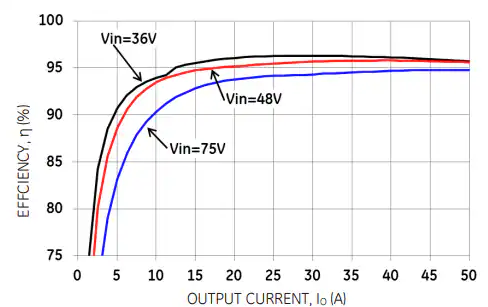
\includegraphics[width = 10cm]{images/przykladowaSprawnosc.png}
        \caption{Przykładowy wykres sprawności przetwornicy w zależności od napięcia wejściowego i prądu obciążenia, źródło: \cite{przetwornicaOmniON}.}
        \label{fig:przykladowaSprawnosc}
    \end{center}
\end{figure}

Do wykonania takiego pomiaru, potrzebne są zazwyczaj:

\begin{itemize}
    \item zasilacz regulowany - zasilający mierzoną przetwornicę,
    \item obciążenie aktywne - pozwalające na zmianę pobieranego z przetwornicy prądu,
    \item dwa woltomierze - do pomiaru napięcia wejściowego i wyjściowego,
    \item dwa amperomierze - do pomiaru prądów wejściowego i wyjściowego.
\end{itemize}

Zakładając, że woltomierze i amperomierze (pomiar mocy) są zintegrowane w układy zasilacza i obciążenia aktywnego, potrzebne są jedynie te dwa urządzenia.
Niestety, często konieczne jest ręczne zapisywanie wyników każdego pomiaru i ponowna zmiana ustawień obu urządzeń, a następnie obróbka otrzymanych danych.

Rozwiązania tego problemu, które mogą skrócić czas i usprawnić proces charakteryzacji przetwornicy, przedstawione zostaną w rozdziale \ref{chapter-2} 
wraz z projektowanym urządzeniem, które integruje niezbędne do wykonania pomiarów elementy.




\chapter{Przegląd obecnych rozwiązań}
\label{chapter-2}

W rozdziale zaprezentowano konstrukcje podobne do realizowanego urządzenia oraz przedstawiono jego ogólną zasadę działania.

\vspace{0.5cm}

\section{Rozwiązania dostępne na rynku komercyjnym}

%Wykonując pomiary przetwornic napięciowych najczęściej korzysta się ze standardowego zasilacza laboratoryjnego oraz obciążenia aktywnego.
%Urządzenia te wymagają jednak często ręcznej zmiany ich ustawień i ręcznego zapisu danych pomiarowych. W celu przyspieszenia tego procesu,
%wielu producentów sprzętu laboratoryjnego umożliwia podłączenie swoich urządzeń do komputera poprzez dedykowany interfejs (LAN, RS232, USB), a następnie
%kontrolę przy pomocy dedykowanej aplikacji, czy też programowanie, np. wykorzysując środowisko LabView. Daje to możliwość stworzenia dedykowanej aplikacji,
%która to mogłaby realizować automatyczne pomiary przetwornic. Wymaga to jednak sporo czasu poświęconego na odpowiednie ustawienie sprzętu, programowanie, a także
%niekiedy wymaga zakupu sprzętu od konkretnego producenta. Należy bowiem zaznaczyć, że nie wszystkie urządzenia tego typu umożliwiają pomiar 
%wszelkich potrzebnych nam parametrów.

Obecnie na rynku możemy znaleźć urządzenia, które integrują w sobie komponenty niezbędne do realizacji omawianego problemu pomiaru parametrów przetwornic.
Za przykład służyć może m.in. N6705C od firmy Keysight \cite{n6705c}, przedstawiony na zdjęciu \ref{fig:N6705C}.

\begin{figure}[h!]
    \centering
 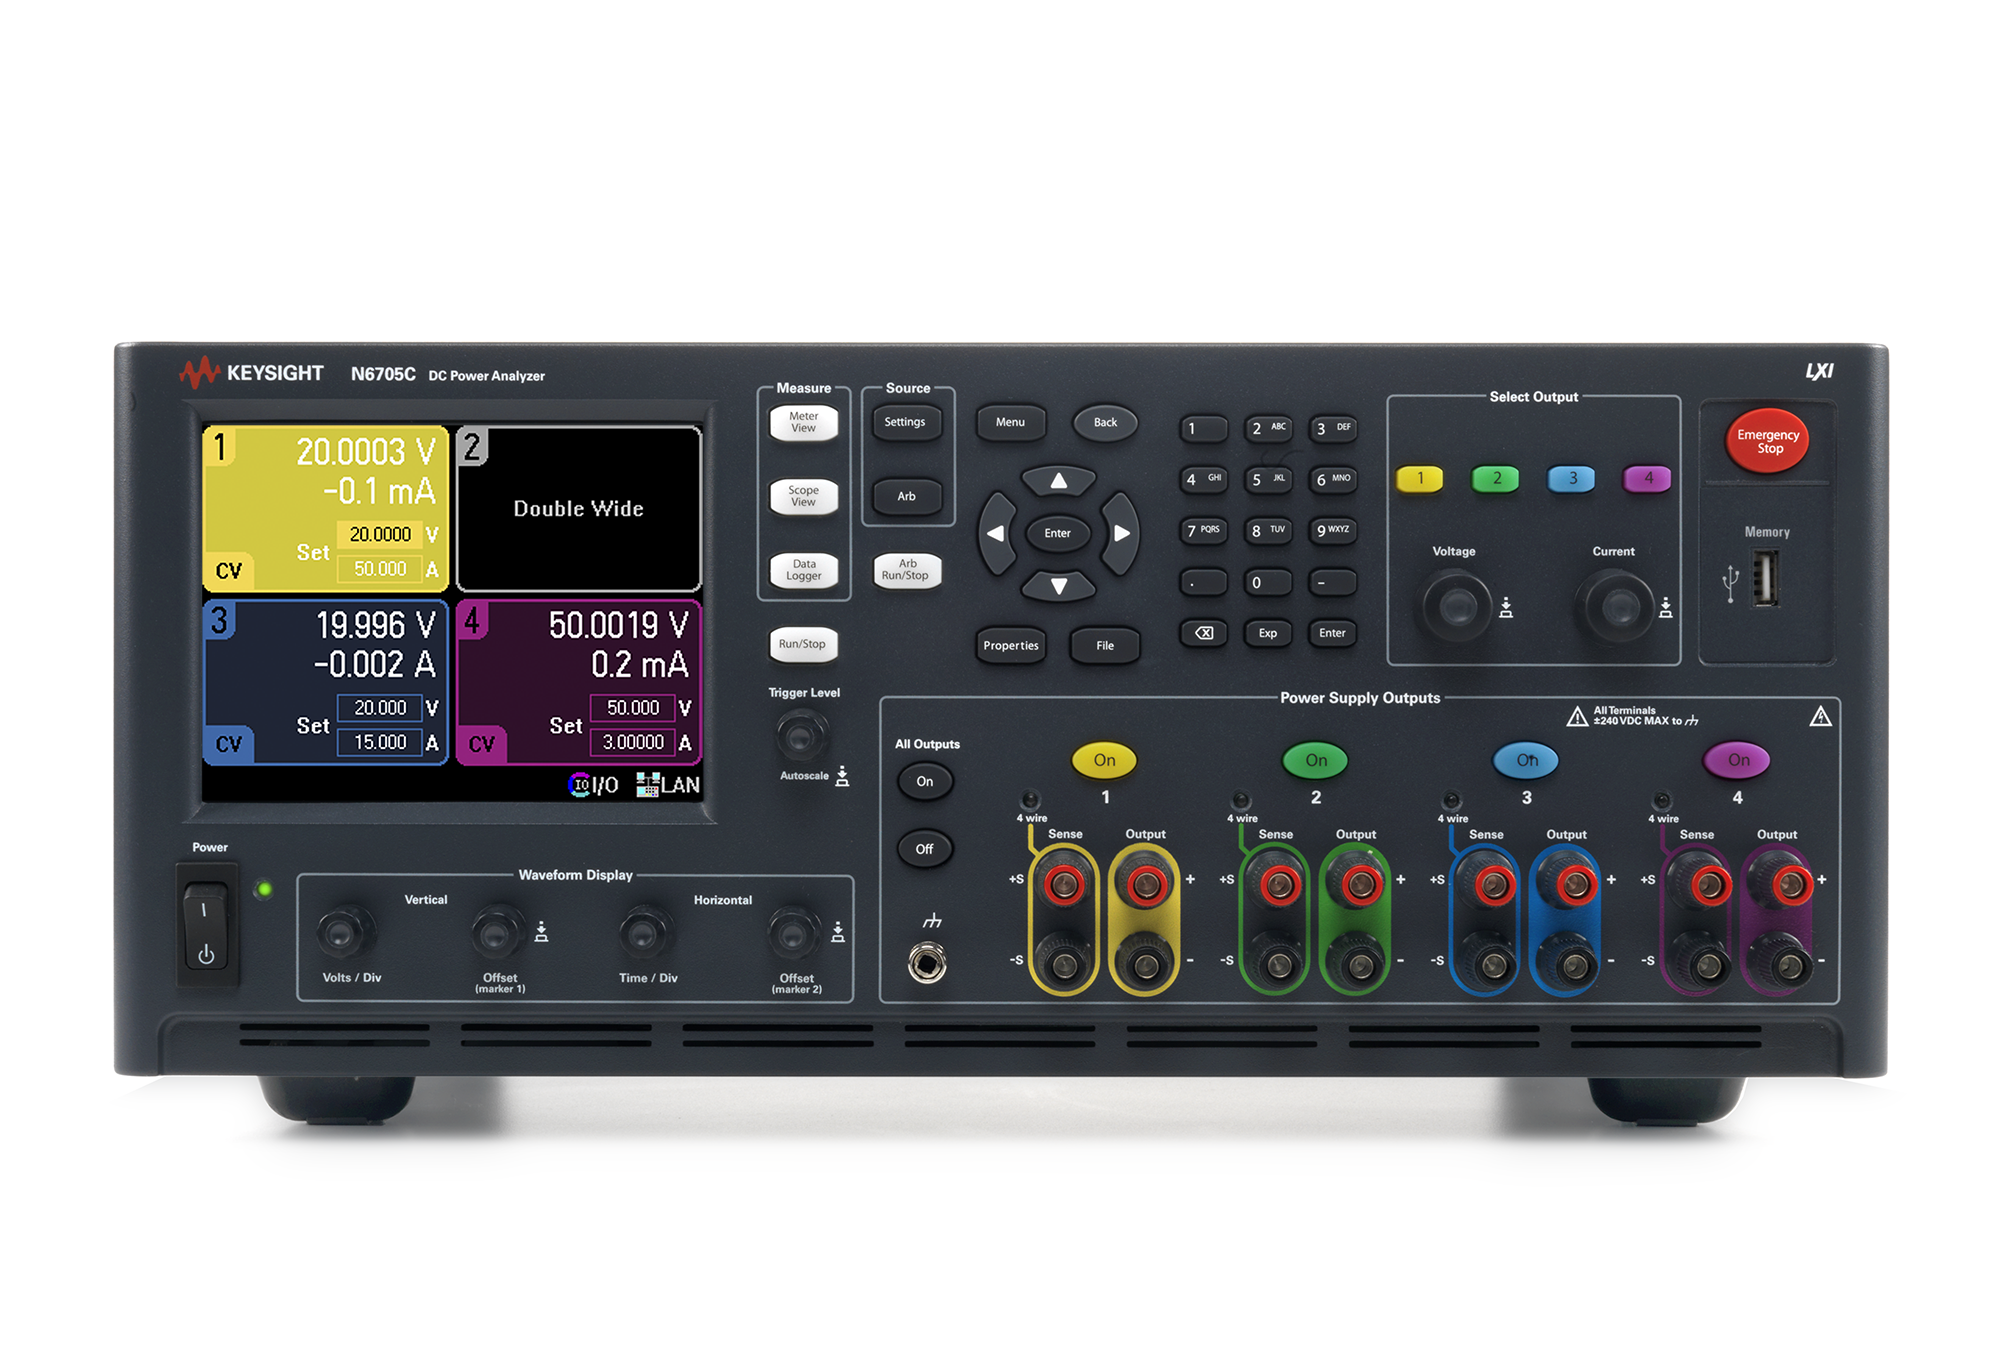
\includegraphics[width = 15cm]{images/n6705c.png}
 \caption{N67005C firmy Keysight.}
 \label{fig:N6705C}
\end{figure}

Przedstawione urządzenie posiada funkcje oscyloskopu, precyzyjnego woltomierza, miernika prądu, generatora funkcyjnego oraz logowania danych.

Kolejną opcję stanowią tzw. Bidirectional Power Supplies, jak np. te od firmy ElektroAutmatik \cite{bidirectional_DC_PSU}. 
Poniżej \ref{fig:ElektroAutomatik} widoczne jest jedno z takich urządzeń.


\begin{figure}[h!]
    \centering
 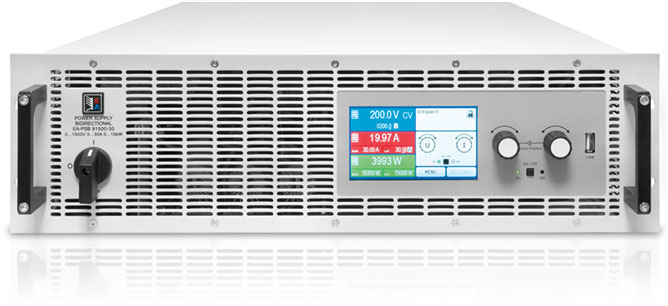
\includegraphics[width = 15cm]{images/elektroautomatik.jpg}
 \caption{Przykładowy zasilacz dwukierunkowy od ElektroAutmatik.}
 \label{fig:ElektroAutomatik}
\end{figure}

Takie przyrządy integrują w sobie zasilacze DC - najczęściej przetwornice impulsowe o dużej mocy - oraz obciążenie aktywne.
Pozwala to na pomiar mocy wyjściowej i wejściowej. Znaleźć można urządzenia tego typu od różnych producentów, różniące się parametrami, obudową (w tym przypadku typu rack), czy też interfejsami komunikacyjnymi.

Cechą wspólną obu zaprezentowanych rozwiązań jest niestety ich wysoka cena. Są to narzędzia dla specjalistów, mające wąski zakres zastosowań, w związku z czym ciężko jest znaleźć podobne instrumenty w budżecie kilku lub kilkunastu tysięcy złotych.
Kolejną wadą może okazać się brak możliwości modyfikacji, zarówno sprzętu, jak i oprogramowania. Użytkownik nie ma pełnej kontroli nad działaniem swojego sprzętu, co w niektórych wypadkach utrudnia przeprowadzenie wymaganych testów, bądź pomiarów.



%Na rynku powstały już zintegrowane urządzenia, zawierające w sobie niezbędne komponenty, takie jak zasilacz regulowany i obciążenie aktywne.
%Przykładem jest tu N6705C od firmy Keysight [TODO: DODAĆ ZDJĘCIA + REFERENCJA DO ŹRÓDŁA (https://www.keysight.com/us/en/product/N6705C/dc-power-analyzer-modular-600-w-4-slots.html)]
%Urządzenie to pozwala na wykonywanie pomiaru sprawności przetwornic napięciowych i przesłanie danych do komputera w celu dalszej ich analizy.
%Wadą takiego rozwiązania jest jednak cena przedstawionego urządzenia, a także zamknięte oprogramowanie, które nie pozwala na wprowadzanie własnych modyfikacji.
%Zamyka to możliwość na samodzielne rozszerzanie funkcjonalności takiego produktu.
%...

\section{Alternatywne rozwiązania}

Chcąc pozbyć się problemu ceny oraz braku możliwości dostosowywania urządzeń do wymagań użytkownika, inżynier może zdecydować się na zbudowanie własnego stanowiska testowego, służącego pomiarowi parametrów przetwornic napięciowych.
Jak już wspomniano, w tym celu można wykorzystać zasilacz regulowany, obciążenie aktywne, woltomierze, amperomierze, oscyloskop (np. do pomiaru szumów wyjściowych).
Aby usprawnić proces testowania, tego typu instrumenty posiadają często interfejsy komunikacyjne, takie jak: RS232, RS485, Ethernet, USB.
Umożliwia to podłączenie do komputera i zdalne sterowanie parametrami tych instrumentów. W zależności od producenta, dokonuje się tego poprzez dedykowaną aplikację, interfejs webowy albo odpowiednie API.
Przykładowymi językami programowania, które można wykorzystać do kontroli stanowiska testowego są Python \cite{python} i LabView \cite{labview}.

Najczęściej wybieranym środowiskiem do tego typu zastosowań pozostaje LabView. Na rysunku \ref{fig:labview_grafika} przedstawiony został przykładowy interfejs użytkownika stworzony przy jego pomocy.

\begin{figure}[h!]
 \centering
 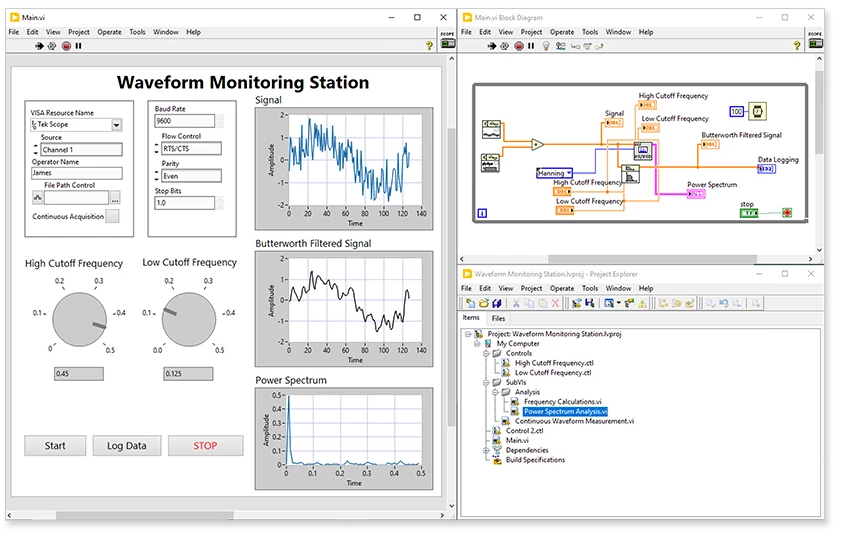
\includegraphics[width = 15cm]{images/labview.png}
 \caption{Przykładowy interfejs stworzony przy pomocy LabView.} 
 \label{fig:labview_grafika}
\end{figure}

Do niewątpliwych zalet takiego rozwiązania należy zaliczyć możliwość wykorzystania posiadanego już sprzętu, a także łatwość rozbudowy i przystosowania do innego typu pomiarów.
Niestety, może się okazać, że wykorzystywane instrumenty nie posiadają łatwo dostępnego API, które umożliwiałoby integrację. Nierzadko przeszkodę stanowi także samo środowisko, do którego użycia niejako zmusza producent.

%\chapter{Proponowane rozwiązanie}
\section{Proponowane rozwiązanie}
%\label{chapter-3}

\vspace{0.5cm}

\begin{comment}
Celem projektu było zaprojektowanie i skonstruowanie urządzenia umożliwiającego pomiar parametrów przetwornic napięciowych DC/DC, które przedstawione zostały w rozdziale \ref{chapter-2}.

Urządzenie takie powinno posiadać następujące właściwości:
\begin{itemize}
    \item Możliwość pomiaru sprawności przetwornic, regulacji napięcia wyjściowego, zakresu napięć wejściowych i prądów obciążenia.
    \item Modularność konstrukcji
    \item Możliwość dodania kolejnych modułów, umożliwiających wykonywanie innych pomiarów.
    \item Łatwość modyfikacji sprzętu i oprogramowania.    
    \item Niska cena w porównaniu do rozwiązań komercyjnych.
\end{itemize}

W celu spełnienia przedstawionych powyżej założeń, zaprojektowane urządzenie musi posiadać:
\begin{itemize}
    \item zintegrowany zasilacz regulowany
    \item zintegrowane obciążenie aktywne
    \item wbudowany kontroler, pozwalający na pracę bez konieczności podłączania do komputera, wyposażony w podstawowy interfejs użytkownika z wyświetlaczem
\end{itemize}

Elementy te zostały przedstawione na schemacie blokowym \ref{fig:schematBlokowy}.

\begin{figure}[h!]
    \begin{center}
        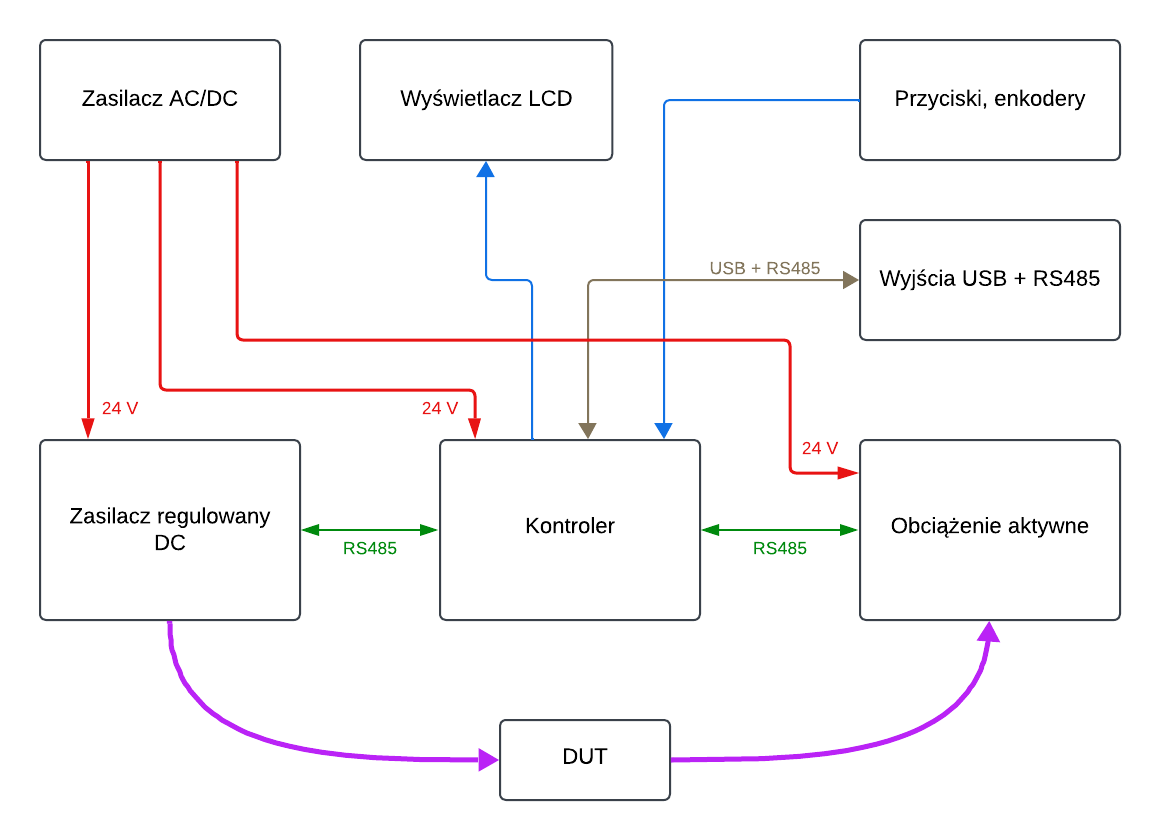
\includegraphics[width = 17cm]{images/schemat_blokowy.png}
        \caption{Schemat blokowy urządzenia.}
        \label{fig:schematBlokowy}
    \end{center}
\end{figure}

\end{comment}

Proponowane rozwiązanie zakłada projekt trzech modułów: kontrolera, obciążenia aktywnego i zasilacza regulowanego, 
które komunikują się między sobą przy pomocy odpowiedniego interfejsu.
Elementy te zostały przedstawione na schemacie blokowym \ref{fig:schematBlokowy}.
W celu umożliwienia użytkownikowi sterowania poszczególnymi modułami, urządzenie musi posiadać duży i czytelny wyświetlacz, a także panel frontowy z przyciskami i enkoderami.
Dodatkowe złącza USB oraz RS485 mają na celu umożliwienie sterowania poprzez komputer lub inne urządzenie laboratoryjne.
Za zasilanie wszystkich modułów odpowiada zasilacz, przekształcający napięcie sieciowe 230V AC na 24V DC, co pozwala uniknąć projektowania dedykowanych zasilaczy sieciowych dla każdego modułu.

Kolejnym ważnym aspektem jest zakres napięć i prądów, jakie dostarczyć należy do testowanej przetwornicy, oznaczonej na schemacie jako DUT
 (ang. \textit{Device Under Test}).
Zdecydowano się na zakres napięć wyjściowych 0-20 V i prąd do 2 A dla zasilacza regulowanego, jak również 0-20 V dla napięć wejściowych obciążenia aktywnego, z maksymalnym prądem 2A, co daje maksymalną wydzielaną moc na poziomie 40W.
Zdaniem autora, jest to zakres wystarczająco szeroki do testowania większości przetwornic, jakie stosowane są w wielu urządzeniach.
Zakłada to bowiem możliwość testowania przetwornic pracujących z napięciami: 3.3V, 5V, 9V, 12V, 15V, 20V, które znaleźć można np. w USB Power Delivery, a także
przetwarzających napięcie z akumulatorów LiIon, LiPo, lead-acid, LiFePO4.

Jak łatwo zauważyć, urządzenie takie umożliwia nie tylko pomiar parametrów przetwornic. Zasilacz regulowany oraz obciążenie aktywne mogą też być wykorzystywane oddzielnie,
zasilając inne urządzenia elektroniczne, dokonując pomiarów napięć i poboru prądu. 
Do mniej oczywistych zastosowań zaliczyć można pomiar pojemności baterii, mierząc ich ładowanie i rozładowanie, pomiar rezystancji przewodów, a co za tym idzie także ich długości, czy też automatyzacja pomiarów dokonywanych przez
inne sprzęty laboratoryjne, co można uzyskać podłączając je do wyprowadzeń kontrolera.

Znając już założenia projektu pod kątem elektrycznym, należy się skoncentrować nad aspektem mechanicznym urządzenia.
W celu uzyskania modularnej konstrukcji, która umożliwi dalszą rozbudowę, zdecydowano się ujednolicić konstrukcję poszczególnych modułów. 
Każdy z nich posiada PCB o wymiarach 150x100 mm. Wejściowe napięcie zasilające to 24V DC. Komunikacja natomiast odbywa się poprzez interfejs RS485. 

Szczegółowe rozwiązania układowe zostaly przedstawione w rozdziale \ref{chapter-4}, gdzie prezentowany jest zarówno projekt elektroniki, jak i obudowy i okablowania.

\begin{figure}[h!]
    \begin{center}
        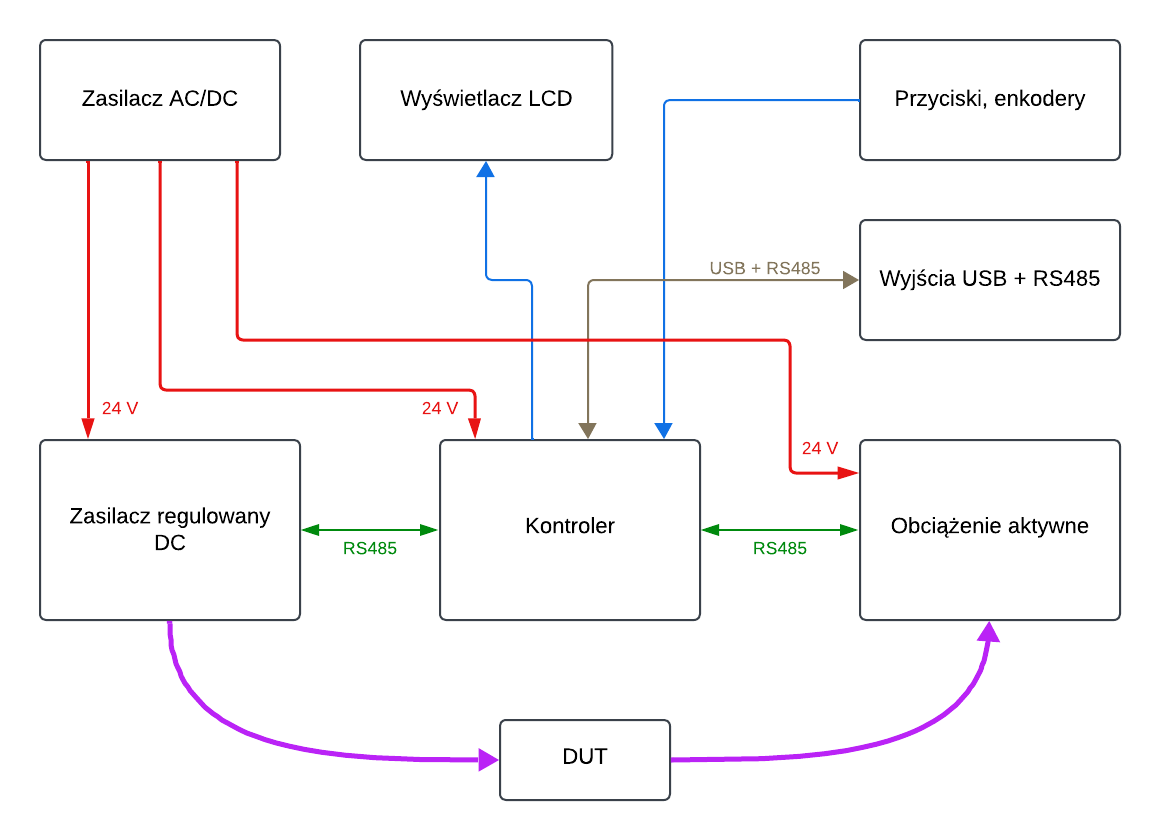
\includegraphics[width = 17cm]{images/schemat_blokowy.png}
        \caption{Schemat blokowy urządzenia.}
        \label{fig:schematBlokowy}
    \end{center}
\end{figure}










\chapter{Realizacja projektu}
\label{chapter-4}


\vspace{0.5cm}


W tym rozdziale opisany został proces projektowania zarówno elektroniki, jak i elementów mechanicznych, a także tworzenia oprogramowania urządzenia.


\section{Projekt elektroniki}

Projekt elektroniki podzielony został na poszczególne moduły, które zostały opisane szczegółowo w kolejnych rozdziałach. 
Aby przyspieszyć proces projektowania oraz zapewnić kompatybilność między modułami, niektóre podukłady wykorzystywane są we wszystkich trzech modułach. 
Z uwagi na stopień rozbudowania projektów, nie przedstawiono tu wszystkich schematów elektronicznych oraz projektów PCB, a jedynie najważniejsze omawiane fragmenty. Można je natomiast znaleźć w załączniku.

Przedstawione tu schematy elektroniczne oraz projekty płytek PCB powstały przy pomocy oprogramowania Altium Designer \cite{altiumDesigner}, korzystając z licencji studenckiej AGH.


\subsection{Kontroler}

W tej sekcji przedstawiono projekt kontrolera - modułu, który umożliwia sterowanie zasilaczem regulowanym, obciążeniem aktywnym i potencjalnie innymi urządzeniami.

\subsubsection{Schemat blokowy}

Rysunek \ref{fig:schematBlokowyKontrolera} przedstawia schemat blokowy modułu kontrolera, na którym widoczne są wszystkie jego podstawowe bloki składowe.

\begin{figure}[h!]
    \begin{center}
        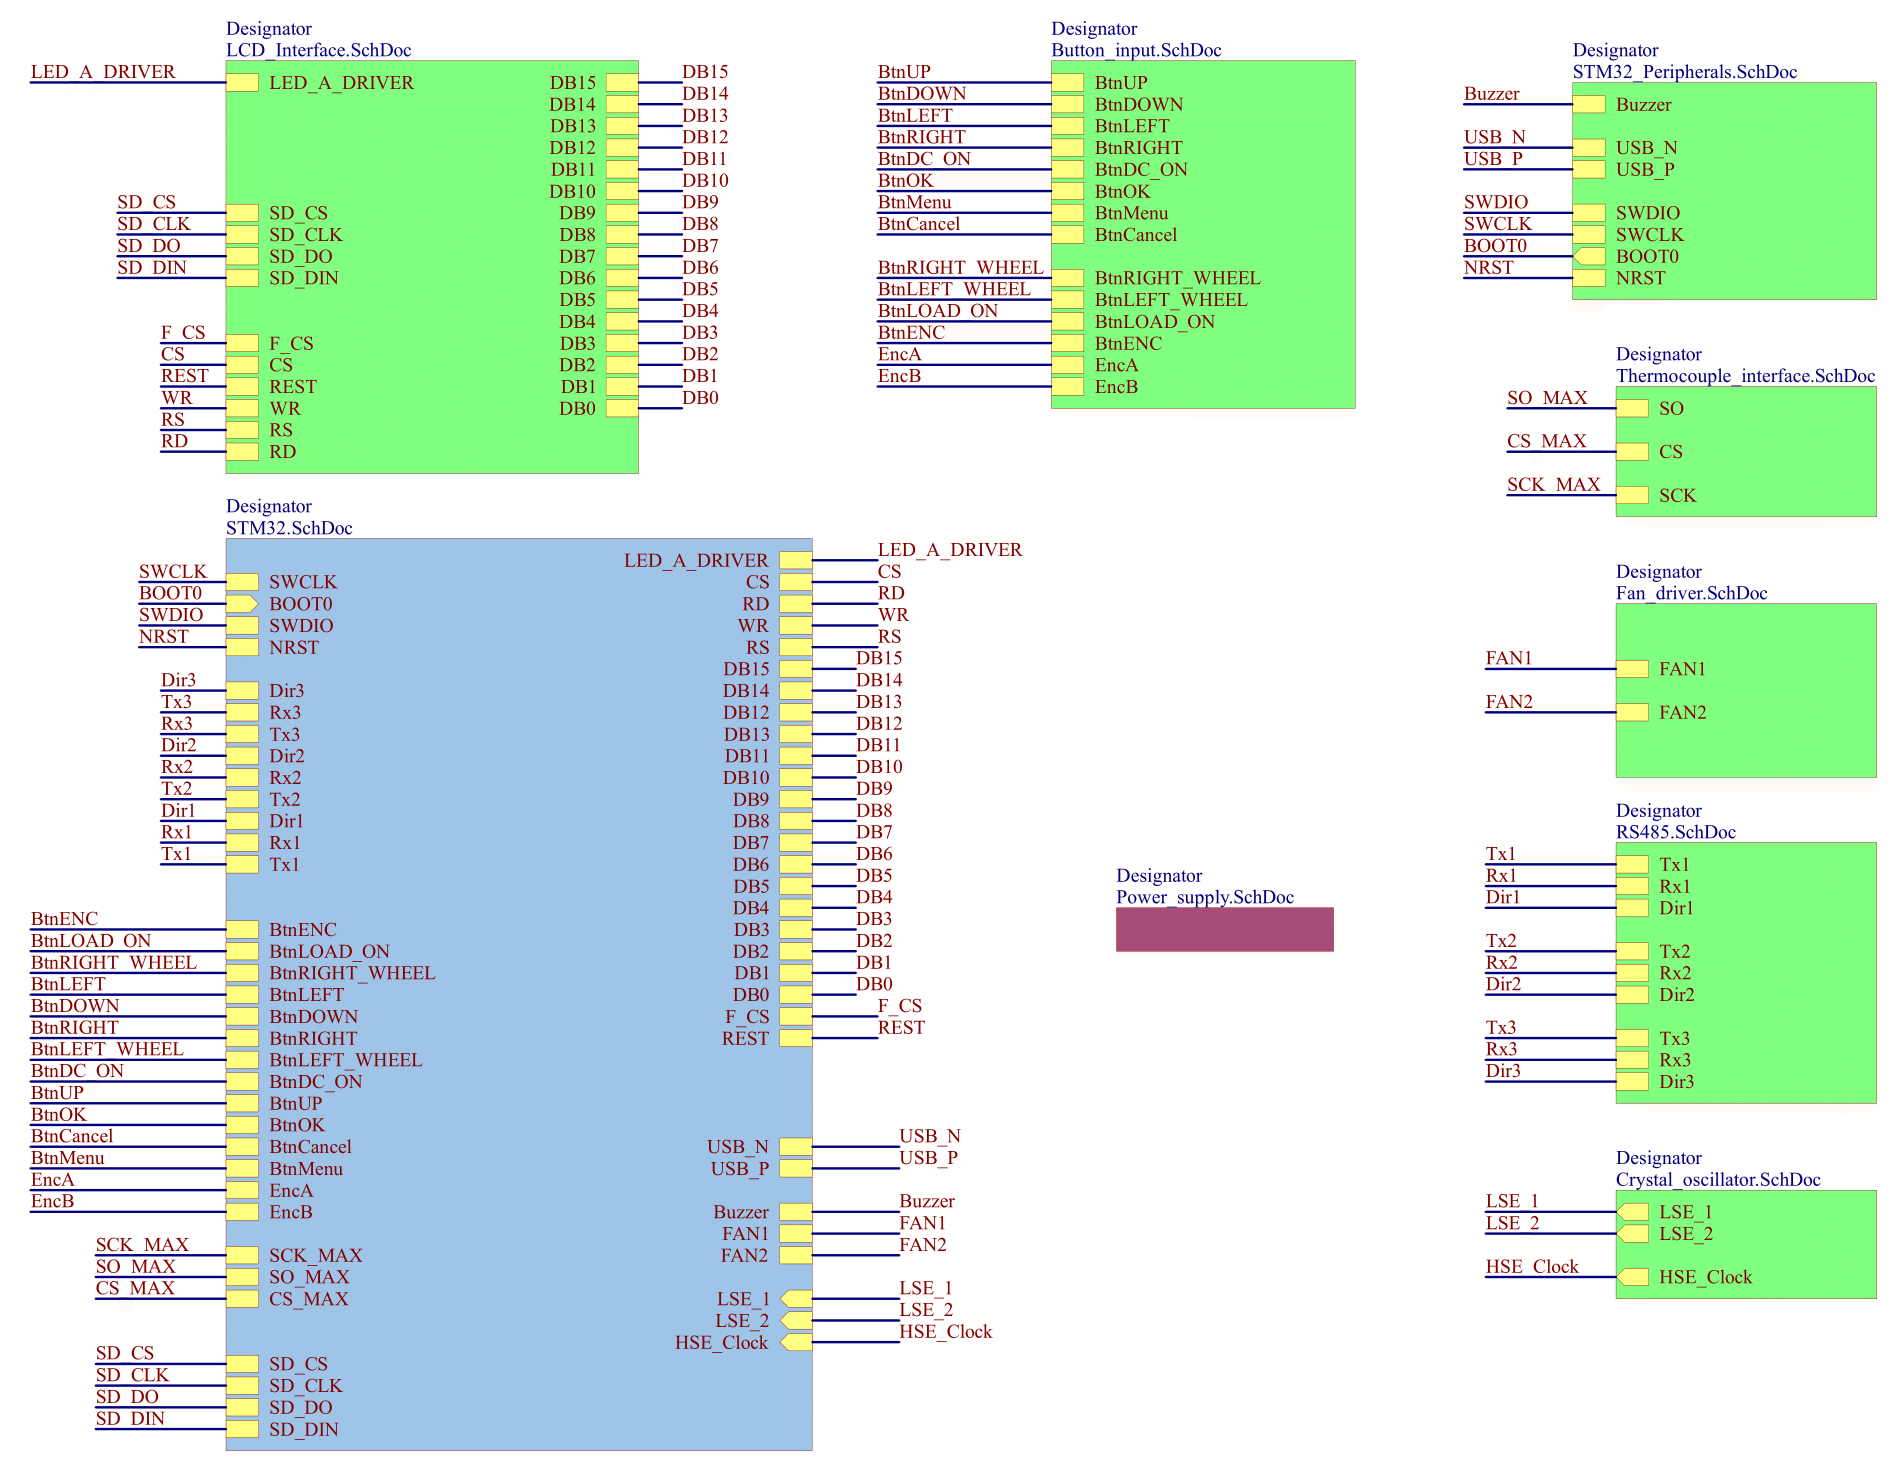
\includegraphics[width = 17cm]{images/schemat_blokowy_kontrolera_2.png}
        \caption{Schemat blokowy modułu kontrolera.}
        \label{fig:schematBlokowyKontrolera}
    \end{center}
\end{figure}

Centralnym elementem układu jest mikrokontroler omówiony w następnej sekcji. 
Oprócz niego, znajduje się tu interfejs wyświetlacza LCD, złącza umożliwiające podłączenie przycisków oraz enkoderów, złącze termopary z dedykowanym układem, kontroler wentylatorów,
interfejsy RS485, a także inne układy peryferyjne. 

\subsubsection{Sekcja mikrokontrolera}

Wybranym do modułu kontrolera mikrokontrolerem jest STM32F401VET6 \cite{stm32f401}. Jest to układ oparty o 
32-bitowy rdzeń ARM Cortex M4, taktowany maksymalną częstotliwością 84MHz. W wybranej wersji posiada on 
512kB pamięci typu Flash oraz 96kB pamięci podręcznej RAM. Wśród jego interfejsów znajdują się: UART, I2C, SPI, wbudowany kontroler USB 2.0 full-speed. Możliwe jest również 
skorzystanie z wbudowanego układu RTC (Real Time Clock). Wyjścia / wejścia układu mogą być taktowane z częstotliwością aż 42MHz, co okazało się ważne podczas podłączania wyświetlacza poprzez interfejs równoległy.

Kluczowymi aspektami przy wyborze mikrokontrolera była wielkość pamięci wbudowanej, dostępność wymaganych interfejsów, szybkość działania, a także łatwość programowania.
Mikrokontrolery z serii STM32 posiadają bowiem liczne biblioteki do obsługi popularnych układów peryferyjnych, co wraz z oprogramowaniem STM32CubeMX pozwala na szybkie testowanie i łatwą modyfikację oprogramowania.

Wśród załączonych schematów, STM32F401 znajduje się na stronie zatytułowanej "Moduł kontrolera: STM32".
Oprócz niego, na stronie tej widać niezbędne do prawidłowej pracy kondensatory filtrujące zasilanie, oddzielnie dla linii VDD, VDDA, a także wbudowanych regulatorów, podpięte pod wyprowadzenia VCAP\_1, VCAP\_2, zgodnie z zaleceniami producenta
zawartymi w datasheet \cite{stm32f401}.	



\subsubsection{Komunikacja RS485}

Do komunikacji z pozostałymi modułami wybrany został interfejs RS485, obecnie nazywany EIA-485 \cite{RS485}.
Standard RS485 składa się z pary różnicowej, nie ma konieczności podłączania sygnału zwrotnego, jednak w niektórych przypadkach może to poprawić jakość transmisji.
Umożliwia ona podłączenie do 32 układów nadajnika / odbiornika, a najczęściej stosowaną topologią podłączenia jest magistrala (szyna).

Standard definiuje parę różnicową, jako dwie linie, oznaczone odpowiednio A oraz B. Jeśli na linii A, napięcie jest mniejsze od napięcia na linii B, odczytywane jest to jako logiczna jedynka (1). W przeciwnym wypadku, występuje logiczne zero (0).
Maksymalne dopuszczalne wspólne obu linii może wahać się w zakresie od -7V do +12V, a napięcia różnicowe są z zakresu 0V do 5V. Przykład
komunikacji przedstawiony jest na rysunku \ref{fig:poziomyNapiecRS}.

\begin{figure}[h!]
    \begin{center}
        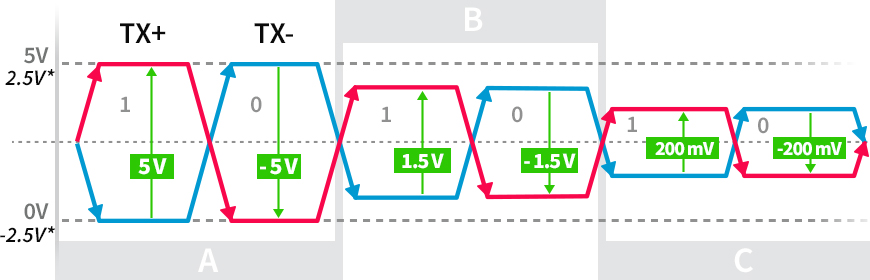
\includegraphics[width = 17cm]{images/rs485_voltages.jpg}
        \caption{Poziomy napięć w standardzie RS485, źródło \cite{napieciaRS}.}
        \label{fig:poziomyNapiecRS}
    \end{center}
\end{figure}


W modułach kontrolera, zasilacza regulowanego, a także obciążenia aktywnego, zastosowano układ nadajnika / odbiornika RS-485, oparty o układ MAX3485 (rysunek  \ref{fig:schematRS485}). Jest to wersja 
bardzo popularnego transceivera MAX485, przystosowana do pracy z napięciem zasilającym 3.3V.
\begin{comment} 
Został on przedstawiony na rysnku \ref{fig:schematRS485}, przedstawiającym fragment schematu.
\end{comment}

\begin{figure}[h!]
    \begin{center}
        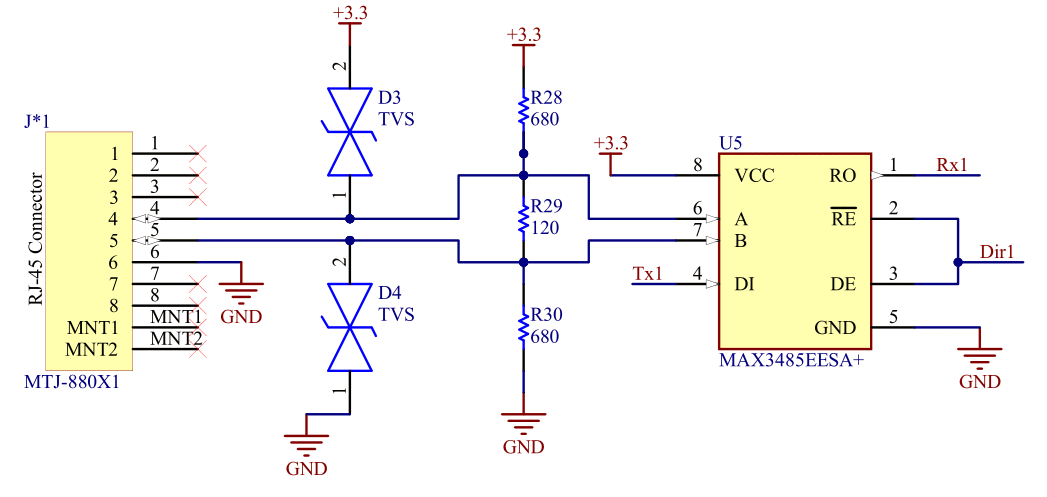
\includegraphics[width = 17cm]{images/schematrs485_3.png}
        \caption{Schemat zastosowanego układu transceivera RS485.}
        \label{fig:schematRS485}
    \end{center}
\end{figure}

Do wyprowadzeń A oraz B układu MAX3485 \cite{MAX3485} podłączone zostały rezystory terminujące o wartościach 680$\Omega$ oraz 120$\Omega$.
Rezystory te odpowiadają za ustawienie biasu na liniach, a także zapobiegają odbiciom, będąc dopasowane do impedancji charakterystycznej linii transmisyjnej (standardowo 120$\Omega$ dla pary skrętki).

Przy konektorze znalazło się również miejsce na diody TVS (Transient Voltage Supression), stanowiące ochronę przed przepięciami na liniach magistrali.

Do popularnych złącz wykorzystywanych do interfejsów RS485 i RS422 należą złącza DB-9, bądź złącza śrubowe. W tym przypadku zdecydowano się jednak 
na rozwiązanie oparte o złącza RJ45, na których wyprowadzono również masę (GND). Dzięki podłączeniu linii A i B do pinów 4 i 5 złącza, możliwe jest wykorzystanie klasycznych kabli 
o postaci skrętki, np. patchcord, mając pewność, że połączenie będzie działać niezależnie od wykorzystywanego standardu okablowania.

Układ MAX3485 konwertuje sygnały odebrane poprzez interfejs wejściowy na UART ($Rx$, $Tx$). Z uwagi na fakt, że standard ten, w przeciwieństwie do RS422, obsługuje
komunikację typu half-duplex, konieczne jest jeszcze wybranie kierunku komunikacji poprzez wyprowadzenia $\overline{RE}$ i $DE$.




\subsubsection{Wyświetlacz LCD}

Wybór wyświetlacza podyktowany był przede wszystkim rozmiarem, rozdzielczością i ceną. Ostatecznie zdecydowano się na moduł 
7" LCD o rozdzielczości 800x480 px z wbudowanym kontrolerem SSD1963 \cite{SSD1963}. 

Kontroler SSD1963 daje możliwość sterowania matrycami LCD, o rozdzielczości do 864x480 px, poprzez interfejs równoległy o 
szerokości 8/9/16/18/24-bitów. Ma wbudowany bufor o pojemności 1215kB i wsparcie dla m.in. sprzętowego obracania obrazu.

Poniższy schemat (\ref{fig:schematWyswietlacz}) przedstawia złącze wykorzystywane do komunikacji z modułem wyświetlacza. Jest to złącze szpilkowe o rastrze 2.54 mm, dokładnie takie samo jak 
występujące na zastosowanym wyświetlaczu. Dzięki temu możliwe jest połączenie między nimi przy pomocy 40-pinowej taśmy IDC.
Na złączu poza pinami od kontrolera SSD1963 widać także piny od złącza karty SD, które znajduje się na płytce wraz z wyświetlaczem. 
Sam wyświetlacz wymaga zasilania 3.3V oraz 5V.

\begin{figure}[h!]
    \begin{center}
        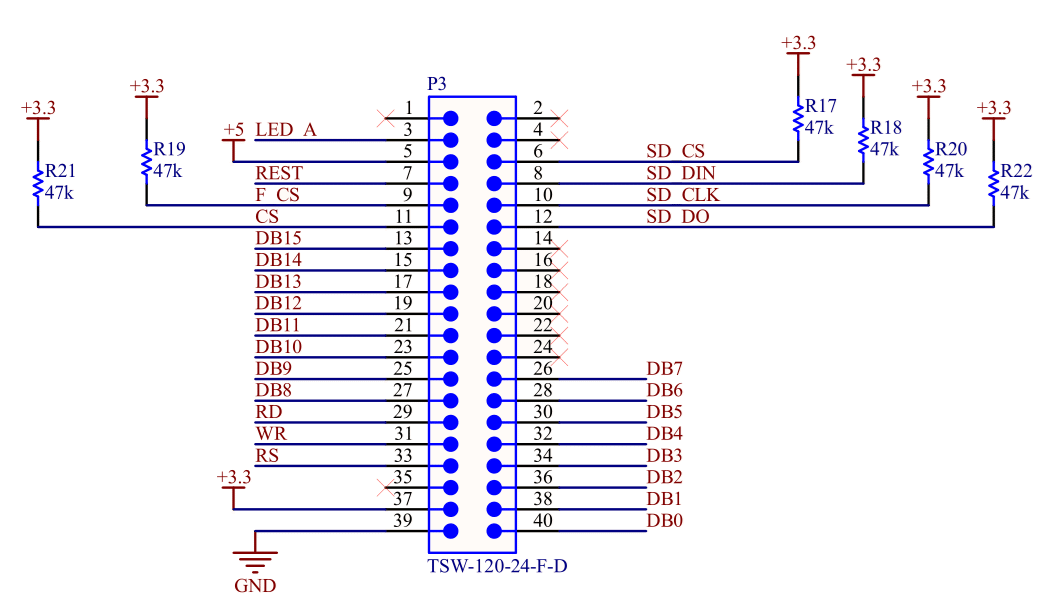
\includegraphics[width = 17cm]{images/schematwyswietlacz_2.png}
        \caption{Schemat złącza wyświetlacza.}
        \label{fig:schematWyswietlacz}
    \end{center}
\end{figure}

Dodatkowo możliwe jest sterowanie podświetleniem matrycy poprzez pin LED\_A. W celu regulacji podświetlenia z poziomu mikrokontrolera 
zdecydowano się na realizację poniższego układu sterowania podświetleniem (\ref{fig:sterowaniePodswietleniem}).

\begin{figure}[h!]
    \begin{center}
        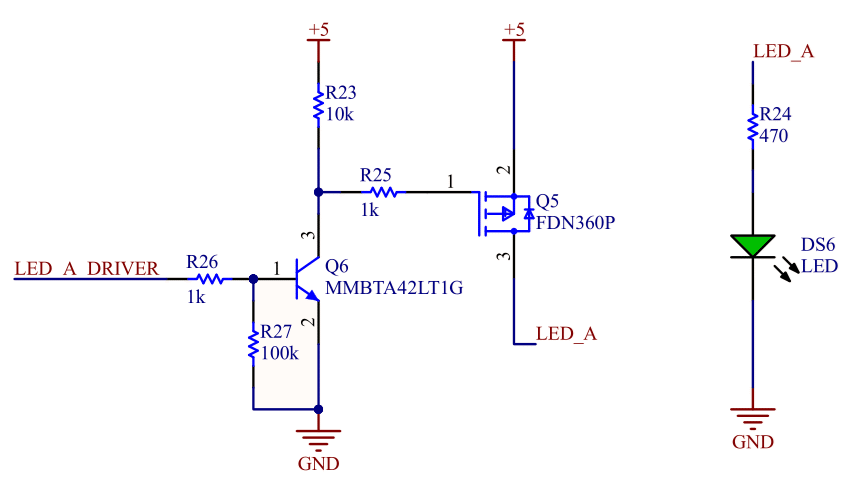
\includegraphics[width = 17cm]{images/sterowaniePodswietleniem_2.png}
        \caption{Schemat sterowania podświetleniem matrycy LCD.}
        \label{fig:sterowaniePodswietleniem}
    \end{center}
\end{figure}

Zastosowanie dodatkowego tranzystora typu NPN (oznaczonego na schemacie jako Q6) pozwala na przełączanie napięcia 5V poprzez piny GPIO mikrokontrolera, pracujące z napięciem VDD (3.3V).



\subsubsection{Interfejs użytkownika}

Do sterowania urządzeniem przez użytkownika służą oddzielne płytki PCB, 
posiadające przyciski i enkoder. Za ich pomocą możliwa jest zmiana opcji 
menu programu, ustawień poszczególnych pozycji menu i konfiguracja kontrolera. 
Na płytkach, poza przyciskami, znalazły się również filtry RC, mające na celu
wytłumienie drgań styków (debouncing). Ich schematy zamieszczone zostały w 
załączniku. Łączą się one z modułem kontrolera przy pomocy 10-pinowych 
taśm IDC.

Modele 3D PCB zostały przedstawione na poniższym zdjęciu \ref{fig:modeleprzyciskow}.

\begin{figure}[h!]
    \begin{center}
        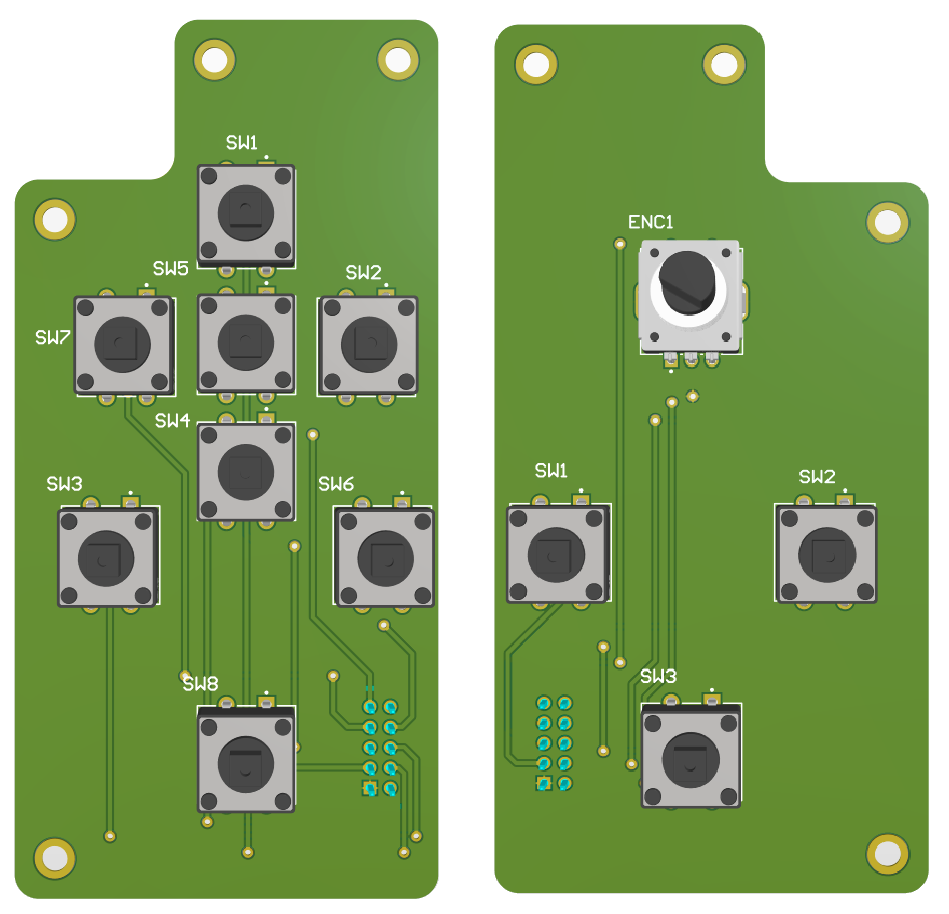
\includegraphics[width = 13cm]{images/modele_przyciskow.png}
        \caption{Modele PCB z przyciskami i enkoderem w programie Altium Designer.}
        \label{fig:modeleprzyciskow}
    \end{center}
\end{figure}




\subsubsection{Termopara}

Podczas pomiaru przetwornic napięciowych, wydzielać może się w nich znaczna ilość ciepła. Jest to wynik strat w układzie, które objawiać się mogą postępującą degradacją 
parametrów przetwornicy. Możliwe jest również przegrzanie elementów przełączających, takich jak diody i tranzystory. Dlatego też, 
zdecydowano się umożliwić pomiar temperatury poszczególnych komponentów, wykorzystując w tym celu termoparę \cite{termopara}.

\begin{figure}[h!]
    \begin{center}
        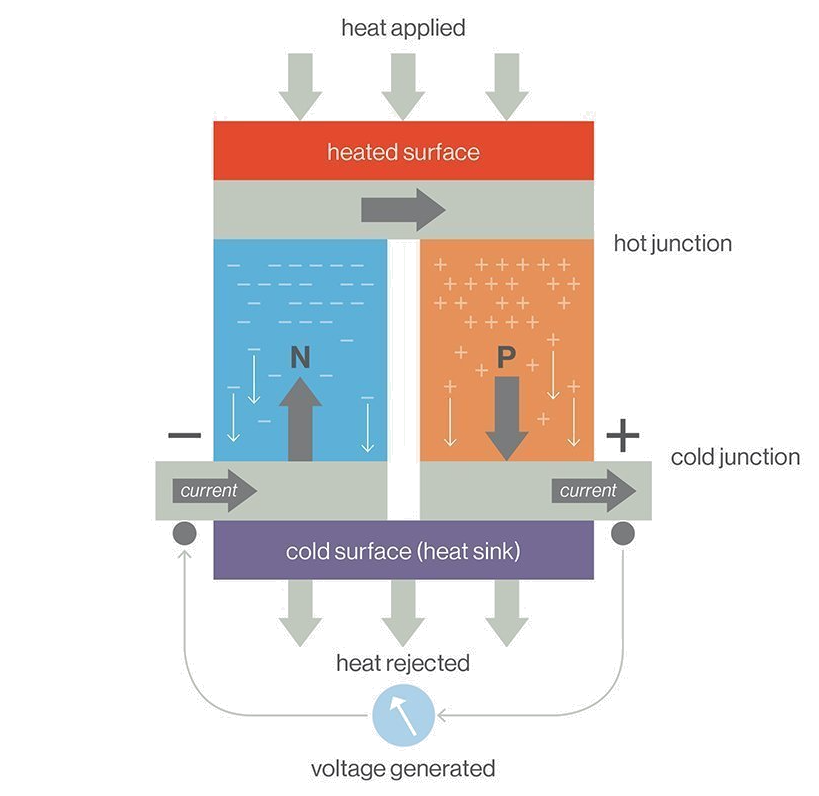
\includegraphics[width = 13cm]{images/thermocouple_2.jpg}
        \caption{Zjawisko Seebecka wykorzystywane w termoparze, źródło \cite{termoparaSeebeck}.}
        \label{fig:thermocouple}
    \end{center}
\end{figure}

Termopara jest to element składający się z dwóch różnych przewodników, na których styku występuje zjawisko Seebecka (rysunek \ref{fig:thermocouple}). Objawia się ono wytworzeniem napięcia na przewodnikach, czyli przewodach termopary.
Napięcie to zależy od typu termopary, czyli zastosowanych materiałów. W celu pomiaru temperatury, wykorzystywany jest układ przetwornika ADC mierzący napięcie na złączu termopary.
Wymagana jest również kompensacja tzw. zimnego końca, tzn. znajomość temperatury w jakiej znajduje się układ pomiarowy, podłączony do przewodów termopary.

W celu uproszczenia pomiaru powstały gotowe układy scalone, posiadające wbudowane przetworniki, układ kompensujący i linearyzujący, mogące cyfrowo przesłać mierzoną temperaturę.
W projekcie zdecydowano się na wykorzystanie układu MAX6675 do termopar typu K \cite{max6675}.

Ten prosty układ, widoczny na schemacie \ref{fig:max6675schemat}, umożliwia odczytanie temperatury przez mikrokontroler poprzez
prosty interfejs SPI.

\begin{figure}[h!]
    \begin{center}
        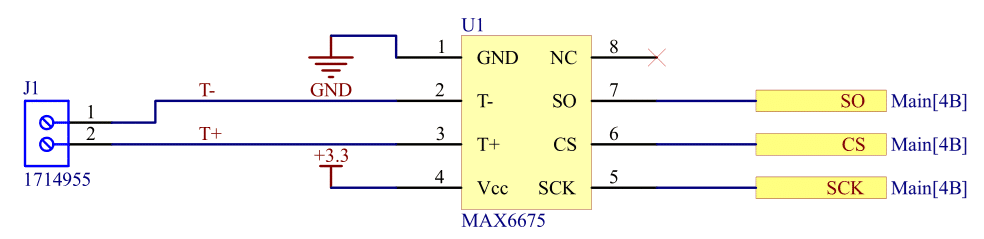
\includegraphics[width = 17cm]{images/max6675_3.png}
        \caption{Układ MAX6675 do pomiaru temperatury.}
        \label{fig:max6675schemat}
    \end{center}
\end{figure}








\subsubsection{Zasilanie}


Do każdego modułu dostarczone jest zasilane 24V DC. Przedstawione w tym rozdziale układy potrzebują jednak również napięć zasilających 5V oraz 3.3V, przy czym 
wyświetlacz wymaga odpowiednio 400mA prądu na linii 5V oraz 200mA na linii 3.3V. Głównie z tego względu, nie ma możliwości zastosowania regulatora liniowego do obniżenia
napięcia 24V do 5V, gdyż wydzielałaby się w nim zbyt duża moc. Zdecydowano więc o skorzystaniu ze zintegrowanej przetwornicy obniżającej napięcie. 
Na rysunku \ref{fig:sekcjaZasilania5v} widać układ AMSRI1-7805-NZ \cite{AMSRI1}. Posiada on wydajność prądową 1A, przy sprawności powyżej 85\%. Dzięki wysokiej częstotliwości przełączania,
przy zastosowaniu wyłącznie kondensatorów 22\mu F na wejściu oraz wyjściu układu, możliwe jest uzyskanie szumu napięcia wyjściowego na poziomie poniżej 75mV peak-peak.
Jego obudowa i układ wyprowadzeń zgodny jest z popularną serią stabilizatorów liniowych 78xx. Dzięki temu możliwa jest łatwa wymiana układu na inny, kompatybilny. 
Z tego powodu na płycie PCB znalazło się miejsce na dodatkowe kondensatory filtrujące zasilanie, których pojemność można dostosować do 
stosowanego układu.

\begin{figure}[h!]
    \begin{center}
        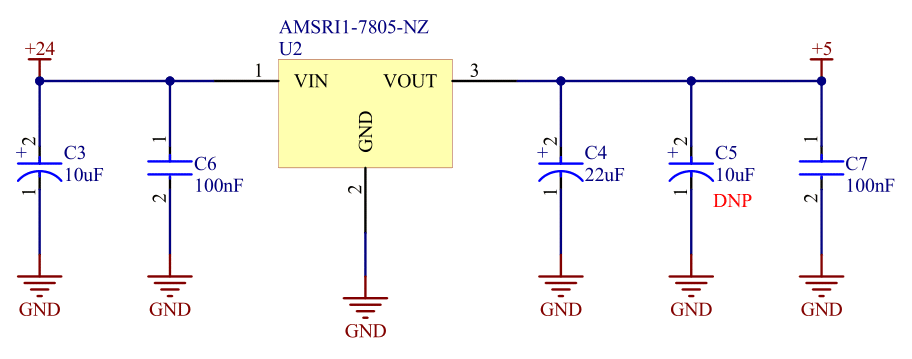
\includegraphics[width = 17cm]{images/zasilanie5v_3.png}
        \caption{Przetwornica przetwarzająca zasilanie 24V na 5V.} 
        \label{fig:sekcjaZasilania5v}
    \end{center}
\end{figure}

Następnie, napięcie 5V przetwarzane jest na 3.3V przy pomocy stabilizatora liniowego, widocznego na schemacie \ref{fig:sekcjaZasilania3v}.

\begin{figure}[h!]
    \begin{center}
        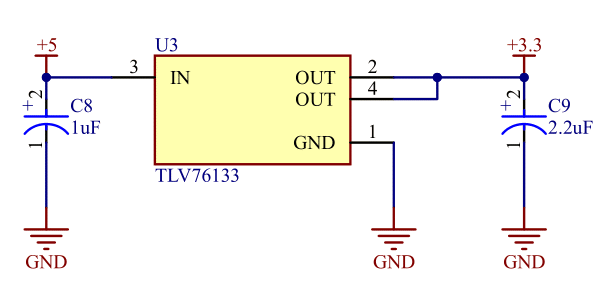
\includegraphics[width = 13cm]{images/zasilanie3v_3.png}
        \caption{Stabilizator liniowy 3.3V.} 
        \label{fig:sekcjaZasilania3v}
    \end{center}
\end{figure}

Pozwala to na ograniczenie szumów na linii 3.3V, która odpowiada za zasilanie układów takich jak mikrokontroler STM32, które mogą być wrażliwe na zmiany
napięcia zasilającego. Regulator TLV76133 \cite{TLV76133} jest kompatybilny wyprowadzeniowo z układami 1117. Jego maksymalny prąd wyjściowy to 1A i wymaga on jedynie niewielkich kondensatorów na swoim wejściu i wyjściu.

W celu zabezpieczenia znajdujących się na PCB elementów przed odwrotną polaryzacją oraz zwarciem, przy wejściu zasilającym zastosowano diody Schottkiego oraz bezpiecznik szeregowy.
Widoczne są one na rysunku \ref{fig:sekcjaZabezpieczn}.

\begin{figure}[h!]
    \begin{center}
        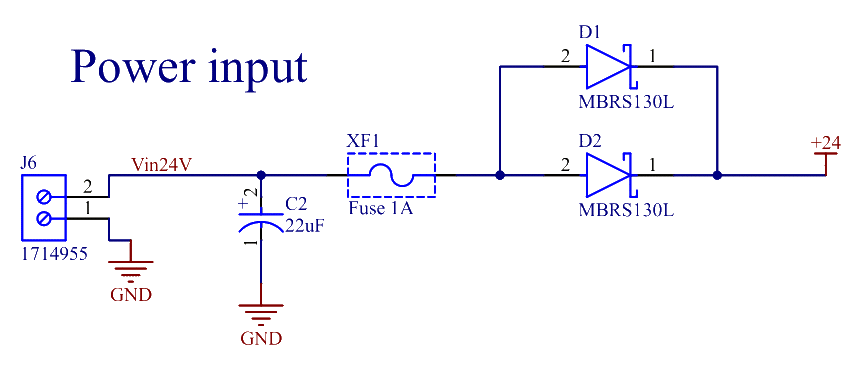
\includegraphics[width = 15cm]{images/wejsciezasilania_3.png}
        \caption{Zabezpieczenia wejścia zasilającego.} 
        \label{fig:sekcjaZabezpieczn}
    \end{center}
\end{figure}








\subsubsection{Pozostałe komponenty}

Moduł kontrolera posiada również wiele innych komponentów. Wśród nich są: 

\begin{itemize}
    \item buzzer - pozwalający na dźwiękowe powiadamianie, np. o zakończeniu procesu pomiaru,
    \item złącze USB typu B - z dodatkowym układem USBLC6 zabezpieczającym przed przepięciami,
    \item bateria RTC - pozwalająca na zapamiętanie stanu zegara i pracę układu RTC wbudowanego w mikrokontroler w tle, bez zewnętrznego zasilania,
    \item generatory kwarcowe - scalony generator o wyjściowym przebiegu 8Mhz zapewniający stabilną pracę interfejsów mikrokontrolera, takich jak USB oraz kwarc 32.768kHz przeznaczony dla układu wbudowanego zegara,
    \item sterownik wentylatorów - pozwalający na załączanie obciążeń zasilanych napięciem 24V, przeznaczony do sterowania znajdującymi się w obudowie urządzenia wentylatorami.
\end{itemize}

Układy te znaleźć można w załączniku na stronach „Moduł kontrolera: peryferia", „Moduł kontrolera: oscylatory" oraz „Moduł kontrolera: sterownik wentylatorów".

Schemat sterownika wentylatorów działa na zasadzie analogicznej, jak \ref{fig:sterowaniePodswietleniem}, umożliwiając załączanie wyższego napięcia (24V) poprzez wyjście GPIO mikrokontrolera.


\subsubsection{Projekt PCB}
\label{section:controllerPCB}

\begin{figure}[h!]
    \begin{center}
        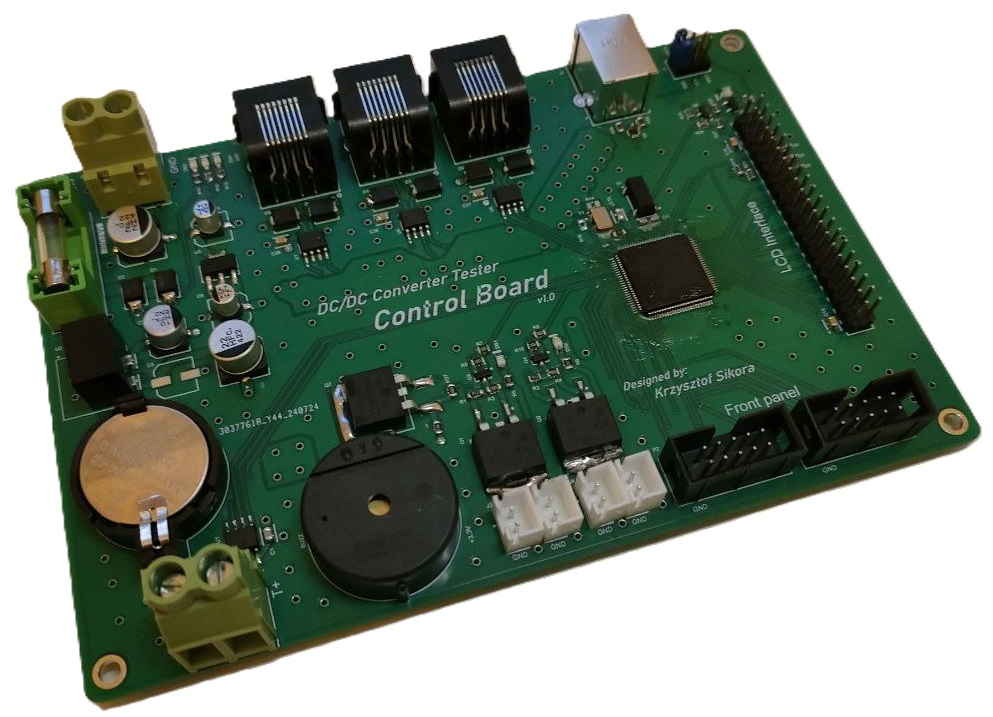
\includegraphics[width = 17cm]{images/controller_PCB.jpg}
        \caption{Zlutowana płytka PCB modułu kontrolera.} 
        \label{fig:modulkontroleraPCB}
    \end{center}
\end{figure}


Projekt PCB modułu kontrolera został wykonany z wykorzystaniem z oprogramowania Altium Designer.
Płytki wykonane zostały przez JLCPCB \cite{jlcpcb}. Płytka kontrolera ma wymiary 100 mm 
x 150 mm. Jest to PCB czterowarstwowe o grubości 1.6 mm. 

Wykorzystany został domyślny stackup producenta, przedstawiony na rysunku \ref{fig:stackupPCB}.
Górna oraz dolna warstwa miedzi wykorzystane zostały do prowadzenia sygnałów cyfrowych i analogowych. 
Warstwa druga (wewnętrzna) jest warstwą przeznaczoną dla linii zasilających (5 V, 3.3 V, 24 V), a trzecia 
jest warstwą masy (GND). Taki stackup pozwala na dokładną kontrolę impedancji, co wykorzystane zostało 
przy prowadzeniu ścieżek pary różnicowej sygnałów USB.

\begin{figure}[h!]
    \begin{center}
        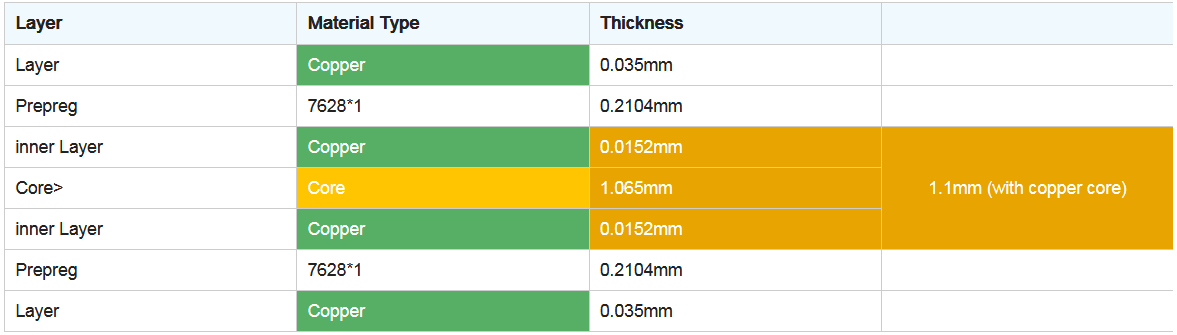
\includegraphics[width = 17cm]{images/stackupPCB.png}
        \caption{Wykorzystywany stackup PCB.} 
        \label{fig:stackupPCB}
    \end{center}
\end{figure}

Płytki PCB pozostałych modułów (zasilacza regulowanego oraz obciążenia aktywnego) wykonane zostały,
korzystając z tego samego stackupu. Posiadają one również takie same wymiary (szerokość i długość).


Na płytce kontrolera, przedstawionej na zdjęciu \ref{fig:modulkontroleraPCB}, widoczne są wszystkie omawiane 
w poprzednich punktach elementy. Z lewej strony zdjęcia widoczna jest sekcja zasilania, ze złączem wejściowym w 
górnej części. Poza przetwornicami 5 V i 3.3 V, widoczna jest również bateria zegara RTC - CR2032.
W dolnym lewym rogu umieszczono złącze termopary typu K, wraz z układem MAX6675. 
Do komunikacji wykorzystano złącza RJ45, umieszczone w górnej części PCB, wraz ze złączem USB typu B. 
Po stronie prawej widoczne jest 40-pinowe złącze wyświetlacza, a poniżej złącza IDC, służące do podłączenia 
paneli z przyciskami oraz złącza JST 2.5 mm, przeznaczone do zasilania wentylatorów.  

Centralny mikrokontroler STM32F4 jest otoczony przez układy oscylatorów HF oraz LF. Kondensatory filtrujące 
jego zasilanie, znajdują się na spodniej stronie płytki, co uprościło layout i pozwoliło zminimalizować 
pasożytnicze indukcyjności połączeń.

Widoczne tu ułożenie komponentów, w szczególności złącz, zostało ustalone w sposób, który umożliwił uproszczenie montażu mechanicznego
 w projektowanej obudowie, która przedstawiona została w sekcji \ref{section:mechanical}. 

Kompletny layout PCB, podzielony na poszczególne warstwy, przedstawiony został w załączniku.







\subsection{Zasilacz regulowany}
\label{section:zasilacz_regulowany}

Kolejnym modułem zaprojektowanym i zmontowanym w ramach projektu, jest moduł zasilacza regulowanego.
Został on zrealizowany w oparciu o przetwornicę impulsową obniżającą napięcie (buck). Pozwala ona na zasilanie 
układu testowanego (DUT). Napięcie wyjściowe ustalane jest przez wbudowany mikrokontroler, sterowany z modułu kontrolera.

\subsubsection{Przetwornica obniżająca napięcie}

Głównym elementem składowym modułu jest przetwornica napięciowa. Zdecydowano się skorzystać wyłącznie z przetwornicy impulsowej
bez dodatkowego regulatora liniowego, ze względu na prostszą konstrukcję i dużo wyższą sprawność, dzięki czemu nie ma konieczności wykorzystywania dodatkowego
radiatora. Ponadto, do celów testowania układów przetwornic, nie jest wymagana niska pojemność wyjściowa zasilacza, co jest 
często spotykane przy konstrukcjach zasilaczy laboratoryjnych. 

Wybrany układem scalonym przetwornicy obniżającej jest MP9928 \cite{MP9928}. Jest to układ przetwornicy synchronicznej,
pozwalający na zasilanie napięciem do 60V. Cechuje się stosunkowo wysoką maksymalną częstotliwością przełączania, równą 1 MHz i umożliwia sterowanie 
ze współczynnikiem wypełniania nawet 99.5\%. 

Z uwagi na to, że jest to przetwornica synchroniczna, do przełączania napięcia wejściowego wykorzystuje ona dwa zewnętrzne 
tranzystory, w tym przypadku typu N MOS. Oznacza to, że konieczne jest wykorzystanie układu bootstrap do przełączania jednego z tranzystorów.
Wybrane zostały polecane przez producenta tranzystory SQJ850EP \cite{SQJ850EP}. Poza świetnym $R_{DS}$ w stanie włączenia (nawet $0.023 \Omega$),
mają one także bardzo niski ładunek bramki (gate charge), na poziomie 20 nC, co umożliwia ich szybkie przełączanie i ogranicza straty.

Schemat przetwornicy został zaprezentowany na rysunku \ref{fig:MP9928schematic}.

\begin{sidewaysfigure}
    \begin{center}
        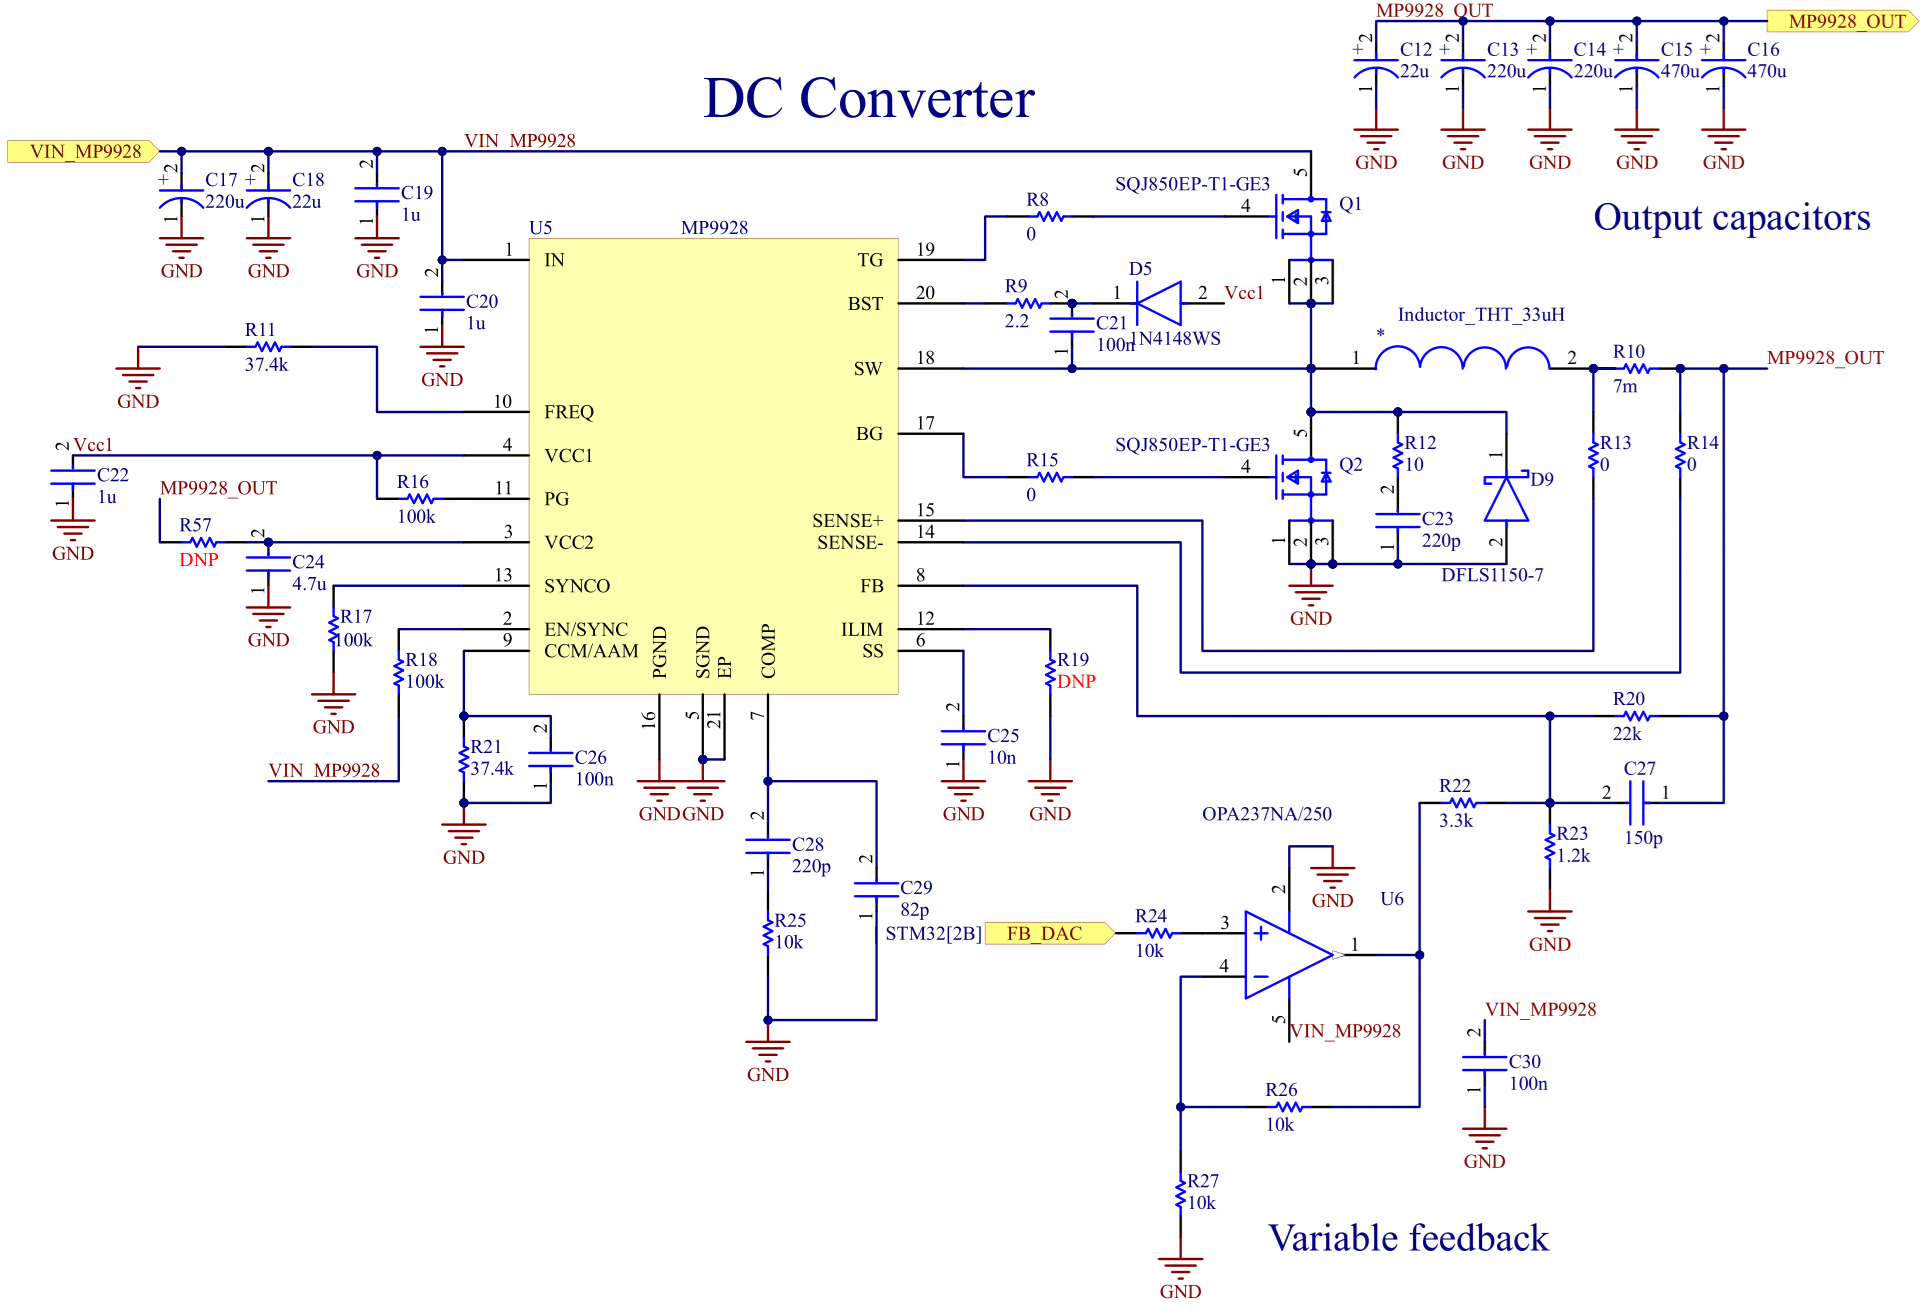
\includegraphics[width = 25cm]{images/przetwornicamp9928_3.png}
        \caption{Schemat układu przetwornicy MP9928.} 
        \label{fig:MP9928schematic}
    \end{center}
\end{sidewaysfigure}



Układ wzorowany był na płytce ewaluacyjnej od producenta Monolithic Power Systems Inc \cite{evalboardMP9928}.

W stosunku do niego, zmienione zostały jednak wartości wybranych kluczowych elementów. W celu ich doboru, skorzystano m.in.
z symulatora MPSmart \cite{mpsmart}. Jest to symulator oparty o narzędzia SIMetrix/SIMPLIS, przygotowany specjalnie 
w celach analizy działania układów przetwarzających moc. Pozwala on bowiem na symulację, wykorzystując metodę POP, czyli Periodic Operating Point,
co powala na szybszą analizę parametrów przetwornic, bez potrzeby korzystania z symulacji transient.

Początkowe wartości elementów takich jak: pojemność kondensatorów wejściowych, wyjściowych, czy też indukcyjność cewki przełączającej, obliczone zostały jednak ręcznie.
Niezbędne wzory zawarte są m.in. w książce Fundamentals of Power Electronics \cite{fundamentalsofpowerelectronics}.

W celu obliczenia wartości indukcyjności cewki, skorzystać można ze wzoru \ref{eq:4.1}.

\begin{equation}
    \label{eq:4.1}
    \begin{aligned}
        &L = \frac{V_{OUT} \cdot (V_{IN} - V_{OUT})}{V_{IN} \cdot \Delta I_{L} \cdot f_{s}} \\
        \\
        &\Delta I_{L} \approx 0.3 \cdot I_{LOAD}
    \end{aligned}
\end{equation}

$ \Delta I_{LOAD} $ jest to prąd tętnień cewki. Standardowo jego wartość przyjmuje się jako 30\% wartości prądu obciążenia, lecz może on być znacznie mniejszy.
Z równania \ref{eq:4.1}, po podstawieniu wartości napięć wejściowych, wyjściowych i prądu obciążenia otrzymujemy minimalną indukcyjność:

\begin{equation}
    \label{eq:4.2}
    L = \frac{20 V \cdot (24 V - 20 V)}{24 V \cdot  4 A \cdot 100 kHz} = 8.33 \mu H \\
\end{equation}

W celu obniżenia szumów, z uwagi na brak ograniczeń rozmiaru fizycznego, zdecydowano się na zwiększenie wartości indukcyjności do 22uH.
Dodatkowo, prąd saturacji cewki wynosić musi $I_{MAX}$, zgodnie z równaniem \ref{eq:4.3}.

\begin{equation}
    \label{eq:4.3}
    \begin{aligned}
        &I_{MAX} = I_{LOAD} + \frac{\Delta I_{L}}{2} \\ 
        \\ 
        &I_{MAX} = 3 A + \frac{1}{2} A = 3.5 A
    \end{aligned}
\end{equation}


Równie ważny jest wybór kondensatora/-ów na wyjściu przetwornicy. Aby zapewnić
niski poziom tętnień napięcia wyjściowego ($\Delta V_{out})$, muszą one mieć 
odpowiednio dużą pojemność. Można wyliczyć ją ze wzoru \ref{eq:4.4}.

\begin{equation}
    \label{eq:4.4}
    \begin{aligned}
        &C_{out} = \frac{\Delta I_{L}}{8 \cdot f_{s} \cdot \Delta V_{out}} \\ 
        \\ 
        &C_{out} = \frac{1 A}{8 \cdot 100kHz \cdot 1mV} \approx 1.25mF
    \end{aligned}
\end{equation}

Wartość ta ($1.25mF = 1250uF$) obliczona została dla tętnień napięcia wyjściowego
na poziomie 1mV, korzystając z noty \cite{obliczaniePojemnosciBuck}.


Po ustaleniu wartości podstawowych elementów przystąpiono do symulacji, która pozwoliła przetestować działanie przetwornicy i dokładnie dobrać wartości elementów wchodzących 
w skład obwodu kompensacji pętli sprzężenia zwrotnego.
Schemat wykorzystywany do symulacji przedstawiono poniżej \ref{fig:symulacjaMPSmart}.

\begin{figure}[h!]
    \begin{center}
        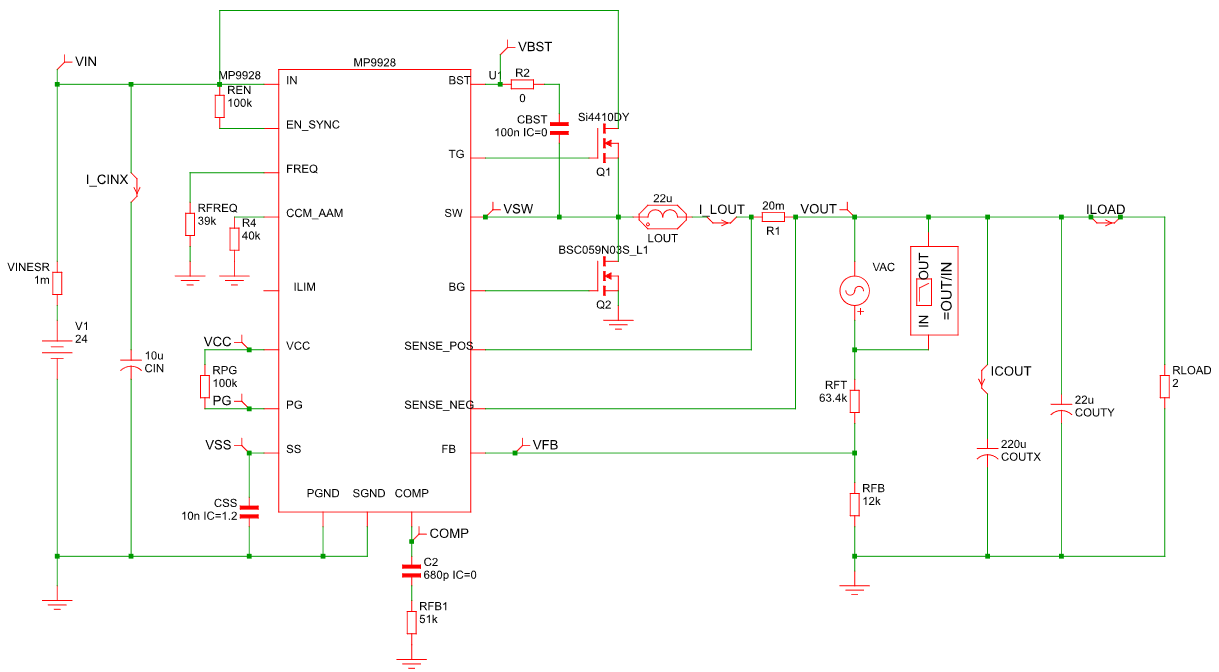
\includegraphics[width = 17cm]{images/schemat_do_symulacji_przetwornicy_MPSmart.png}
        \caption{Schemat wykorzystywany do symulacji w programie MPSmart.} 
        \label{fig:symulacjaMPSmart}
    \end{center}
\end{figure}

Jednym z wyników przeprowadzonych symulacji jest wykres bodego, 
przedstawiony na rysunku \ref{fig:napieciewyjsciowe1a5v}. Został on 
wygenerowany dla wyjściowego napięcia 5V 
przy prądzie 2A. Z przedstawionego wykresu można odczytać stabilność 
działania pętli sprzężenia zwrotnego przetwornicy, która w tym przypadku 
wynosi 82$\deg$. Jest to wartość fazy dla częstotliwości, dla której 
wzmocnienie (gain) wynosi 0dB. Wartość ta na wykresie jest dodatnia, z 
uwagi na stosowanie w przetwornicy napięciowej dodatniego sprzężenia zwrotnego.

\begin{figure}[h!]
    \begin{center}
        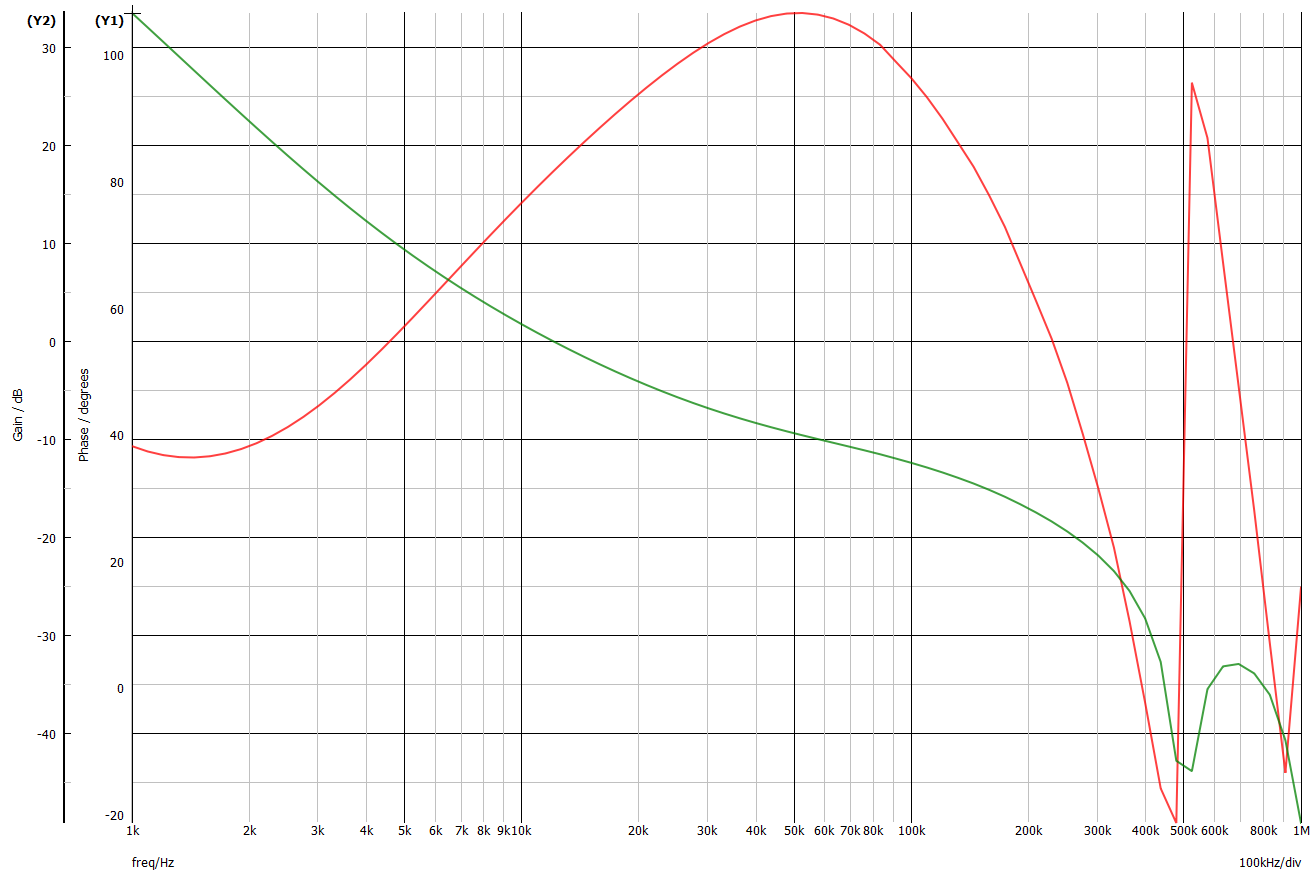
\includegraphics[width = 17cm]{images/bode_plot_przetwornica.png}
        \caption{Wykres bodego uzyskany z symulacji przetwornicy.} 
        \label{fig:napieciewyjsciowe1a5v}
    \end{center}
\end{figure}

Po przeprowadzeniu szeregu symulacji ustalone zostały wartości pozostałych elementów, które zawarte zostały na schemacie \ref{fig:MP9928schematic}. \\

Ważnym elementem, który pozwala na zmianę napięcia wyjściowego przetwornicy, jest układ, którego uproszczony schemat zawarty jest na rysunku \ref{fig:zmiananapieciaschemat}.

\begin{figure}[h!]
    \begin{center}
        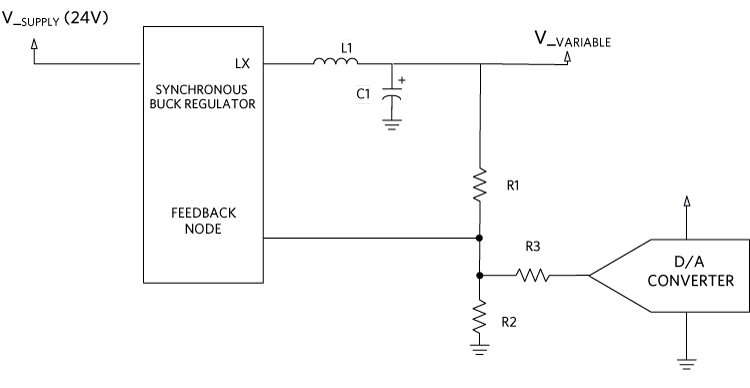
\includegraphics[width = 15cm]{images/variableoutput1_2.jpg}
        \caption{Schemat układu pozwalającego na zmianę napięcia wyjściowego przetwornicy. Źródło: \cite{variableoutput}.}
        \label{fig:zmiananapieciaschemat}
    \end{center}
\end{figure}

Dzięki niemu, zmieniając napięcie wyjściowe konwertera DAC (Digital to Analog Converter), w tym konkretnym przypadku wbudowanego w mikrokontroler STM32, można zmieniać napięcie wyjściowe przetwornicy impulsowej.

W celu łatwiejszego wyjaśnienia zasady działania tego układu, należy zauważyć, że układ scalony sterujący przetwornicą, dąży do
uzyskania na pinie FB (feedback) ustalonego napięcia, poprzez zmianę napięcia wyjściowego przetwornicy.
Układ ten, pod kątem funkcjonalnym, jest więc identyczny do układu przedstawionego na rysunku \ref{fig:variableoutput2}.

\begin{figure}[h!]
    \begin{center}
        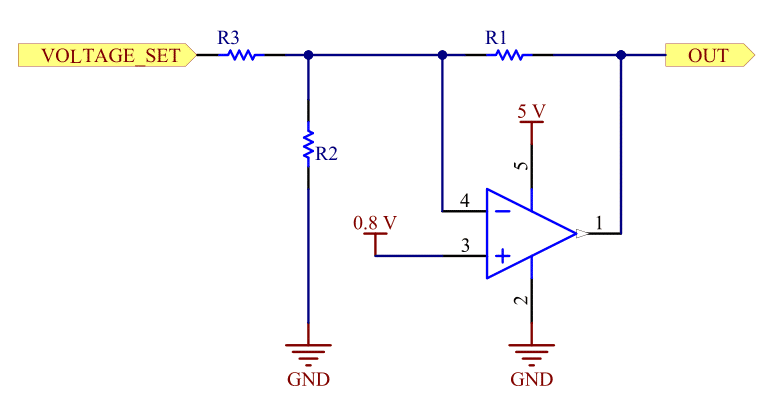
\includegraphics[width = 15cm]{images/voltageset55_3.png}
        \caption{Schemat pozwalający na analizę układu zmiany napięcia wyjściowego przetwornicy.}
        \label{fig:variableoutput2}
    \end{center}
\end{figure}

Analizując powyższy układ, można określić równanie \ref{eq:rownanienapieciawyjsciowego}.

\begin{equation}
    \label{eq:rownanienapieciawyjsciowego}
    \begin{aligned}
        V_{OUT} = V_{IN} \cdot (-\frac{R2}{R2+R3})(\frac{R1}{R2||R3}) + V_{REF} \cdot (1 + \frac{R1}{R2||R3})
    \end{aligned}
\end{equation}

Jak łatwo zauważyć, człon zawierający napięcie $V_{REF}$ wynika z zastosowania wzoru na wzmacniacz nieodwracający.
Z kolei współczynnik, przez który przemnażane jest napięcie $V_{IN}$ wynika bezpośrednio ze wzoru na wzmocnienie układu odwracającego.
Można zauwazyć, że napięcie wejściowe podzielone jest przez dzielnik napięcia, składający się z rezystorów R3 i R2.

Powyższe równanie przekształcić można w układ równań, pozwalający ustalić wartości rezystancji, przy założeniu danego zakresu napięcia z przetwornika
cyfrowo-analogowego oraz dla danego zakresu napięć wyjściowych.

\begin{equation}
    \label{eq:ukladrownanprzetwornica}
    \begin{aligned}
        \begin{cases}
            20 = m \cdot 0 + b \\
            0 = m \cdot 3 + b \\
        \end{cases} \\
        gdzie: \\
        \begin{cases}
            m = - (\frac{R2}{R2+R3})(\frac{R1}{R2||R3}) \\
            b = V_{REF} (1 + \frac{R1}{R2||R3})
        \end{cases}
    \end{aligned}
\end{equation}

Ustalone wartości rezystorów wynoszą odpowiednio:
\begin{equation}
    \label{eq:wartoscirezystorowprzetwornica}
    \begin{aligned}
        R1 = 22k \Omega \\
        R2 = 1.2k \Omega \\
        R3 = 3.3k \Omega \\
    \end{aligned}
\end{equation}




\subsubsection{Układ pomiaru prądu i napięcia}

W celu pomiaru mocy wyjściowej, czyli efektywnie mocy pobieranej przez podłączone urządzenie (DUT), zastosowany został specjalny układ umożliwiający 
pomiar napięcia wyjściowego i prądu wypływającego do obciążenia. Jego schemat przedstawiono poniżej na rysunku \ref{fig:pomiarpraduschemat}.

\begin{figure}[h!]
    \begin{center}
        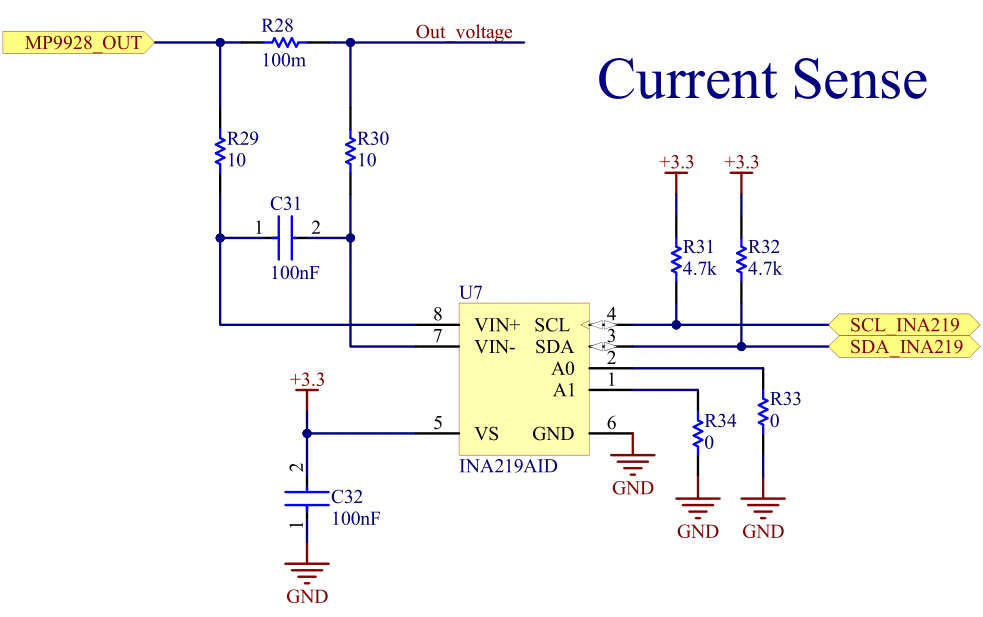
\includegraphics[width = 17cm]{images/pomiarpraduina219_3.png}
        \caption{Schemat układu służącego do pomiaru mocy wyjściowej.}
        \label{fig:pomiarpraduschemat}
    \end{center}
\end{figure}

W centrum schematu widoczny jest układ scalony INA219 \cite{ina219}. Umożliwia on pomiar napięć w zakresie 0 V do 26 V oraz pomiar prądu płynącego przez rezystor pomiarowy, na schemacie powyżej oznaczony 
jako R28.
W pełnym zakresie temperatur pracy producent deklaruje dokładność pomiaru na poziomie 0.5\% wartości mierzonej.
Pomiar dokonywany jest poprzez wbudowane przetworniki ADC (Analog to Digital Converter). Do pomiarów niewielkich napięć, układ wykorzystuje wbudowany 
PGA (Programmable Gain Amplifier), który umożliwia wzmocnienie sygnału wejściowego przed podaniem na wejście ADC. 
Następnie, wynik pomiaru zapisywany jest w odpowiednim rejestrze wewnętrznym układu, który odczytać można poprzez interfejs I2C.
Rezystory oznaczone jako R29 oraz R30, wraz z kondensatorem C31, służą do tłumienia szumów występujących na mierzonej linii zasilającej.
Elementy te są konieczne, jeśli w mierzonym sygnale wystąpić mogą szpilki napięciowe, bądź szumy o częstotliwościach powyżej 1 MHz, co należy uznać za prawdopodobne, jako że układ pomiarowy podłączony jest bezpośrednio do wyjścia 
modułu, podłączonego do innych urządzeń. \\


Zastosowanie układu INA219 gwarantuje uzyskanie dokładnego pomiaru prądu wyjściowego. Należy jednak zwrócić uwagę na powstały problem pomiaru napięcia wyjściowego, a dokładniej, napięcia na wejściu zasilanego urządzenia.
Poprzez zastosowanie rezystora pomiaru prądu, należy skompensować występujący na nim spadek napięcia. Dodatkowo, kolejny spadek napięcia wprowadzany jest przez przewody zasilające, 
zarówno te od dodatniej linii zasilania, jak i przewód masy. Napięcie dostarczone do obciążenia może być więc znacząco odmienne, od tego na wyjściu przetwornicy.

W celu kompensacji tego spadku zastosowany został dodatkowy układ pomiarowy, jak na schemacie \ref{fig:pomiarnapieciaroznicowo}.

\begin{figure}[h!]
    \begin{center}
        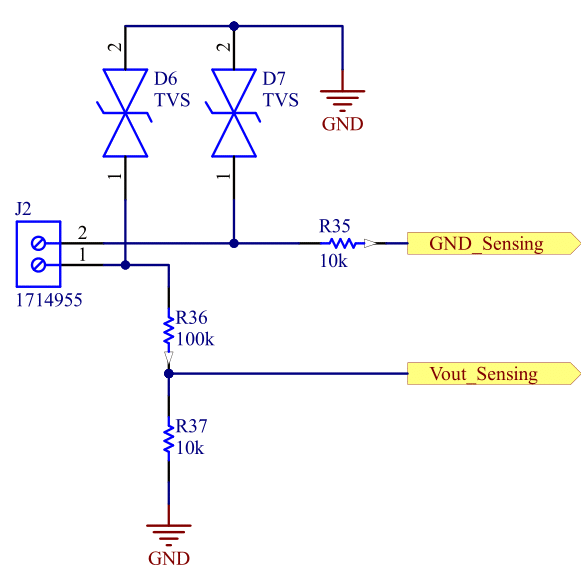
\includegraphics[width = 13cm]{images/pomiarnapieciaroznicowo_3.png}
        \caption{Schemat układu służącego do pomiaru napięcia dostarczanego do DUT.}
        \label{fig:pomiarnapieciaroznicowo}
    \end{center}
\end{figure}

Przedstawiony tu schemat składa się z jednego dzielnika napięciowego oraz zabezpieczeń w postaci diod TVS.
Przy pomocy dodatkowych wyprowadzeń, czyli złącza J2, oraz dodatkowych przewodów pomiarowych (sense leads), możliwy jest różnicowy pomiar napięcia.
Mierzone jest zarówno napięcie na dodatniej linii zasilającej, jak i na masie. Stosowanie dodatkowych przewodów, przez które płynie wyłącznie niewielki prąd pobierany przez przetworniki ADC,
zapobiega występowaniu spadków napięć na tychże przewodach, zwiększając dokładność pomiaru.

Do pomiaru wartości napięć $GND_Sensing$ oraz $Vout_Sensing$ wykorzystany został
przetwornik ADC wbudowany w mikrokontroler STM32. Umożliwia on pomiar napięć, 
które osiągają wartości bliskie ujemnemu napięciu zasilającemu przetwornik 
(w tym przypadku GND - 0 V), a dzięki zastosowaniu oddzielnego układu precyzyjnego 
napięcia referencyjnego, cechuje się wystarczającą precyzją, umożliwiając pomiar
z rozdzielczością 12 bitów.









\subsubsection{Mikrokontroler i dodatkowe układy}

Moduł zasilacza regulowanego sterowany jest poprzez mikrokontroler STM32F303K8T6 \cite{stm32f303}. 
Seria F3 od STMicroelectornics to układy przeznaczone do pracy w zastosowaniach mixed-signal, czyli 
łączących elementy cyfrowe z analogowymi. Wyposażone zostały one we wbudowane komparatory, wzmacniacze
operacyjne, precyzyjne przetworniki ADC oraz DAC, a także układy DSP (Digital Signal Processing) i 
FPU (Floating Point Unit). 

W projekcie modułu zasilacza wykorzystane zostały wbudowane układy ADC, służące do pomiaru napięcia na wejściu
testowanego układu (DUT) oraz układ DAC do ustalenia napięcia wyjściowego przetwornicy napięciowej.
Aby zapewnić wystarczającą dokładność pomiarów, wejście napięcia referencyjnego, które w przypadku
wybranego mikrokontrolera zasila również jego część analogową, podłączono do dedykowanego regulatora liniowego.
Wybranym układem jest LT1461CC \cite{lt1461}, a jego schemat przedstawiony został na rysunku \ref{fig:lt1461}.

\begin{figure}[h!]
    \begin{center}
        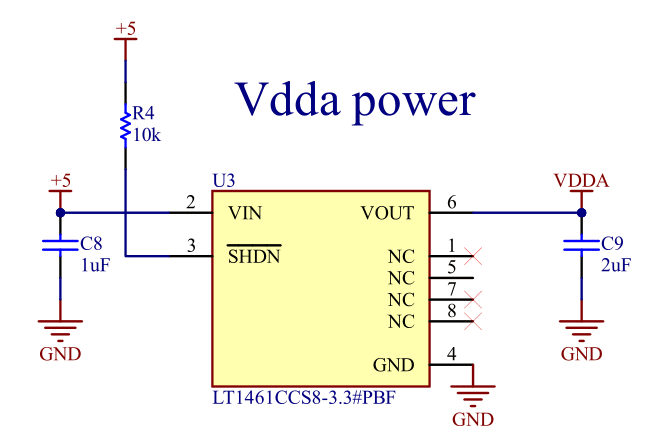
\includegraphics[width = 13cm]{images/lt1461_2.png}
        \caption{Schemat układu regulatora LT1461.}
        \label{fig:lt1461}
    \end{center}
\end{figure}

Jest to regulator liniowy, który w wersji L1461CS8-3.3 pozwala na uzyskanie na wyjściu stabilnego
napięcia 3.3 V, z maksymalnym prądem do 50mA. Napięcie wyjściowe ustalone jest z dokładnością do 
0.04\% i cechuje się niewielkim dryfem temperaturowym, do 3ppm/$^{\circ}$C.


Poza opisanymi wyżej komponentami, moduł zasilacza regulowanego posiada również kontroler
wentylatorów, sterowany przez mikrokontroler przekaźnik pozwalający na odłączenie wyjścia napięciowego modułu 
oraz czujnik temperatury LM75. Pomiar z czujnika temperatury może być zapisywany wraz
z innymi pomiarami, a także wykorzystywany jako wyzwalacz załączający wentylatory, zabezpieczając pozostałe układu.


\subsubsection{Projekt PCB}

\begin{figure}[h!]
    \begin{center}
        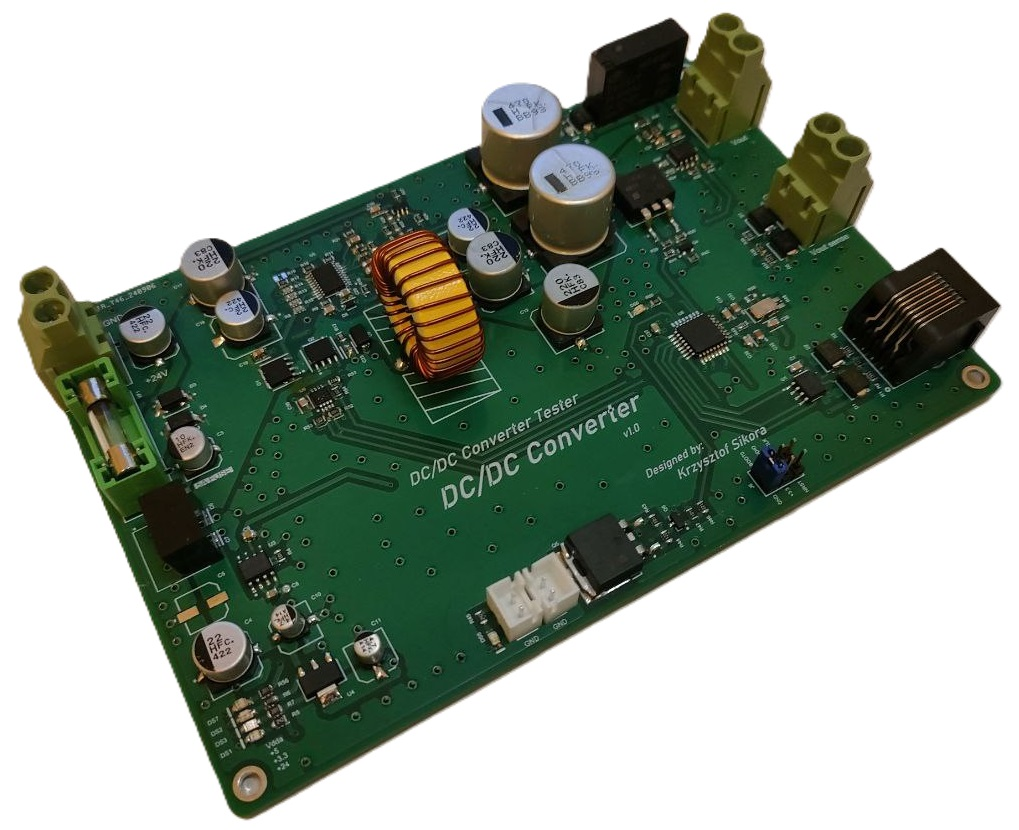
\includegraphics[width = 17cm]{images/converter_PCB.jpg}
        \caption{Zlutowana płytka PCB modułu zasilacza regulowanego.} 
        \label{fig:dcconverterPCB}
    \end{center}
\end{figure}

Przedstawione tu PCB (\ref{fig:dcconverterPCB}) jest to złożony moduł zasilacza regulowanego. Parametry płytki, 
takie jak stackup czy wymiary, są analogiczne do tych, które przedstawione zostały w sekcji \ref{section:controllerPCB}.

Z lewej strony zdjęcia widoczna jest sekcja zasilania, wraz ze złączem wejściowym. W części centralnej znajduje się 
przetwornica typu buck, oparta o układ MP9928, w obudowie TSSOP20-EP. Layout przetwornicy inspirowany był 
płytką deweloperską producenta \cite{evalboardMP9928}. Z uwagi na wykorzystanie cewki THT oraz większych kondensatorów 
wyjściowych jak i wejściowych, uległ on jednak znacznym modyfikacjom. Kluczowym aspektem było zachowanie jak 
najmniejszej impedancji połączeń elementów kluczujących, czyli tranzystorów NMOS, widocznych na płycie układu przetwornicy. 

W prawym górnym rogu PCB widoczne są kolejno złącza: wyjście napięciowe przetwornicy wraz z przekaźnikiem i układem 
pomiaru prądu, wejście napięcia SENSE, złącze RJ45 służące do komunikacji z kontrolerem.

Dokładny layout płytki przedstawiony został w załączniku.



\subsection{Obciążenie aktywne}

Trzecim zaprojektowanym i wykonanym modułem jest moduł obciążenia aktywnego. Jest to układ
bazujący na źródle prądowym, wykorzystującym pojedynczy tranzystor MOSFET. Umożliwia on obciążenie 
testowanego układu zadanym prądem. Prąd wyjściowy mierzonego układu ustalany jest poprzez mikrokontroler.
Analogicznie do przedstawionego wyżej modułu zasilacza regulowanego, sterowanie odbywa się poprzez interfejs RS485 
z modułu kontrolera.

\subsubsection{Układ ustalający prąd wyjściowy}

Najważniejszym elementem modułu obciążenia aktywnego jest sterowane źródło prądowe, przedstawione na schemacie \ref{fig:dcLoad}.

\begin{figure}[h!]
    \begin{center}
        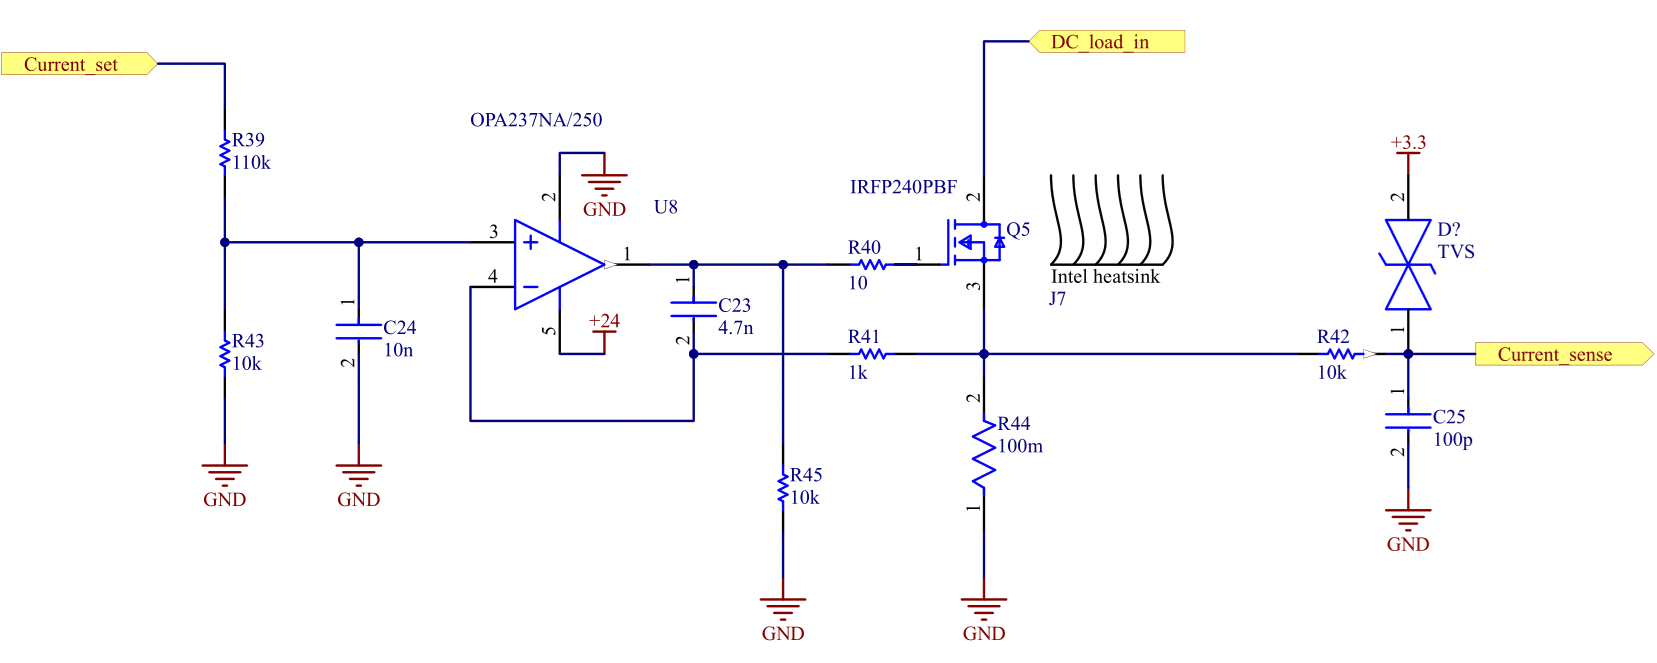
\includegraphics[width = 17cm]{images/dc_load_mosfet_2.png}
        \caption{Schemat układu sterowanego źródła prądowego.} 
        \label{fig:dcLoad}
    \end{center}
\end{figure}

Najważniejszym elementem układu jest MOSFET typu N, konkretnie model IRFP240PBF \cite{IRFP240} w obudowie TO-247AC.
Jego maksymalny ciągły prąd $I_{D}$ wynosi $12 A$, w temperaturze otoczenia $100^{\circ}$C, a maksymalne napięcie $U_{DS}$ wynosi 200 V.

Prąd wyjściowy jest ustalany poprzez napięcie na wyjściu $Current_set$. Poprzez dzielnik rezystancyjny podawane jest ono na wzmacniacz 
operacyjny OPA237. Do jego wejścia odwracającego podłączony jest rezystor R44, na którym mierzony jest prąd wyjściowy.
Wzmacniacz operacyjny ustala na swoim wyjściu napięcie, konieczne do wyrównania napięć na jego wyjściach, a więc 
steruje napięciem bramki MOSFETA Q5 ($V_{GS})$. Zmieniający się przez to prąd, powoduje zmianę napięcia na rezystorze pomiarowym R44.

Zgodnie z przedstawionym tu działaniem układu, zapisać można równanie \ref{eq:dc_load}.

\begin{equation}
    \label{eq:dc_load}
    \begin{aligned}
        I_{OUT} &= \frac{U_{R_{44}}}{R_{44}} \\
        gdzie: \\
        U_{R_{44}} &= U_{IN} \cdot \frac{10k \Omega}{10k \Omega + 110k \Omega}  \\
    \end{aligned}
\end{equation}

Ostatecznie, ustalony prąd wyjściowy jest więc dany wzorem \ref{eq:dc_load_current}.

\begin{equation}
    \label{eq:dc_load_current}
    \begin{aligned}
        I_{OUT} &= \frac{1}{12} \cdot \frac{U_{IN}}{100 m\Omega}
    \end{aligned}
\end{equation}

Zgodnie z założeniami projektu, napięcie wejściowe, które odkłada się na tranzystorze Q5 oraz rezystorze pomiarowym 
$R_{44}$, wynosi do 20 V, a maksymalny prąd to 2 A. W przedstawionym układzie możliwe jest jednak uzyskanie lepszych
parametrów. Zdecydowano się więc ustalić zakres prądu na 0 - 3 A. Maksymalna moc wydzielana wtedy w układzie wynosi jednak
$20 V \cdot 3 A = 60 W$. Oznacza to, że konieczne jest odpowiednie chłodzenie tranzystora MOSFET. 

Rozpatrzono dwa potencjalne rozwiązania problemu rozproszenia tak dużej mocy. Pierwszym jest zastosowanie wielu 
tranzystorów mocy połączonych równolegle. Pozwala ono na zastosowanie mniejszych tranzystorów (tj. o mniejszym prądzie drenu)
i podzielenie prądu między nie, zmniejszając wydzielaną na każdym z nich moc. To z kolei umożliwia montaż mniejszych radiatorów,
bądź montaż na wspólnym radiatorze, lecz z dużo większą całkowitą powierzchnią styku, a więc lepszym przewodnictwem cieplnym.
Rozwiązanie to nie jest jednak bez wad. Mimo, iż tranzystory MOS w znacznej większości przypadków posiadają ujemny współczynnik temperaturowy
prądu drenu, to dla niewielkich napięć $V_{GS}$, ten współczynnik może być dodatni. Opisuje to nota aplikacyjna AND8199/D \cite{parallelMOS}.
Mając na uwadze przedstawione tam wykresy, jak również potencjalną rozbieżność charakterystyk różnych tranzystorów,
należałoby zastosować oddzielne sterowanie bramek tranzystorów oraz niezależne rezystory pomiarowe na źródle każdego z nich.
Dzięki temu, zapewniony zostaje równy podział prądu, a więc również mocy, między poszczególne tranzystory. W przeciwnym wypadku, w przypadku 
uszkodzenia, czy też zmiany parametrów jednego z MOSFETów, może się okazać, że pozostałe z nich pracują z dużo większym prądem, doprowadzając do ich 
przegrzewania i kolejnych uszkodzeń.
Dla układów o niewielkich mocach, w tym takich jak przedstawiony, rozwiązanie to staje się bardziej kosztowne, z uwagi na 
dodatkową złożoność.
Zdecydowano się więc na drugą rozpatrywaną opcję, a więc zastosowanie pojedynczego tranzystora o większym prądzie drenu i 
maksymalnej rozpraszanej mocy. Zastosowany tranzystor cechuje się rezystancją termiczną junction-to-case 
na poziomie do 0.83 $^{\circ}$C/W.

Zgodnie z równaniem \ref{eq:thermalResistance}, wyliczyć można maksymalną rezystancję termiczną radiatora, dla 
podanej temperatury złącza (ang. \textit{junction}) tranzystora.

\begin{equation}
    \label{eq:thermalResistance}
    \begin{aligned}
        &T_{junction} = P \cdot (R_{thJC} + R_{heatsink}) + T_{ambient} \\
        &\text{gdzie:} \\
        &\text{$R_{heatsink}$ to rezystancja termiczna radiator-otoczenie} \\
        &\text{$T_{ambient}$ to temperatura otoczenia}
    \end{aligned}
\end{equation}

W równaniu tym pominięty jest wpływ rezystancji termicznej między tranzystorem a radiatorem. Wynika ona z
zastosowanego materiału termoprzewodzącego, takiego jak pasta termoprzewodząca, podkładka silikonowa.
Dla temperatury otoczenia $25^{\circ}C$ i maksymalnej temperatury $T_{junction} = 150^{\circ}C$, rezystancja radiatora wynosi \ref{eq:thermalResCalc}.

\begin{equation}
    \begin{aligned}
        150^{\circ}C &= 60 W \cdot (0.83 ^{\circ}C/W + R_{heatsink}) + 25^{\circ}C \\ 
        R_{heatsink} &\approx 1.25^{\circ}C/W
    \end{aligned}
    \label{eq:thermalResCalc}
\end{equation}

Przykładowy radiator przeznaczony do montażu na obudowie TO-247AC, przedstawiono na zdjęciu \ref{fig:typicalRadiator}.

\begin{figure}[h!]
    \begin{center}
        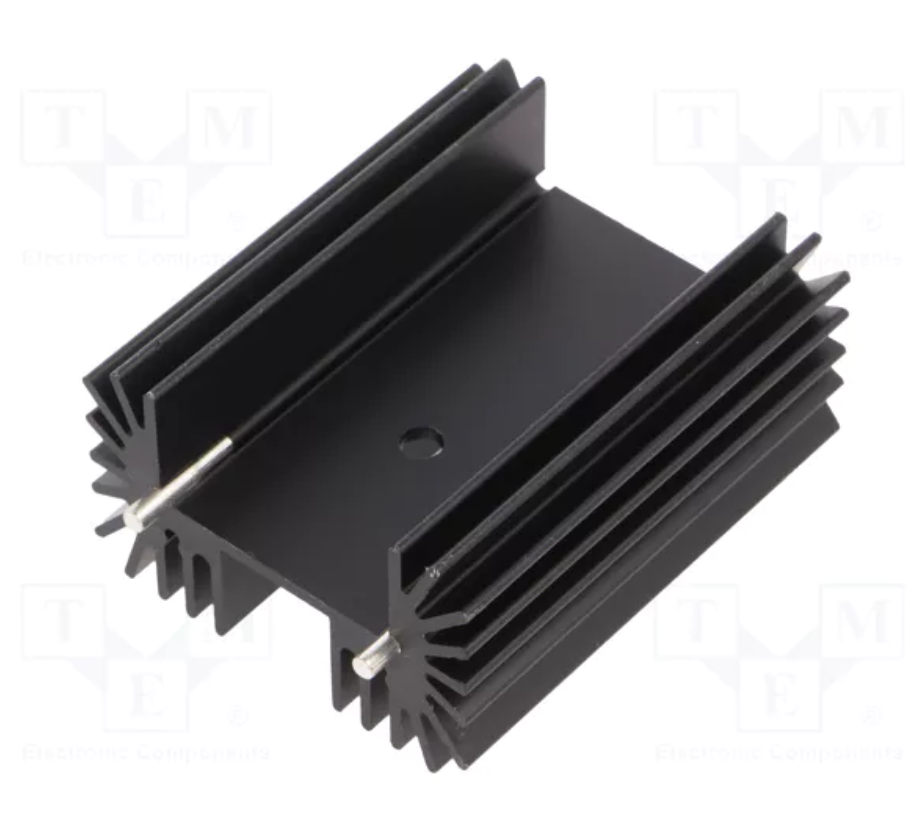
\includegraphics[width = 7cm]{images/typical_radiator.png}
        \caption{Przykładowy radiator do obudowy TO-247AC, model RA-T2X-51E \cite{RA-T2X-51E}.}
        \label{fig:typicalRadiator}
    \end{center}
\end{figure}

Jego rezystancja termiczna wynosi około 3.5$^{\circ}$C/W. 
Konieczne jest więc zastosowanie bardziej wydajnego radiatora, bądź też chłodzenia aktywnego. Radiatory takie są jednak dużo bardziej kosztowne. 
Tańszą alternatywą, którą zdecydowano się zastosować w projekcie, 
jest wykorzystanie chłodzenia przeznaczonego do innego typu układu, a konkretnie chłodzenia CPU \ref{fig:thermaltake} stosowanego w komputerach PC.

\begin{figure}[h!]
    \begin{center}
        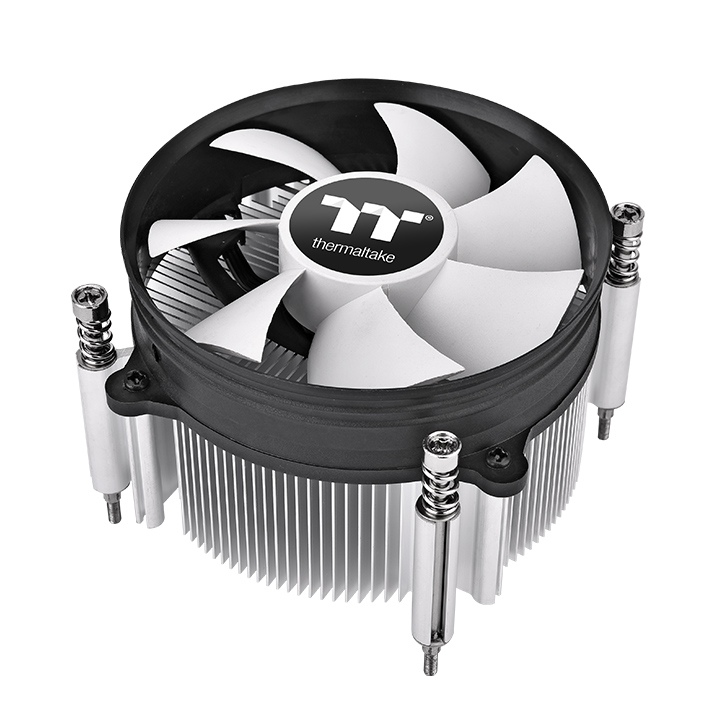
\includegraphics[width = 10cm]{images/gravityi3.jpg}
        \caption{Zastosowany radiator - Thermaltake Gravity i3.}
        \label{fig:thermaltake}
    \end{center}
\end{figure}

Zakupiony radiator, konkretnie Thermaltake Gravity i3 \cite{thermaltake}, nie posiada niestety w swojej specyfikacji konkretnego 
parametru rezystancji termicznej. Jest on przeznaczony do stosowania z procesorami na podstawkę LGA1700 o mocy do 95W, 
a więc z układami rozpraszającymi większą moc niż przewidywana. 






\subsubsection{Pozostałe układy}

Wśród pozostałych układów w module obciążenia aktywnego znalazły się:

\begin{itemize}
    \item mikrokontroler STM32F303K8T6,
    \item układ komunikacji RS485,
    \item układ pomiaru temperatury LM75,
    \item sterownik wentylatora 24V,
    \item układ pomiaru napięcia wejściowego SENSE,
    \item układ INA219 do pomiaru prądu i napięcia wejściowego.
\end{itemize}

Ich budowa jest analogiczna do przedstawionych w sekcji \ref{section:zasilacz_regulowany}.
Pozostałe schematy do modułu obciążenia aktywnego znajdują się również w załączniku.




\subsubsection{Projekt PCB}

\begin{figure}[h!]
    \begin{center}
        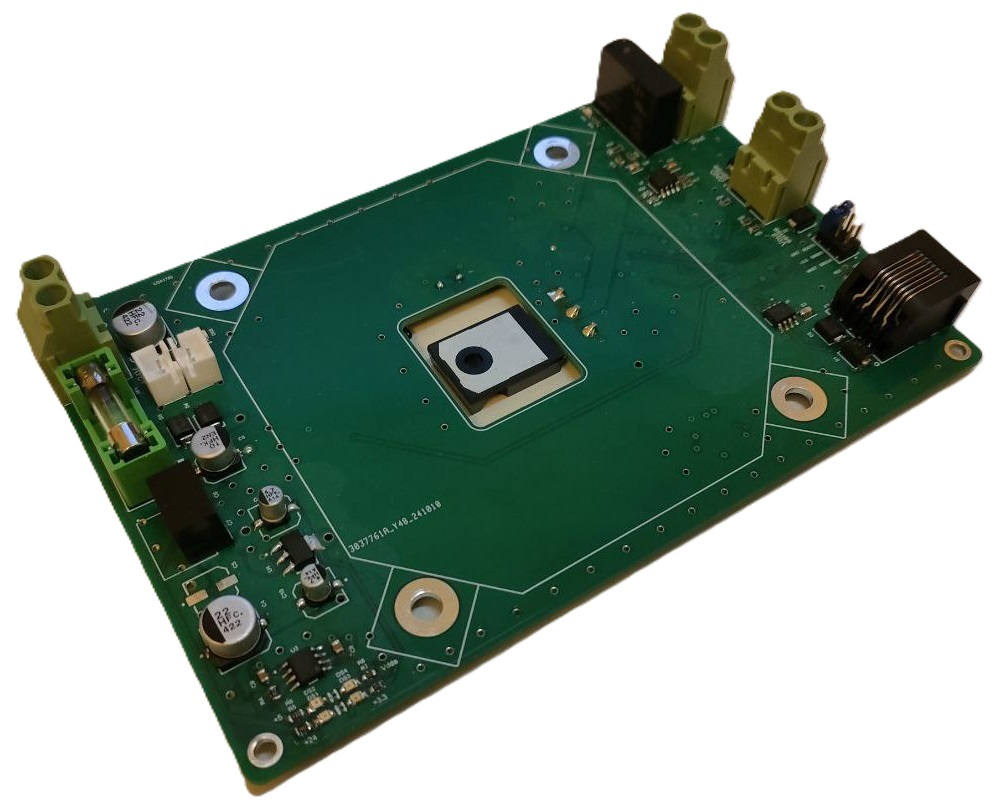
\includegraphics[width = 17cm]{images/dc_load_PCB.jpg}
        \caption{Zlutowana płytka PCB modułu obciążenia aktywnego.} 
        \label{fig:dcloadPCB}
    \end{center}
\end{figure}


Na rysunku \ref{fig:dcloadPCB} widoczne jest zlutowane PCB modułu obciążenia aktywnego. 
Złącza, znajdujące się na płytce, są ułożone w tych samych miejscach co w module zasilacza
regulowanego, który przedstawiony był już wcześniej (\ref{fig:dcconverterPCB}).

W samym centrum płytki widoczne jest prostokątne wycięcie, w którym umieszczony został MOSFET 
IRFP240. Na spodniej stronie płytki znalazł się także wzmacniacz operacyjny wraz z pozostałymi elementami,
które tworzą część analogową układu. Na dolnej stronie płytki umieszczony został również mikrokontroler.
Spowodowane to były umiejscowieniem radiatora, którego otwory montażowe i obrys widać na górnej stronie.
Z uwagi na jego rozmiar i ukształtowanie, konieczne było umiejscowienie elementów po przeciwnej stronie.

Tranzystor MOS musi być połączony z radiatorem w taki sposób, aby rezystancja termiczna tego połączenia 
była jak najmniejsza. Z uwagi na odległość kilku milimetrów, jaka powstaje między tylną powierzchnią
obudowy TO-247, a radiatorem, zastosowano podkładkę, wyciętą z płyty miedzianej. Połączenie między elementami
wypełnione jest poprzez elastyczne pady termiczne, a całość przykręcona do radiatora, w którym wcześniej
utworzono gwintowany otwór.

Dokładny layout płytki przedstawiony został w załączniku.



\FloatBarrier
\section{Oprogramowanie}

W ramach projektu napisano także oprogramowanie na mikrokontrolery STM32, które znajdują się 
w modułach kontrolera, zasilacza i obciążenia aktywnego. Firmware dla poszczególnych układów 
napisany został w języku C, korzystając przy tym z programu STM32CubeMX i udostępnionych przez producenta
bibliotek HAL (and. \textit{Hardware Abstraction Layer}).

W dalszej części podrozdziału opisano działanie powstałego oprogramowania, z podziałem na poszczególne moduły.

\subsection{Moduł kontrolera}
 
Moduł kontrolera zarządza działaniem podłączonych do niego układów, a jednocześnie pełni funkcję 
interfejsu użytkownika. Najważniejsze było więc zapewnienie intuicyjnej obsługi urządzenia, poprzez
stworzenie odpowiedniego menu. Zaimplementowano menu oparte o przedstawioną na rysunku \ref{fig:main_menu} hierarchię.

\begin{figure}[h!]
    \begin{center}
        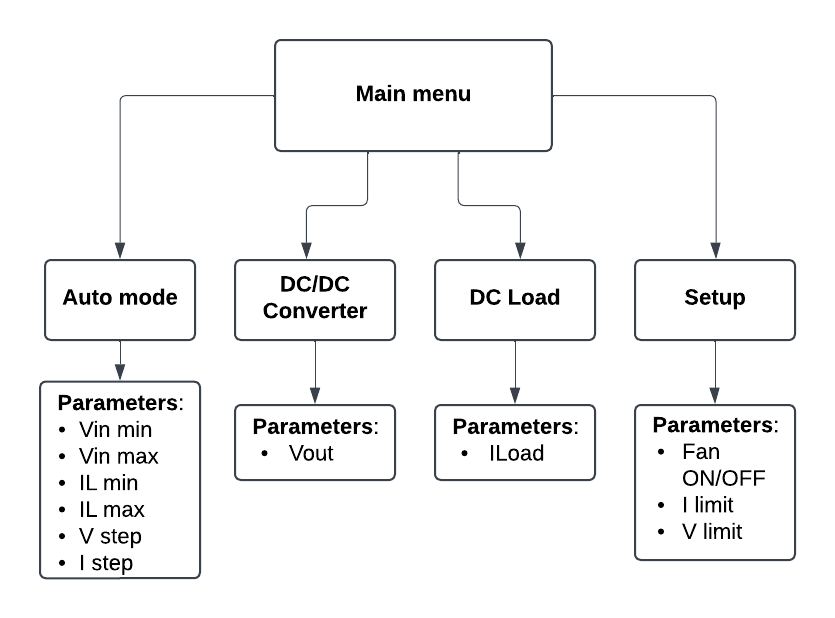
\includegraphics[width = 17cm]{images/menu_diagram.png}
        \caption{Schemat menu użytkownika zaimplementowany w projekcie.} 
        \label{fig:main_menu}
    \end{center}
\end{figure}

W oknie głównym (zdjęcie \ref{fig:main_menu_zdjecie}), przy pomocą przycisków (lewy, prawy), bądź enkodera,
użytkownik ma możliwość wyboru odpowiedniego podmenu. Przejść do niego można wciskając przycisk \textit{OK}.
Jednocześnie, wciskając przyciski \textit{DC\_ON}, \textit{LOAD\_ON}, możemy włączyć lub wyłączyć wyjście odpowiedniego modułu.

Odczyt stanu przycisków dokonywany jest w tym przypadku poprzez ciągły odczyt stanu danego wejścia. 
W tym czasie, mikrokontroler nie musi bowiem wykonywać żadnej dodatkowej czynności. Odczyt stanu enkodera 
(obrót) dokonywany jest, korzystając z trybu \textit{encoder mode} licznika wbudowanego w STM32.
Dzięki temu możliwe jest sprawdzenie, czy enkoder został obrócony i o ile, odczytując wartość pojedynczego rejestru.

\begin{figure}[h!]
    \begin{center}
        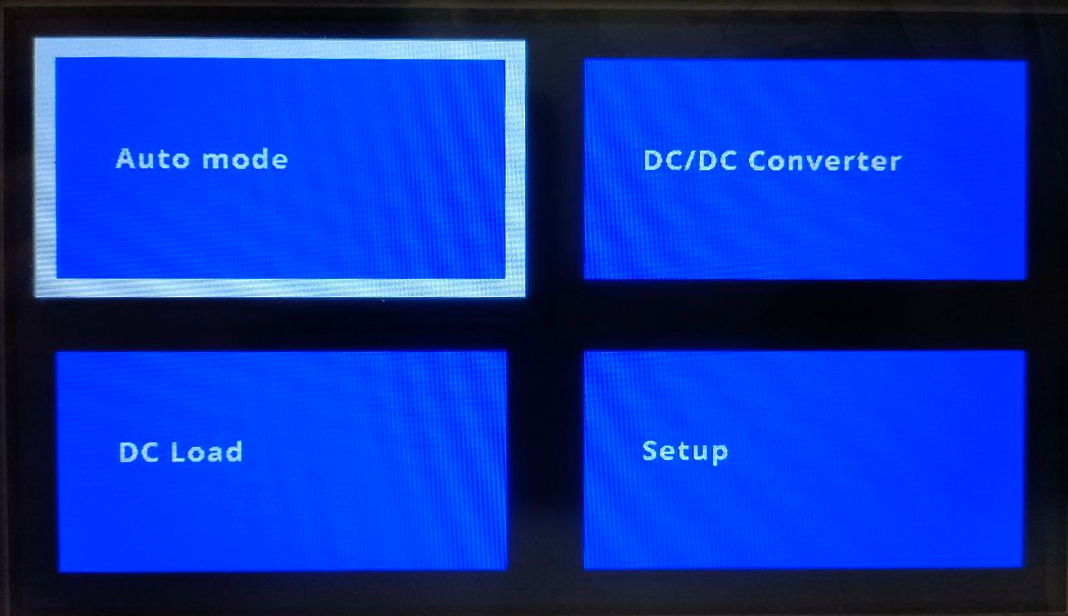
\includegraphics[width = 13cm]{images/main_menu_zdjece.jpg}
        \caption{Zdjęcie menu głównego urządzenia.} 
        \label{fig:main_menu_zdjecie}
    \end{center}
\end{figure}

Wciśnięcie jednego z przycisków, odpowiadających za przełączenie wyjścia innego modułu, powoduje wysłanie ramki z odpowiednią komendą do wybranego modułu.
Możliwe do wysłania komendy zawarto w przedstawionym typie enumeracyjnym \ref{lst:enum}.

\begin{lstlisting}[label=lst:enum,caption=Lista dostępnych komend przesyłanych poprzez RS485., float,frame=tb]
typedef enum
{
    CMD_SET_OUTPUT_VOLTAGE = 0x01,
    CMD_TURN_OUTPUT_ON = 0x02,
    CMD_TURN_OUTPUT_OFF = 0x03,
    CMD_TURN_FAN_ON = 0x04,
    CMD_TURN_FAN_OFF = 0x05,
    CMD_READ_TEMPERATURE = 0x06,
    CMD_READ_CURRENT = 0x07,
    CMD_READ_OUTPUT_VOLTAGE = 0x08,
    CMD_SET_CURRENT = 0x09,
    CMD_ACKNOWLEDGE = 0x10,
    CMD_READ_SENSE_VOLTAGE = 0x11,
    CMD_READ_CURRENT_SENSE = 0x12
} CommandType;
\end{lstlisting}

Do obsługi wyświetlacza, opartego o kontroler SSD1963, wykorzystano gotowy driver \cite{SSD1963_DRIVER}, który zmodyfikowano, aby przyspieszyć jego 
działanie poprzez bezpośrednią modyfikację rejestrów, z pominięciem HAL.

Komendy wysyłane są do pozostałych modułów za pośrednictwem interfejsu UART, korzystając z funkcji
wbudowanych w biblioteki HAL. Aby zapewnić możliwość dalszej rozbudowy projektu o inne urządzenia, 
każdy moduł definiowany jest w postaci struktury, której przykład przedstawia kod \ref{lst:dcstruct}.

Zdefiniowany jest tutaj numer fizycznego portu UART, adres urządzenia na magistrali i nazwa.
Struktura przechowuje również wskaźniki na uniwersalne funkcje do wysyłania i odbierania danych.

\begin{lstlisting}[label=lst:dcstruct,caption=Przykładowa struktura definiująca moduł., float,frame=tb]
DeviceModule dc_dc_converter =
{
    .name = "DC/DC Converter",
    .uart_number = 2,
    .device_address = 1,
    .sendCommand = UART_SendCommand,
    .receiveCommand = UART_ReceiveCommand,
};
\end{lstlisting}

Dzięki temu, możliwe jest wykorzystanie tych samych funkcji do obsługi wielu modułów. Przykładowo, kod \ref{lst:exampleFanON},
przedstawia funkcję załączającą wentylator w module.

\begin{lstlisting}[label=lst:exampleFanON,caption=Przykładowa funkcja załączająca wentylator w module, float,frame=tb]
uint8_t Fan_On(DeviceModule* module)
{
    CommandPacket cmd;
    cmd.command = CMD_TURN_FAN_ON;

    // Send the command
    module->sendCommand(module->uart_number, &cmd);

    return module->receiveCommand(module->uart_number, &cmd);
}
\end{lstlisting}

Wywołując funkcję, podaje się wskaźnik na strukturę odpowiedniego modułu, która zawiera wszystkie informacje konieczne do
przesłania komendy do konkretnego modułu.

Menu \textit{Auto mode} oraz \textit{DC/DC Converter} zostały przedstawione na kolejnych zdjęciach \ref{fig:zdjecia_menu_auto}.
Menu \textit{DC Load} zostało zaprogramowane analogicznie do \textit{DC/DC Converter}.


\begin{figure}[h!]%
    \centering
    \subfloat[\centering]{{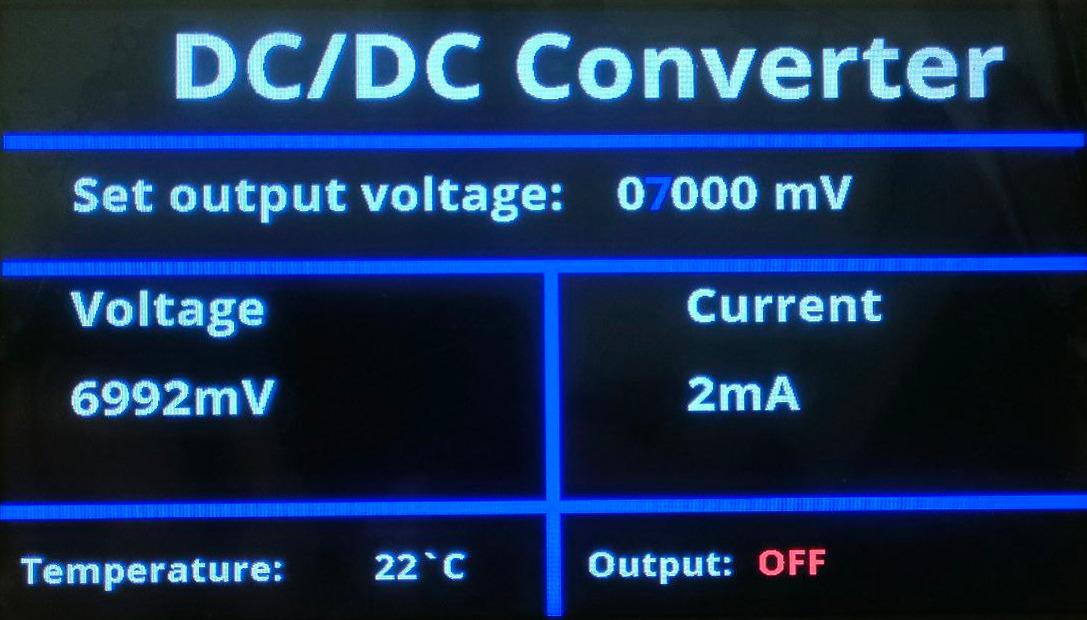
\includegraphics[width=7cm]{images/dc_converter_menu_zdjecie.jpg} }}%
    \qquad
    \subfloat[\centering]{{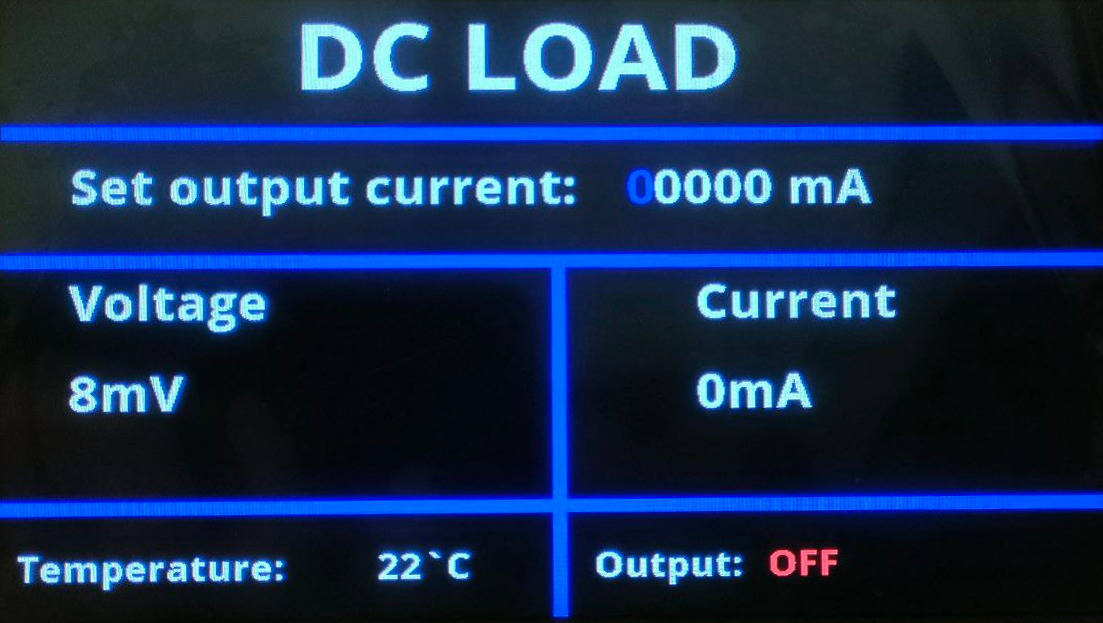
\includegraphics[width=7cm]{images/dc_load_menu_zdjecie.jpg} }}%
    \caption{Wygląd pozostałych menu.}
    \label{fig:zdjecia_menu_auto}%
\end{figure}

Pozwalają one na zmianę przedstawionych wcześniej na rysunku \ref{fig:main_menu} parametrów. Można tego dokonać za pomocą 
zarówno przycisków, jak i enkodera, zmieniając niezależnie kolejne cyfry ustawianego napięcia, bądź prądu, zapisane w miliwoltach.

Po ustawieniu odpowiednich parametrów menu zasilacza regulowanego oraz obciążenia aktywnego zaczynają wyświetlać 
mierzony prąd wyjściowy i napięcia. 

Po konfiguracji \textit{Auto menu} następuje natomiast automatyczny pomiar sprawności podłączonej do urządzenia przetwornicy.
Efektem tego pomiaru jest wykres sprawności. Przykładowy wykres przedstawiony został w rozdziale \ref{chapter-5}.



%\subsection{Moduł zasilacza regulowanego}
\FloatBarrier
\subsection{Pozostałe moduły}

Pozostałe moduły, stanowiące urządzenia podrzędne, oczekują na komendę otrzymaną od kontrolera. W związku z tym, 
w głównej pętli programu, kontrolują one jedynie wartości mierzonych parametrów. Są wśród nich m.in. napięcie wyjściowe, 
prąd wyjściowy, temperatura modułu, stan wejść pomiarowych. W wypadku przekroczenia bezpiecznego limitu któregokolwiek z 
parametrów, wyłączone zostaje wyjście modułu (przekaźnik), a napięcie lub prąd wyjściowy ustawiony jest na wartość 0 V / 0 A.

Komendy odbierane poprzez interfejs UART, rozpoczynają procedurę przerwania. Następnie, odebrana ramka jest analizowana
i w zależności od odebranej komendy podejmowana jest odpowiednia akcja, a następnie odsyłana odpowiedź. W przypadku 
odbioru komendy, która nie jest obsługiwana przez moduł, nie jest odsyłana odpowiedź (ACK - ang. \textit{Acknowledge}).

Diagram przedstawiający opisane działanie przedstawiono na rysunku \ref{fig:submodule_code_diagram}.

\begin{figure}[h!]
    \begin{center}
        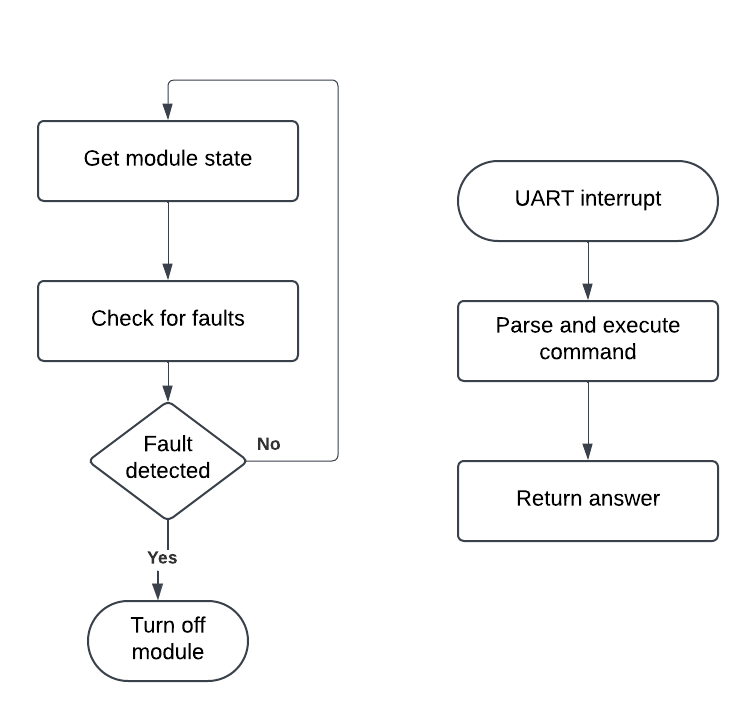
\includegraphics[width = 11cm]{images/submodule_code_diagram.png}
        \caption{Diagram przedstawiający działanie kodu modułu.} 
        \label{fig:submodule_code_diagram}
    \end{center}
\end{figure}

Skrócony kod przerwania przedstawiono we fragmencie \ref{lst:interruptCode}.

\begin{lstlisting}[label=lst:interruptCode,caption=Funkcja odpowiadająca za ustawienie napięcia wyjściowego., float,frame=tb]
void HAL_UART_RxCpltCallback(UART_HandleTypeDef *huart)
{
  CommandPacket receivedPacket, CommandPacket returnPacket;
  unsigned char return_message[3] = "";

  receivedPacket.command = rx_buff[0];
  receivedPacket.data[0] = rx_buff[1];
  receivedPacket.data[1] = rx_buff[2];

  switch(receivedPacket.command)
  {
    case CMD_SET_OUTPUT_VOLTAGE:
      float setVoltage = ((receivedPacket.data[0] << 8) | receivedPacket.data[1]) / 100.0; // 500 (0x01F4) means 5V etc
      Set_Output_Voltage(setVoltage);
      returnPacket.command = CMD_ACKNOWLEDGE;
      returnPacket.data[0] = receivedPacket.data[0];
      returnPacket.data[1] = receivedPacket.data[1];
      break;

    ...
  }

  return_message[0] = returnPacket.command;
  return_message[1] = returnPacket.data[0];
  return_message[2] = returnPacket.data[1];

  HAL_GPIO_WritePin(Dir1_GPIO_Port, Dir1_Pin, GPIO_PIN_SET);
  HAL_UART_Transmit(&huart1, return_message, sizeof(return_message), 100);
  HAL_GPIO_WritePin(Dir1_GPIO_Port, Dir1_Pin, GPIO_PIN_RESET);

  memset(rx_buff, 0, sizeof(rx_buff));
  HAL_UART_Receive_IT(&huart1, rx_buff, 3);
}
\end{lstlisting}

Najważniejszym zadaniem modułu zasilacza regulowanego jest zmiana napięcia wyjściowego. Odpowiedzialna za to funkcja 
przedstawiona została we fragmencie kodu \ref{lst:dcVoltageSet}.
Implementuje ona wzór, który jest przekształceniem równania \ref{eq:rownanienapieciawyjsciowego}.

\begin{lstlisting}[label=lst:dcVoltageSet,caption=Funkcja odpowiadająca za ustawienie napięcia wyjściowego., float,frame=tb]
void Set_Output_Voltage(float voltage)
{
	float DAC_Voltage = 1.56 - 0.075 * voltage;

	uint32_t var = (uint32_t)(DAC_Voltage*ADC_BITS)/ADC_REFERENCE_VOLTAGE;

	HAL_DAC_SetValue(&hdac1, DAC1_CHANNEL_1, DAC_ALIGN_12B_R, var);
}
\end{lstlisting}

Analogicznie, we fragmencie \ref{lst:currentSetCode}, przedstawiono funkcję ustawiającą prąd wyjściowy modułu obciążenia aktywnego, 
implementującą wzór \ref{eq:dc_load_current}.

\begin{lstlisting}[label=lst:currentSetCode,caption=Funkcja odpowiadająca za ustawienie prądu wyjściowego., float,frame=tb]
void Set_Output_Current(float current)
{
	float DAC_Voltage = current * 1.3;

	uint32_t var = (uint32_t)(DAC_Voltage*ADC_BITS)/ADC_REFERENCE_VOLTAGE;

	HAL_DAC_SetValue(&hdac1, DAC1_CHANNEL_1, DAC_ALIGN_12B_R, var);
}
\end{lstlisting}

Obie te funkcje wykorzystują wbudowane przetworniki DAC, korzystając z funkcji \textit{HAL\_DAC\_SetValue()}.
Do odczytu rejestrów układów INA219 (do pomiaru prądu i napięcia) oraz LM75 (do pomiaru temperatury), wykorzystywane są funkcje
\textit{HAL\_I2C\_Mem\_Read()}. Przykładowo, kod \ref{lst:pomiarTemperaturyCode} zawiera funkcje odczytującą temperaturę układu.

\begin{lstlisting}[label=lst:pomiarTemperaturyCode,caption=Funkcja odczytująca temperaturę z układu LM75., float,frame=tb]
float LM75_Read_Temperature()
{
    unsigned char buffer[2];

    HAL_I2C_Mem_Read(&hi2c1, (LM75_ADDR), LM75_Temp, 1, buffer, 2, 1000);

    float output = ((buffer[0] << 8) | buffer[1]) / 256.0;

    return output;
}
\end{lstlisting}

%\subsection{Moduł obciążenia aktywnego}




\FloatBarrier
\section{Mechanika}
\label{section:mechanical}


Poza częścią elektroniczną wraz z oprogramowaniem, stworzono również kompletny projekt obudowy, korzystając z 
programu Fusion 360, na licencji studenckiej \cite{fusion360}. 

Projekt części mechanicznej powstawał równolegle do projektu elektroniki, dzięki czemu możliwe było dopasowanie
rozkładu złącz płytek PCB oraz wytworzenie odpowiedniego okablowania. Render przedstawiający widok zewnętrzny 
widoczny jest na rysunku \ref{fig:mechanical_Render}.

\begin{figure}[h!]
    \begin{center}
        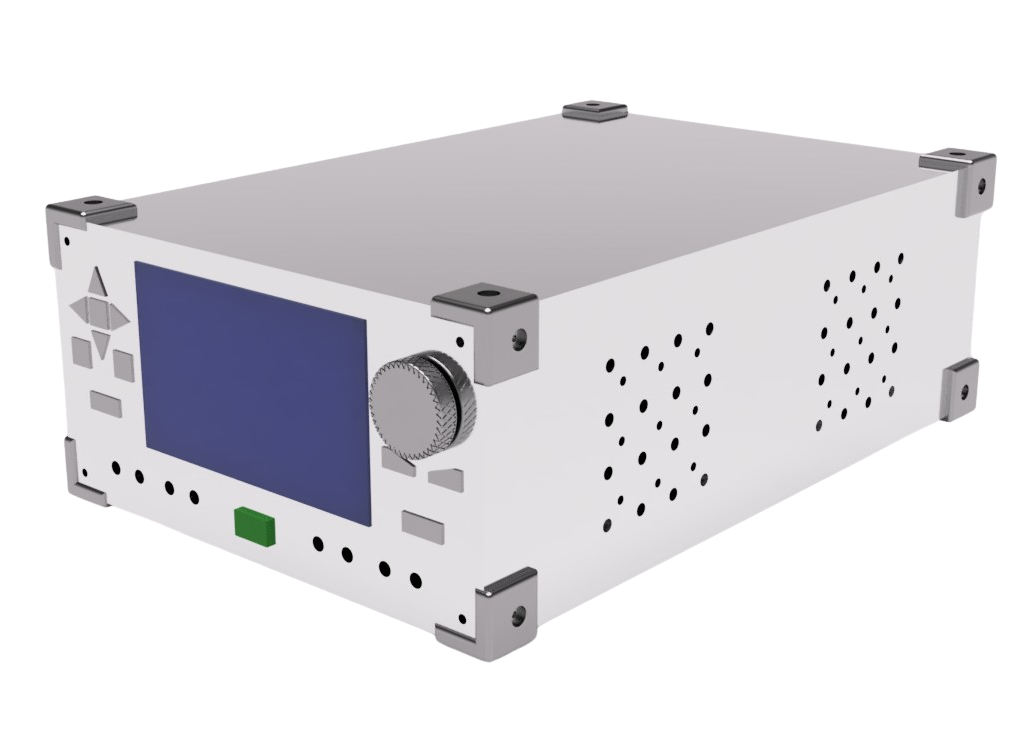
\includegraphics[width = 17cm]{images/obudowa_render-removebg.png}
        \caption{Render obudowy projektu wykonany w programie Fusion 360.} 
        \label{fig:mechanical_Render}
    \end{center}
\end{figure}

Projekt oparty został o stelaż z profili aluminiowych 2020 (20 mm x 20 mm), które umożliwiają montaż pozostałych elementów
dzięki nakrętkom młoteczkowym. Panele zewnętrzne wykonane zostały z aluminium o grubości 3 mm. Wycięte już na odpowiedni wymiar 
panele należało poddać obróbce w celu wykonania otworów na złącza, przyciski oraz wyświetlacz. Wykonano je na frezarce 
3-osiowej - zmodyfikowanym urządzeniu Vevor 3018. Do stworzenia g-code wykorzystano narzędzie wbudowane w oprogramowanie 
Fusion 360, a następnie zmodyfikowano ręcznie w programie UGS (Universal G-code Sender) \ref{fig:ugs}.

\begin{figure}[h!]%
    \centering
    \subfloat[\centering Wizualizator UGS.]{{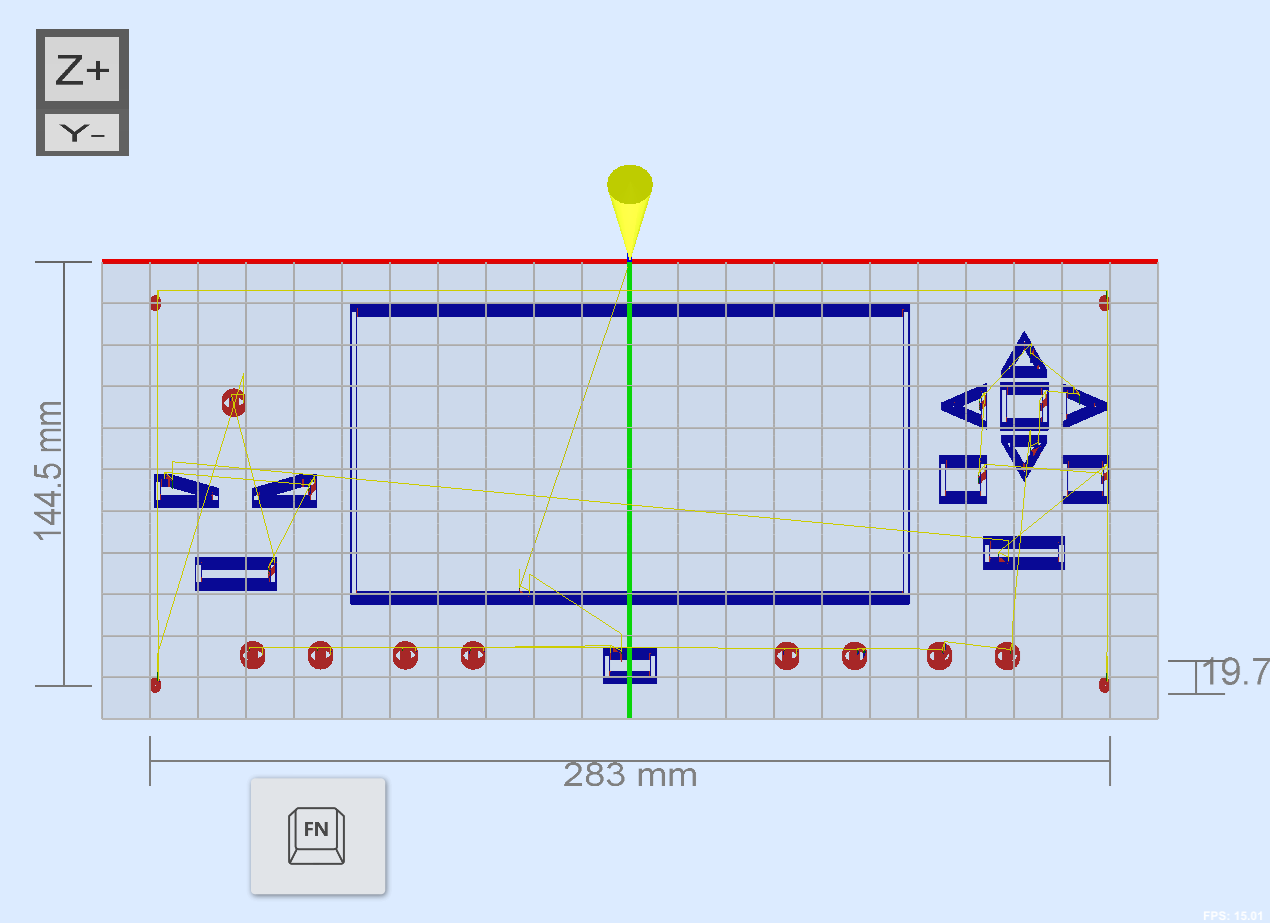
\includegraphics[width=7.5cm]{images/ugs.png} }}%
    \qquad
    \subfloat[\centering Frezarka 3018.]{{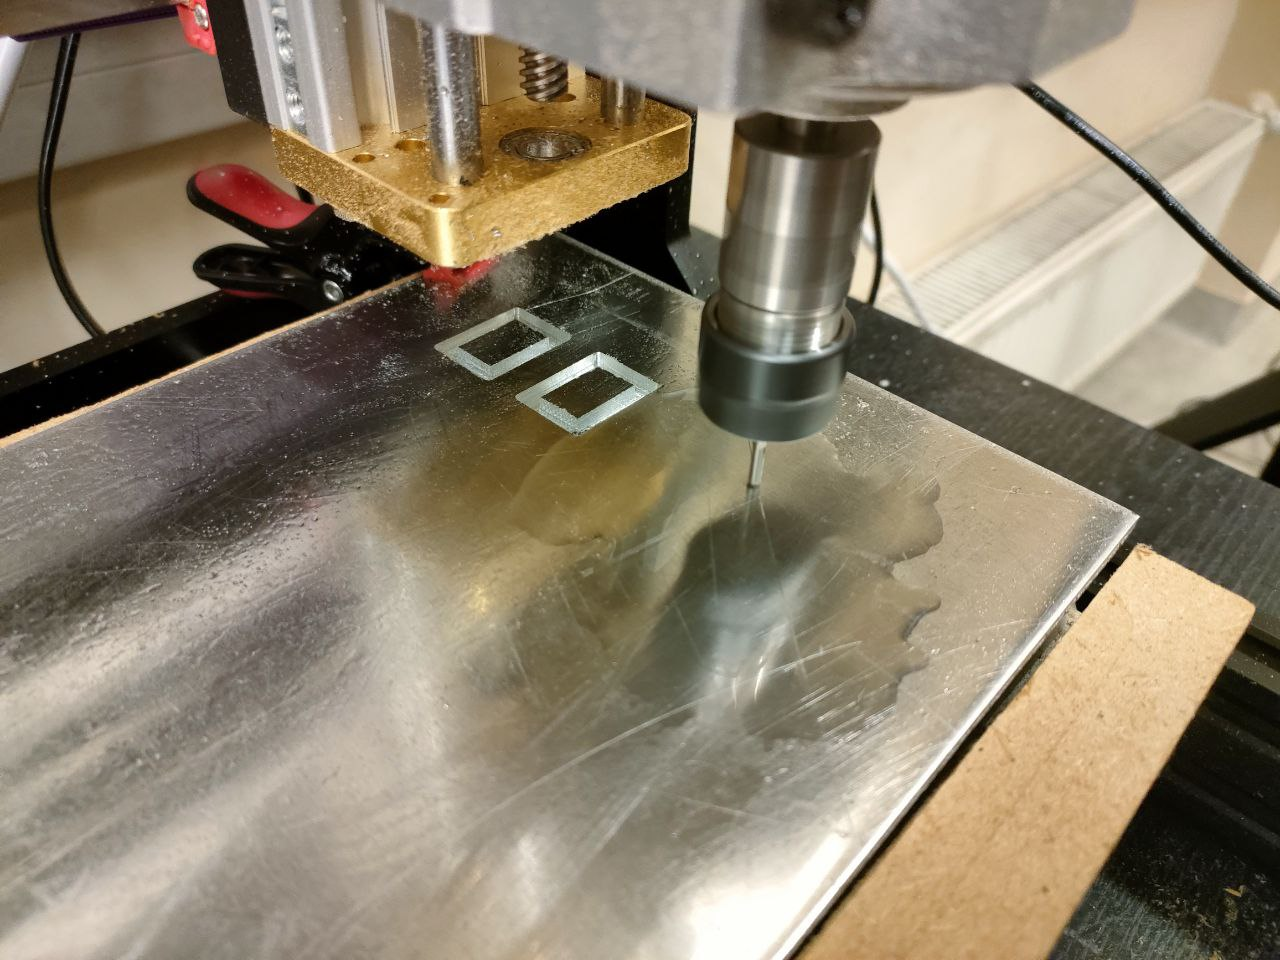
\includegraphics[width=7.5cm]{images/frezarka_3018.jpg} }}%
    \caption{Proces frezowania panelu frontowego.}
    \label{fig:ugs}%
\end{figure}

Pozostałe elementy wykonane zostały za pomocą druku 3D z materiału PLA, bądź ABS. Elementy te widoczne są na rysunku 
\ref{fig:druk3d}. Wśród nich znajdują się: narożniki obudowy, przyciski, gałka enkodera, mocowania wentylatorów, zasilacza 
24 V, płytek PCB oraz wyświetlacza. Elementy mocujące płytki PCB oraz trzymające kable łączone są ze sobą za pomocą śrub 
wkręcanych w mosiężne inserty gwintowane, wtapiane w elementy plastikowe.

\begin{figure}[h!]
    \begin{center}
        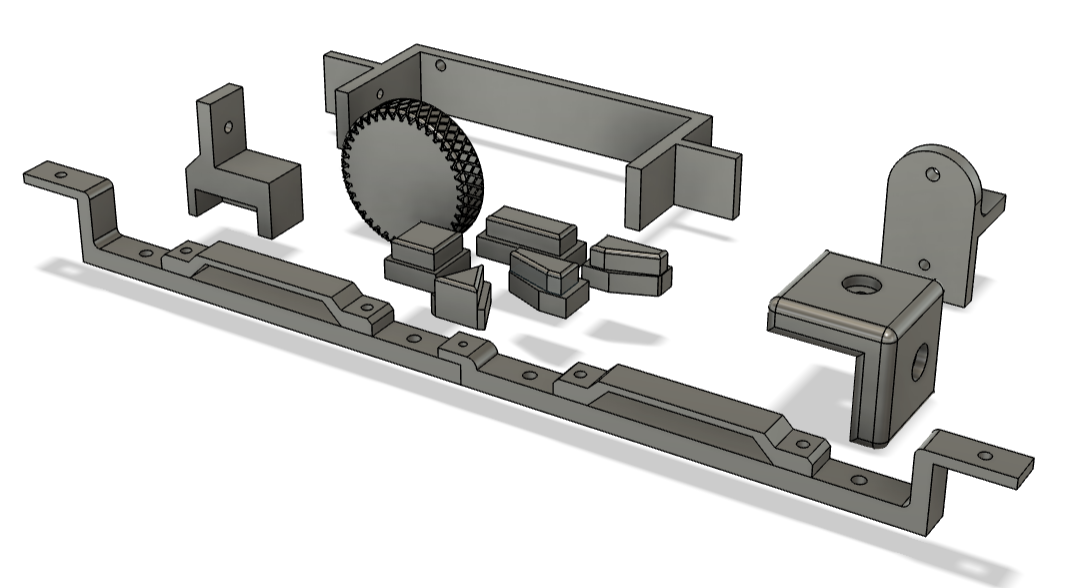
\includegraphics[width = 15cm]{images/druk3d.png}
        \caption{Elementy wykonane w technologii FDM.} 
        \label{fig:druk3d}
    \end{center}
\end{figure}

Kompletne złożone urządzenie przedstawiają zdjęcia \ref{fig:kompletne_urzadzenie} oraz \ref{fig:rzut_z_gory}.

\begin{figure}[h!]
    \begin{center}
        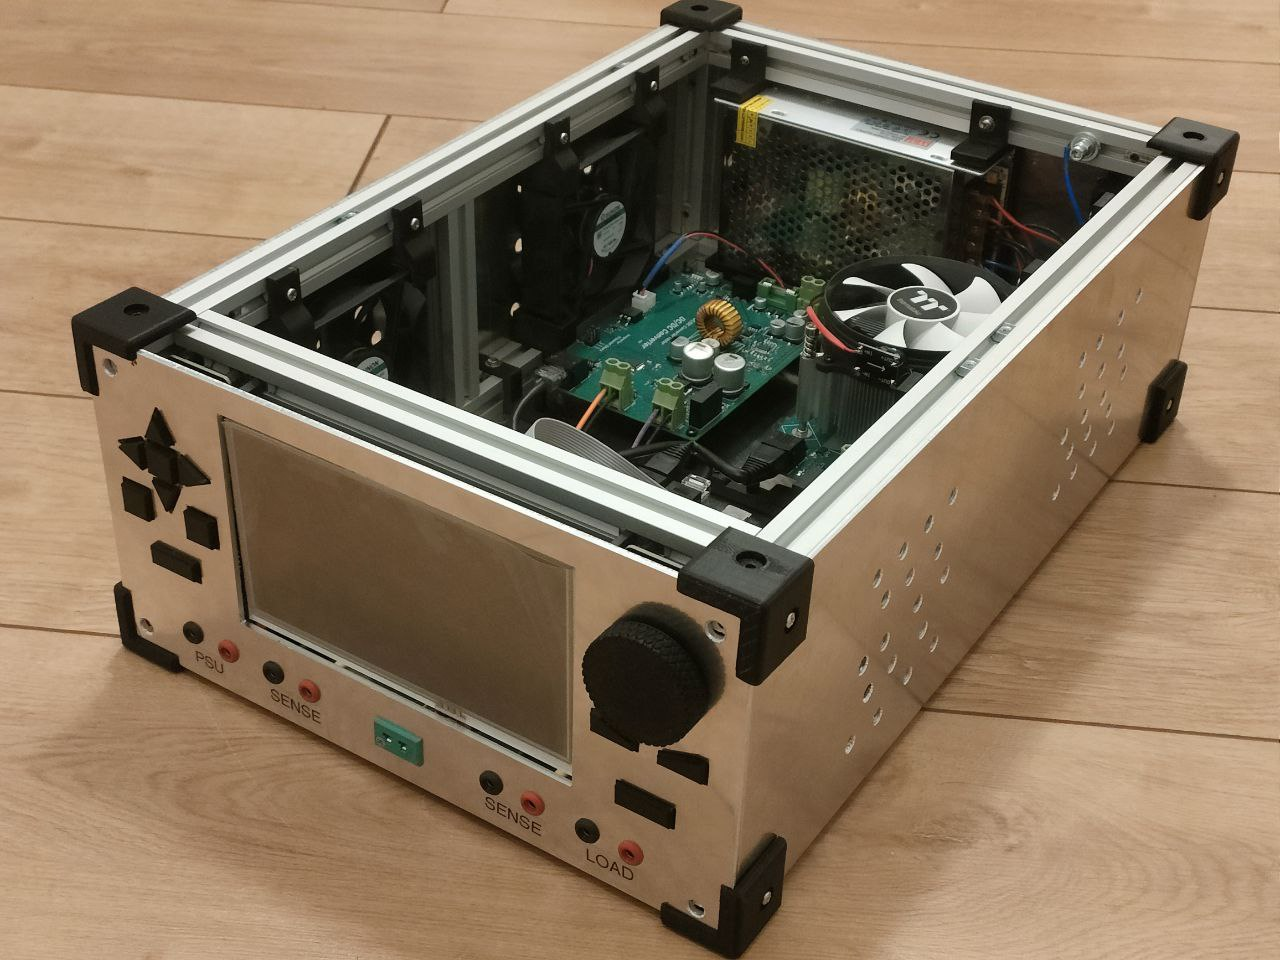
\includegraphics[width = 15cm]{images/zdjecie_kompletne.jpg}
        \caption{Zdjęcie kompletnego urządzenia bez górnej pokrywy.} 
        \label{fig:kompletne_urzadzenie}
    \end{center}
\end{figure}

\begin{figure}[h!]
    \begin{center}
        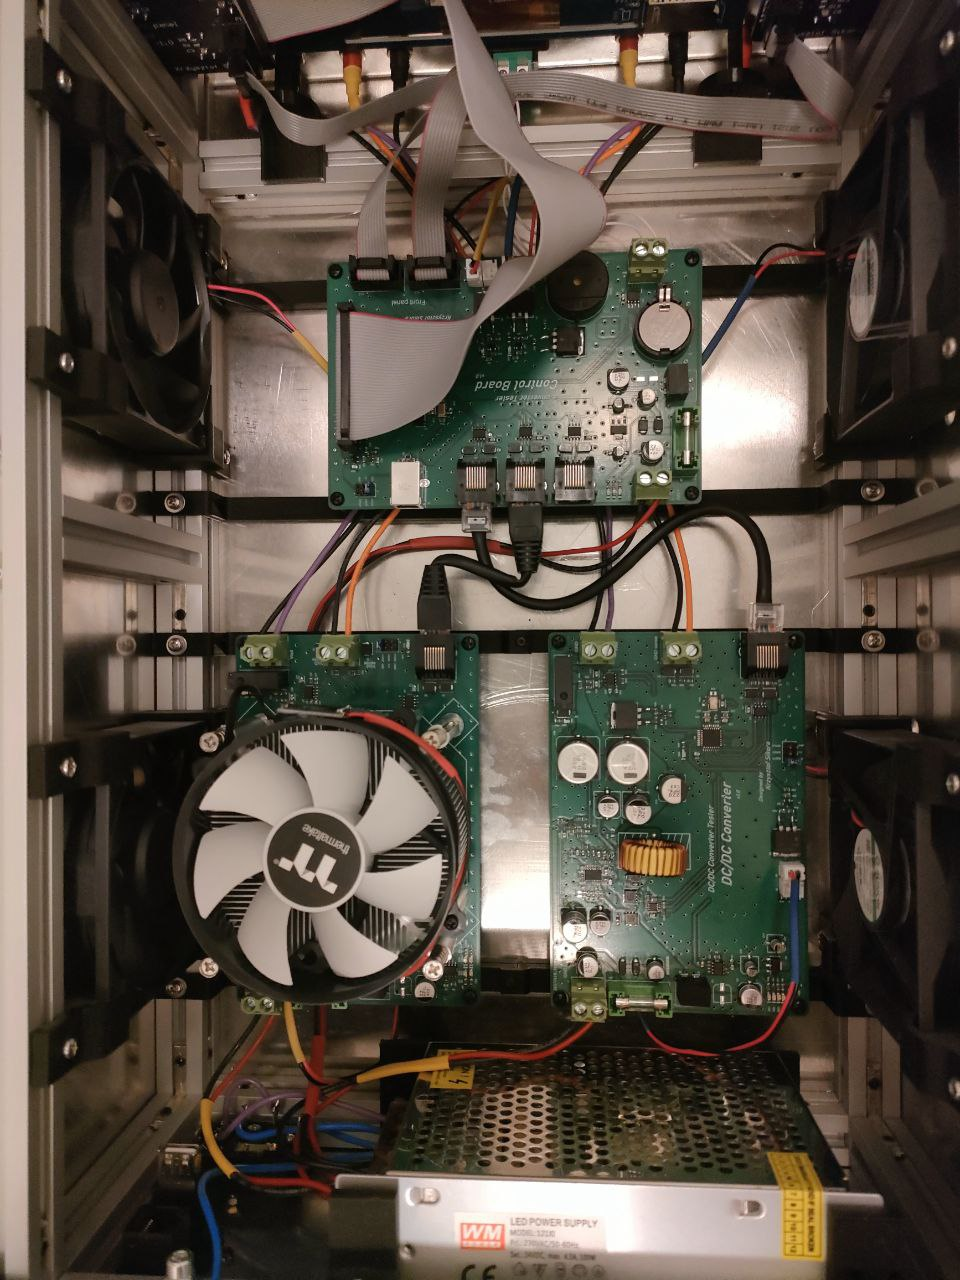
\includegraphics[angle=90, width = 15cm]{images/zdjecie_elektroniki.jpg}
        \caption{Widok urządzenia ze zmontowaną elektroniką.}
        \label{fig:rzut_z_gory}
    \end{center}
\end{figure}

Jako wyjścia oraz wejścia modułów zasilacza regulowanego i obciążenia aktywnego wykorzystano klasyczne złącza bananowe.
Pomiędzy nimi, na panelu frontowym znajduje się gniazdo termopary typu K, konkretnie model 4559742 od RS COMPONENTS \cite{ktypeconn}.
Styki złącza wykonane są z materiału odpowiedniego dla danego typu termopary, a kolor zgodny jest z normą IEC 60584-3.
Z tyłu obudowy znalazło się także miejsce na złącza panelowe: USB typu B oraz RJ45, które można podłączyć do modułu kontrolera.
Poniżej zamontowano złącze zasilania 230 V (wtyczka C14) z włącznikiem i bezpiecznikiem topikowym.

Zastosowane wentylatory to SUNON MF92252V3-A99-A, o wymiarach 92 mm x 92 mm i napięciu pracy 24 V. Ich wymiar umożliwił 
montaż bezpośrednio pomiędzy profilami aluminiowymi. W tylnej części obudowy widoczny jest główny zasilacz 24 V firmy Mean Well.
Odpowiada on za zasilanie wszystkich trzech modułów z elektroniką. Doprowadzenia do obudowy metalowej napięcia 230 V 
pociąga za sobą konieczność uziemienia obudowy, które wykonano przewodem połączonym z profilami aluminiowymi.

\chapter{Testy}
\label{chapter-5}

\vspace{0.5cm}

W rozdziale opisano kolejne etapy testowania urządzenia.

\FloatBarrier
\section{Testy}

Po złożeniu urządzenia przeprowadzono testy podstawowych funkcjonalności. Wyniki najważniejszych pomiarów przedstawiono 
w następnych podrozdziałach. Pomiary wartości prądu oraz napięcia dokonywane były multimetrami Uni-T UT60EU oraz UT107+.

\FloatBarrier
\subsection{Testy zasilacza regulowanego}

Przy pomocy zewnętrznego obciążenia aktywnego zweryfikowano działanie przetwornicy w module zasilacza regulowanego.
Zmierzono napięcie na wyjściu modułu dla trzech wybranych napięć (5 V, 9 V, 12 V, 15 V) oraz zakresu prądów od 0.1 A do 2 A. 
Zebrane dane przedstawiono w tabeli \ref{tab:pomiaryZasilacza}. Błąd względny obliczany jest ze wzoru: 
$\frac{V_{ustawione} - V_{zmierzone}}{V_{ustawione}} \cdot 100 \%$

\begin{table}[]
\centering
\begin{tabular}{|l|l|l|l|}
\hline
Napięcie ustawione {[}V{]} & Prąd wyjściowy {[}A{]} & Napięcie zmierzone {[}V{]} & Błąd względny {[}\%{]} \\ \hline
5                          & 0.1                    & 4.972                      & 0.56                   \\ \hline
5                          & 0.5                    & 4.94                       & 1.2                    \\ \hline
5                          & 1                      & 4.888                      & 2.24                   \\ \hline
5                          & 1.5                    & 4.832                      & 3.36                   \\ \hline
5                          & 2                      & 4.784                      & 4.32                   \\ \hline
9                          & 0.1                    & 8.992                      & 0.0889                 \\ \hline
9                          & 0.5                    & 8.956                      & 0.4889                 \\ \hline
9                          & 1                      & 8.904                      & 1.0667                 \\ \hline
9                          & 1.5                    & 8.848                      & 1.6889                 \\ \hline
9                          & 2                      & 8.802                      & 2.2                    \\ \hline
12                         & 0.1                    & 12.004                     & -0.0333                \\ \hline
12                         & 0.5                    & 11.965                     & 0.2917                 \\ \hline
12                         & 1                      & 11.916                     & 0.7                    \\ \hline
12                         & 1.5                    & 11.864                     & 1.1333                 \\ \hline
12                         & 2                      & 11.812                     & 1.5667                 \\ \hline
15                         & 0.1                    & 15.028                     & -0.1867                \\ \hline
15                         & 0.5                    & 14.998                     & 0.0133                 \\ \hline
15                         & 1                      & 14.936                     & 0.4267                 \\ \hline
15                         & 1.5                    & 14.888                     & 0.7467                 \\ \hline
15                         & 2                      & 14.852                     & 0.9867                 \\ \hline
\end{tabular}
\caption{Wyniki pomiarów modułu zasilacza regulowanego.}
\label{tab:pomiaryZasilacza}
\end{table}


\subsection{Testy obciążenia aktywnego}

Pomiary działania modułu obciążenia aktywnego wykonywano korzystając z zewnętrznego zasilacza laboratoryjnego PS-305D YIHUA.
Napięcie na zasilaczu ustawiono na 6 V oraz 12 V. Zmierzono pobierany przez moduł prąd dla kilku ustalonych wartości.
Zmierzone wartości przedstawia tabela \ref{tab:pomiaryObciazenia}. Błąd względny obliczany jest ze wzoru: 
$\frac{I_{ustawione} - I_{zmierzone}}{I_{ustawione}} \cdot 100 \%$
\begin{table}[]
\centering
\begin{tabular}{|l|l|l|l|}
\hline
Napięcie zasilacza {[}V{]} & Prąd ustawiony {[}A{]} & Prąd zmierzony {[}A{]} & Błąd względny {[}\%{]} \\ \hline
12                         & 0.1                    & 0.0994                 & 0.6                    \\ \hline
12                         & 0.5                    & 0.4945                 & 1.1                    \\ \hline
12                         & 1                      & 1.022                  & -2.2                   \\ \hline
12                         & 1.5                    & 1.514                  & -0.93333               \\ \hline
12                         & 2                      & 1.981                  & 0.95                   \\ \hline
6                          & 0.1                    & 0.0987                 & 1.3                    \\ \hline
6                          & 0.5                    & 0.4889                 & 2.22                   \\ \hline
6                          & 1                      & 1.001                  & -0.1                   \\ \hline
6                          & 1.5                    & 1.503                  & -0.2                   \\ \hline
6                          & 2                      & 1.992                  & 0.4                    \\ \hline
\end{tabular}
\caption{Wyniki pomiarów modułu obciążenia aktywnego.}
\label{tab:pomiaryObciazenia}
\end{table}



\subsection{Pomiar prądu i napięcia}

Sprawdzono również dokładność pomiaru prądu oraz napięcia, które dokonywane są w obu modułach poprzez układ INA219.
Wykorzystano w tym celu moduł zasilacza regulowanego do ustalania napięcia wyjściowego do pomiaru napięcia oraz 
moduł obciążenia aktywnego, w celu sprawdzenia dokładności pomiaru prądu. Tabele \ref{tab:pomiaryINA219} oraz 
\ref{tab:pomiaryINA2192} zawierają wyniki wykonanych pomiarów. Błąd względny liczony był analogicznie 
do pomiarów przedstawionych wcześniej.


\begin{table}[]
\centering
\begin{tabular}{|l|l|l|}
\hline
Napięcie zmierzone {[}V{]} & Napięcie rzeczywiste {[}V{]} & Błąd względny   {[}\%{]} \\ \hline
2.968                      & 2.978                        & -0.336             \\ \hline
4.988                      & 4.986                        & 0.040              \\ \hline
7.992                      & 8.001                        & -0.112             \\ \hline
11.004                     & 11.01                        & -0.054             \\ \hline
15.028                     & 15.05                        & -0.146             \\ \hline
19.04                      & 19.06                        & -0.105             \\ \hline
\end{tabular}
\caption{Pomiar napięcia przy pomocy układu INA219 oraz multimetru.}
\label{tab:pomiaryINA219}
\end{table}

\begin{table}[]
\centering
\begin{tabular}{|l|l|l|}
\hline
Prąd   zmierzony {[}A{]} & Prąd rzeczywisty   {[}A{]} & Błąd względny   {[}\%{]} \\ \hline
0.124                    & 0.121                      & 2.419              \\ \hline
0.241                    & 0.238                      & 1.244              \\ \hline
0.4                      & 0.399                      & 0.250                     \\ \hline
0.544                    & 0.541                      & 0.551              \\ \hline
0.841                    & 0.836                      & 0.594              \\ \hline
1.048                    & 1.042                      & 0.572              \\ \hline
1.267                    & 1.259                      & 0.631              \\ \hline
1.58                     & 1.567                      & 0.822               \\ \hline
1.812                    & 1.781                      & 1.710              \\ \hline
2.052                    & 2.01                       & 2.046             \\ \hline
\end{tabular}
\caption{Pomiar prądu przy pomocy układu INA219 oraz multimetru.}
\label{tab:pomiaryINA2192}
\end{table}




\subsection{Automatyczny pomiar sprawności przetwornicy}

Jednym z głównych celów projektu, jakie przedstawione zostały na początku tej pracy, była automatyzacja pomiaru sprawności 
przetwornic napięciowych. W tym celu, wytworzone oprogramowanie pozwala na wybór napięcia wejściowego oraz zakresu prądów obciążenia
przetwornicy. Następnie, po podłączeniu badanego układu (DUT), załączany jest moduł zasilacza regulowanego i ustalane napięcie wejściowe.
Obciążenie aktywne ustala następnie prąd wyjściowy DUT i oba moduły mierzą moc na swoich wejściach, tj. napięcie oraz prąd.
Po wykonaniu pomiaru, liczona jest sprawność, czyli stosunek mocy wejściowej i wyjściowej. Proces ten wykonywany jest dla
całego zakresu prądu obciążenia z wybranym krokiem. Po zakończeniu pomiarów, na wyświetlaczu urządzenia widoczny jest wykres
sprawności w podanym zakresie prądu obciążenia. Przykładowy wykonywany pomiar przedstawia zdjęcie \ref{fig:pomiarsprawnosci}.

\begin{figure}[h!]
    \begin{center}
        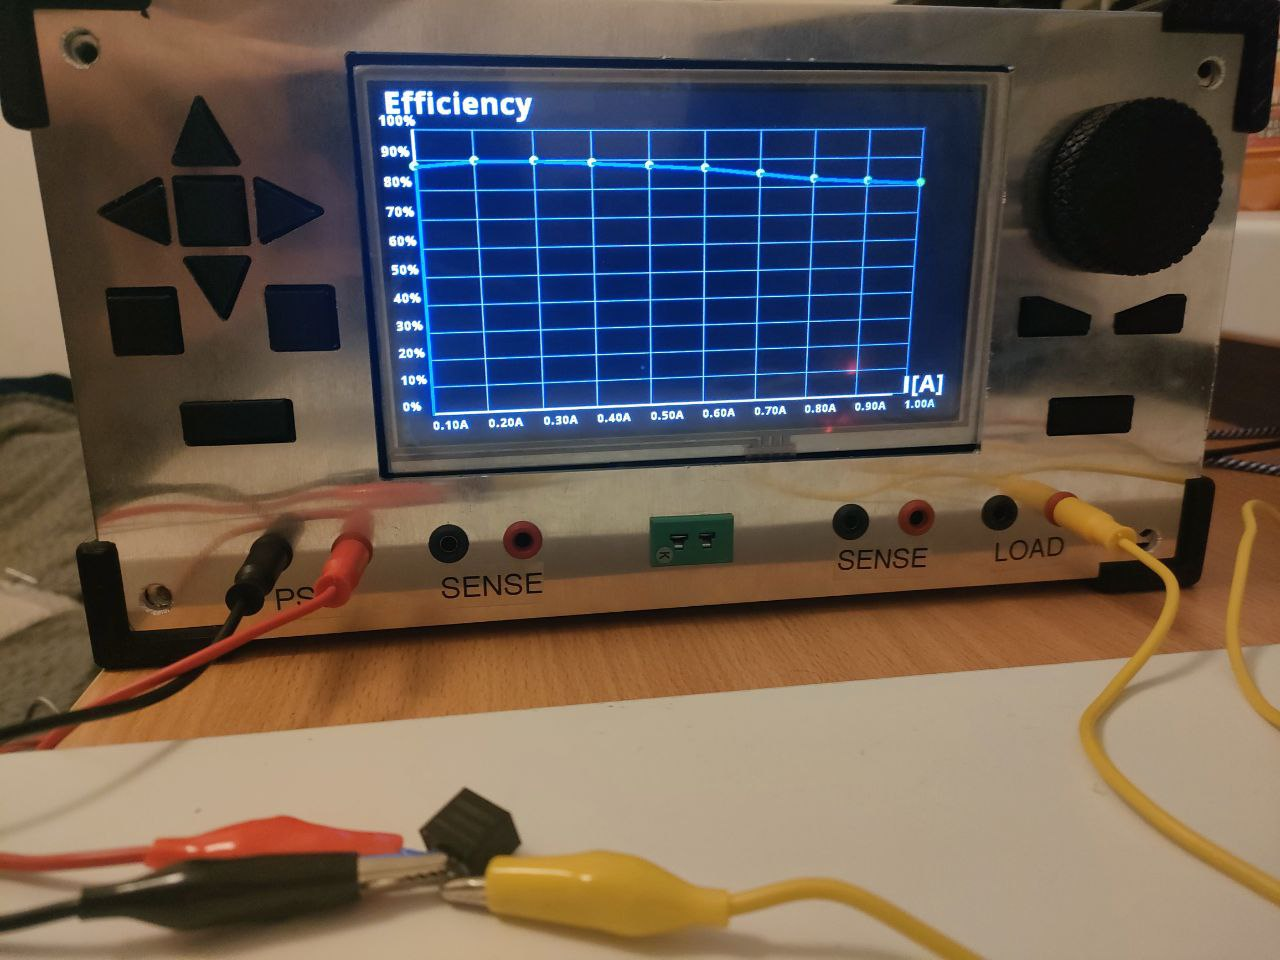
\includegraphics[width = 15cm]{images/pomiarSprawnosci.jpg}
        \caption{Automatyczny pomiar sprawności podłączonej przetwornicy.}
        \label{fig:pomiarsprawnosci}
    \end{center}
\end{figure}

Na zdjęciu widoczna jest przetwornica MORNSUN K7805-500R3 \cite{MORNSUN}. Jej napięcie wyjściowe to 5 V, natomiast maksymalny 
prąd to 500 mA. Pomiar wykonany został dla zakresu 0.1 A do 1 A, z krokiem 100 mA. Wartość 1 A przekracza oczywiście 
maksimum podane przez producenta, lecz testy wykazały stabilną pracę w temperaturze pokojowej do ponad 1 A, przy spadku 
napięcia wyjściowego do 4.4 V. Gwarantowany zakres 500 mA zakłada, że napięcie wyjściowe mieści się w zakresie 4\% od 
ustalonej wartości. 

Wykres \ref{fig:sprawnoscZmierzona} wygenerowany został z pomiarów w zakresie 0.05 A do 0.5 A prądu obciążenia, przy zasilaniu 
z napięcia 9 V.
Jest on analogiczny do wykresy przedstawionego na rysunku \ref{fig:sprawnoscOdProducenta}.

\begin{figure}[h!]
    \begin{center}
        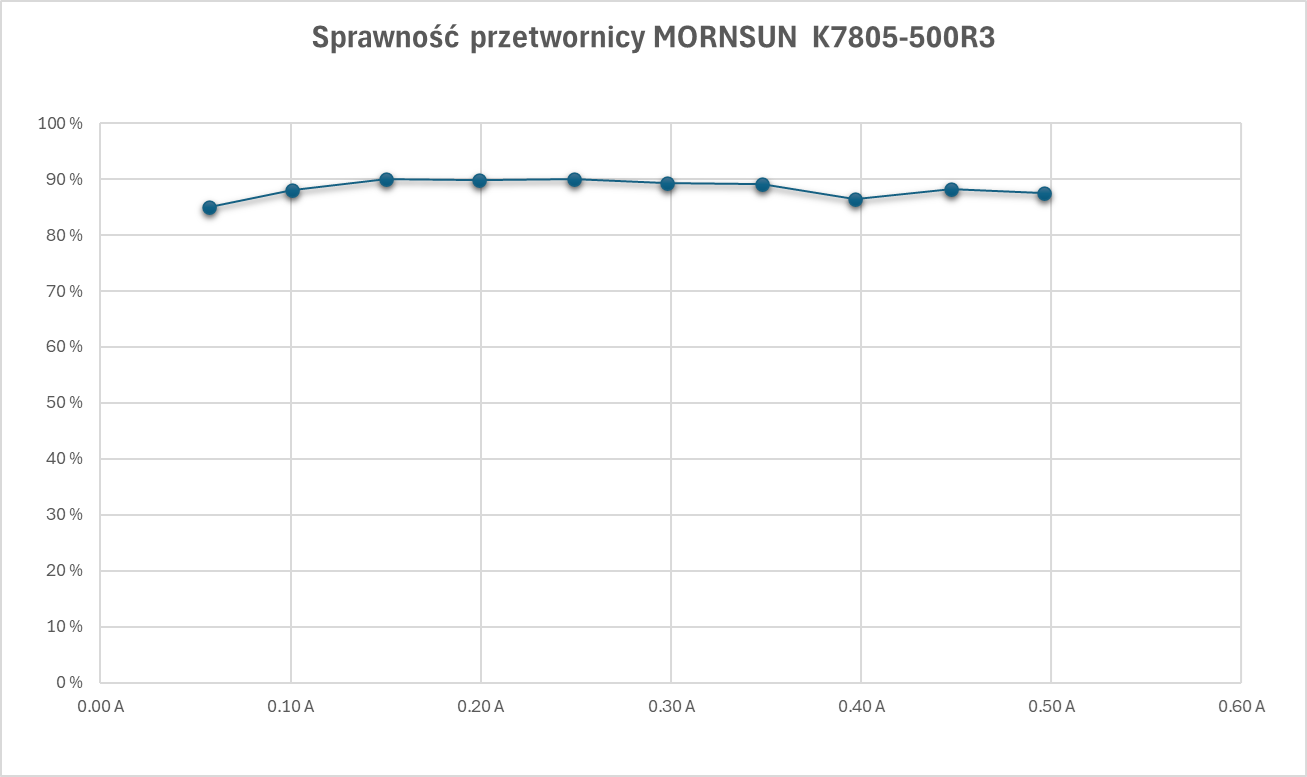
\includegraphics[width = 15cm]{images/sprawnoscZmierzonaMORNSUN.png}
        \caption{Wykres powstały ze zmierzonych wartości mocy przetwornicy MORNSUN.}
        \label{fig:sprawnoscZmierzona}
    \end{center}
\end{figure}

\begin{figure}[h!]
    \begin{center}
        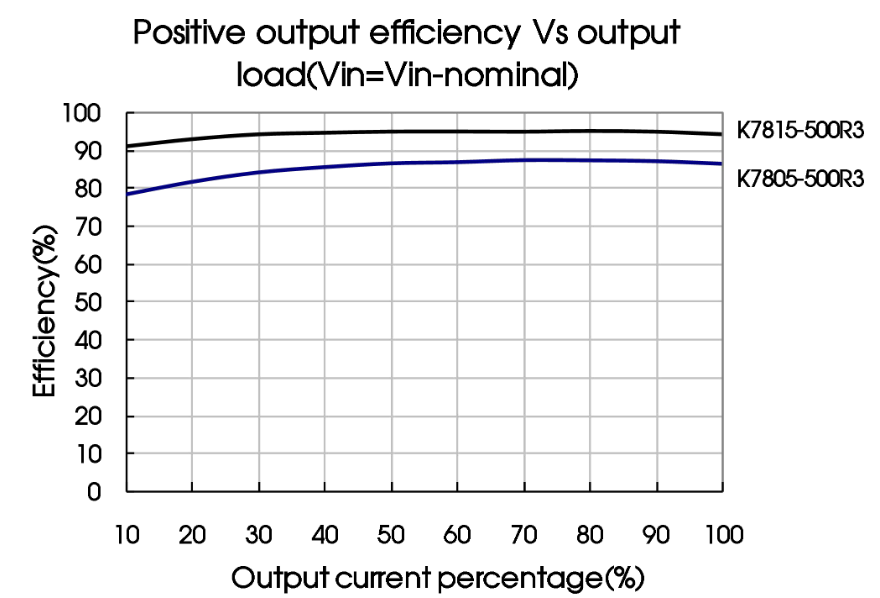
\includegraphics[width = 15cm]{images/sprawnoscProducentMORNSUN.png}
        \caption{Wykres sprawności przetwornicy MORNSUN z dokumentacji producenta.}
        \label{fig:sprawnoscOdProducenta}
    \end{center}
\end{figure}

Zarówno wykres z dokumentacji producenta, jak i wygenerowany z pomiarów, przedstawiają podobną krzywą sprawności.
Dla niewielkiego prądu wyjściowego sprawność wynosi około 85\% i wzrasta do prawie 90\% w połowie zakresu, po czym utrzymuje
ten poziom, aż do pełnego zakresu 500 mA.



\FloatBarrier
\chapter{Podsumowanie}
\label{chapter-6}

Celem niniejszej pracy było zaprojektowanie i wykonanie modułowego urządzenia, umożliwiającego automatyzację pomiarów 
przetwornic napięciowych (DC/DC). W tym celu konieczne było zaprojektowanie zasilacza regulowanego, obciążenia aktywnego
oraz kontrolera, przy pomocy którego możliwe byłoby zarządzanie innymi modułami.
Moduły te zostały wykonane, a następnie przetestowane. Stwierdzono poprawne działanie wszystkich elementów oraz zadowalającą
dokładność stworzonego sprzętu. 

Automatyczny pomiar sprawności przetwornicy wykorzystywany był wielokrotnie z pozytywnym wynikiem i znacząco przyspieszał
proces. Napisane oprogramowanie ocenione zostało przez osoby testujące jako responsywne i proste w użyciu. 
Wykonanie stosownej obudowy z odpornych materiałów, oraz przemyślany interfejs zapewniają sprawne działanie bez obaw 
o ewentualne uszkodzenia czy awarie.
Zrealizowany projekt inżynierski wykorzystuje wiele elementów, które wybrane zostały przez autora pracy z myślą o dalszym rozwoju
i potencjalnym modyfikacjom. W ramach tego, możliwe jest dodanie dodatkowych funkcjonalności automatycznego pomiaru innych 
parametrów przetwornic, czy też innych urządzeń, np.: pomiar pojemności akumulatorów, pomiar rezystancji przewodów metodą
Kelvina.
 

\begin{thebibliography}{}

\bibitem{przetworncieNapieciowe} Przetwornice napięciowe, \url{https://pl.wikipedia.org/wiki/Przetwornica_napi%C4%99cia}, dostęp 01.11.2024 r.

\bibitem{zasilaczeImpulsowe} Zasilacze impulsowe, \url{https://pl.wikipedia.org/wiki/Zasilacz_impulsowy}, dostęp 01.11.2024 r.

\bibitem{typyPrzetwornic} Przetwornica buck-boost, \url{https://en.wikipedia.org/wiki/Buck%E2%80%93boost_converter}, dostęp 01.11.2024 r.

\bibitem{spice} SPICE, \url{https://en.wikipedia.org/wiki/SPICE}, dostęp 01.11.2024 r.

\bibitem{przetwornicaOmniON} Moduł przetwornicy OmniON, \url{https://www.mouser.it/new/omnion-power/omnion-power-qsxw050a0b-dc-dc-modules/}, dostęp 01.11.2024 r.

\bibitem{altiumDesigner} Altium Designer, \url{https://www.altium.com/altium-designer}, dostęp 01.11.2024 r.

\bibitem{stm32f401} Datasheet STM32F401VET6, \url{https://www.st.com/content/ccc/resource/technical/document/datasheet/30/91/86/2d/db/94/4a/d6/DM00102166.pdf/files/DM00102166.pdf/jcr:content/translations/en.DM00102166.pdf}, dostęp 01.11.2024 r.

\bibitem{RS485} Opis interfejsu RS485, \url{https://www.ccontrols.com/pdf/ExtV1N1.pdf}, dostęp 01.11.2024 r.

\bibitem{MAX3485} Datasheet MAX3485, \url{https://www.analog.com/media/cn/technical-documentation/data-sheets/1079.pdf}, dostęp 09.11.2024 r.

\bibitem{napieciaRS} Standardy RS422/RS485, \url{https://www.delock.com/infothek/RS-422_RS-485/RS-422_RS-485_e.html}, dostęp 01.11.2024 r.

\bibitem{SSD1963} Kontroler SSD1963, \url{https://ww1.microchip.com/downloads/en/DeviceDoc/SSD1963_LCD_Controller_%20Graphics_Card_DS50002915A.pdf}, dostęp 01.11.2024 r.

\bibitem{termopara} Termopara, \url{https://pl.wikipedia.org/wiki/Termopara}, dostęp 01.11.2024 r.

\bibitem{max6675} Datasheet MAX6675, \url{https://www.analog.com/media/en/technical-documentation/data-sheets/MAX6675.pdf}, dostęp 01.11.2024 r.

\bibitem{termoparaSeebeck} Zjawisko Seebecka, \url{https://www.techtarget.com/searchnetworking/definition/Seebeck-effect}, dostęp 01.11.2024 r.

\bibitem{AMSRI1} Dokumentacja AMSRI1, \url{http://www.aimtec.com/site/Aimtec/files/Datasheet/HighResolution/amsr1-z.pdf}, dostęp 09.11.2024 r.

\bibitem{TLV76133} Dokumentacja LDO TLV76133, \url{https://www.ti.com/lit/ds/symlink/tlv761.pdf}, dostęp 09.11.2024 r.

\bibitem{MP9928} Dokumentacja układu przetwornicy MP9928, \url{https://www.monolithicpower.com/en/documentview/productdocument/index/version/2/document_type/Datasheet/lang/en/sku/MP9928/?srsltid=AfmBOoq7GuS46Yk88IgI9IL9-YGCLxkan8e_ik8h-mNoc0YwlZz8QCuL}, dostęp 09.11.2024 r.

\bibitem{obliczaniePojemnosciBuck} Basic Calculation of a Buck Converter's Power Stage, \url{https://www.ti.com/lit/an/slva477b/slva477b.pdf?ts=1733342064235&ref_url=https%253A%252F%252Fwww.google.com%252F}, dostęp 05.12.2024 r.

\bibitem{SQJ850EP} Dokumentacja tranzystora SQJ850EP, \url{https://www.vishay.com/docs/65280/sqj850ep.pdf}, dostęp 09.11.2024 r.

\bibitem{evalboardMP9928} Płytka ewaluacyjna MP9928, \url{https://www.monolithicpower.com/en/documentview/productdocument/index/version/2/document_type/Datasheet/lang/en/sku/EV9928-F-00B/document_id/3375/}, dostęp 09.11.2024 r.

\bibitem{mpsmart} Oprogramowanie MPSmart, \url{https://www.monolithicpower.com/en/mpsmart-v9.html?srsltid=AfmBOop79kl3gR7Ojs1PbaIpAlMgfDhco18PwP2i3f6T2zJfTZ_qEZrz}, dostęp 09.11.2024 r.

\bibitem{fundamentalsofpowerelectronics} Fundamentals Of Power Electronics, autorzy:  Robert W. Erickson , Dragan Maksimović, wydanie 2020

\bibitem{variableoutput} How to Design a Variable Output Buck Regulator, \url{https://www.analog.com/jp/resources/technical-articles/a-3step-approach-for-designing-a-variable-output-buck-regulator.html}, dostęp 10.11.2024 r.

\bibitem{n6705c} Keysight N6705C, \url{https://www.keysight.com/us/en/product/N6705C/dc-power-analyzer-modular-600-w-4-slots.html}, dostęp 12.10.2024 r.

\bibitem{ina219} Dokumentacja układu pomiaru prądu i napięcia INA219, \url{https://www.ti.com/lit/ds/symlink/ina219.pdf?ts=1731224153420&ref_url=https%253A%252F%252Fwww.google.com%252F}, dostęp 10.11.2024 r.

\bibitem{stm32f303} Dokumentacja mikrokontrolera STM32F303K8T6, \url{https://www.st.com/resource/en/datasheet/stm32f303k8.pdf}, dostęp 10.11.2024 r.

\bibitem{lt1461} Dokumentacja układu LT1461CC, \url{https://www.analog.com/media/en/technical-documentation/data-sheets/LT1461.pdf}, dostęp 10.11.2024 r.

\bibitem{jlcpcb} Producent płytek PCB - JLCPCB, \url{https://jlcpcb.com/}, dostęp 10.11.2024 r.

\bibitem{IRFP240} Dokumentacja MOSFET typu N - IRFP240, \url{https://www.vishay.com/docs/91210/irfp240.pdf}, dostęp 10.11.2024 r.

\bibitem{parallelMOS} Nota aplikacyjna AND8199/D, \url{https://www.onsemi.cn/PowerSolutions/document/AND8199-D.PDF}, dostęp 10.11.2024 r.

\bibitem{RA-T2X-51E} Dokumentacja radiatora RA-T2X-51E, \url{https://www.tme.eu/Document/ad1db061b7bf4b6eae656461c3bb5f61/RA-T2X-51E.pdf}, dostęp 10.11.2024 r.

\bibitem{thermaltake} Radiator thermaltake gravity i3, \url{https://www.thermaltake.com/gravity-i3.html}, dostęp 10.11.2024 r.

\bibitem{bidirectional_DC_PSU} ElektroAutomatik, \url{https://elektroautomatik.com/en/products/dc-bidirectional-power-supplies/}, dostęp 12.10.2024 r.

\bibitem{SSD1963_DRIVER} Biblioteka drivera do SSD1963, \url{https://github.com/offpic/7-SSD1963-GPIO-HIGH-SPEED-STM32-STM32F401-GAUGE}, dostęp 12.10.2024 r.

\bibitem{fusion360} Oprogramowanie fusion360, \url{https://www.autodesk.com/products/fusion-360}, dostęp 22.12.2024 r.

\bibitem{ktypeconn} Złącze termopary RS COMPONENTS, \url{https://pl.rs-online.com/web/p/akcesoria-do-czujnikow/4559742?srsltid=AfmBOooj4xmu6XScA-BCboP2SBJIe7dSX3QR98rF_B7sTZLFJNxZeTKQ}, dostęp 22.12.2024 r.

\bibitem{MORNSUN} Dokumentacja przetwornicy MORNSUN k7805-500r3, \url{https://www.mornsun-power.com/html/pdf/K7805-500R3.html}, dostęp 22.12.2024 r.

\bibitem{python} Python, \url{https://www.python.org/}, dostęp 12.10.2024 r.

\bibitem{labview} LabView, \url{https://www.ni.com/en/shop/labview.html}, dostęp 12.10.2024 r.

\end{thebibliography}


\appendix
%\newgeometry{left=1cm, right=1cm, bottom=1cm, top=1cm}

\chapter{Moduł kontrolera}
\begingroup
\renewcommand{\cleardoublepage}{}
\renewcommand{\clearpage}{}
\begin{figure}[h!]
    \begin{center}
        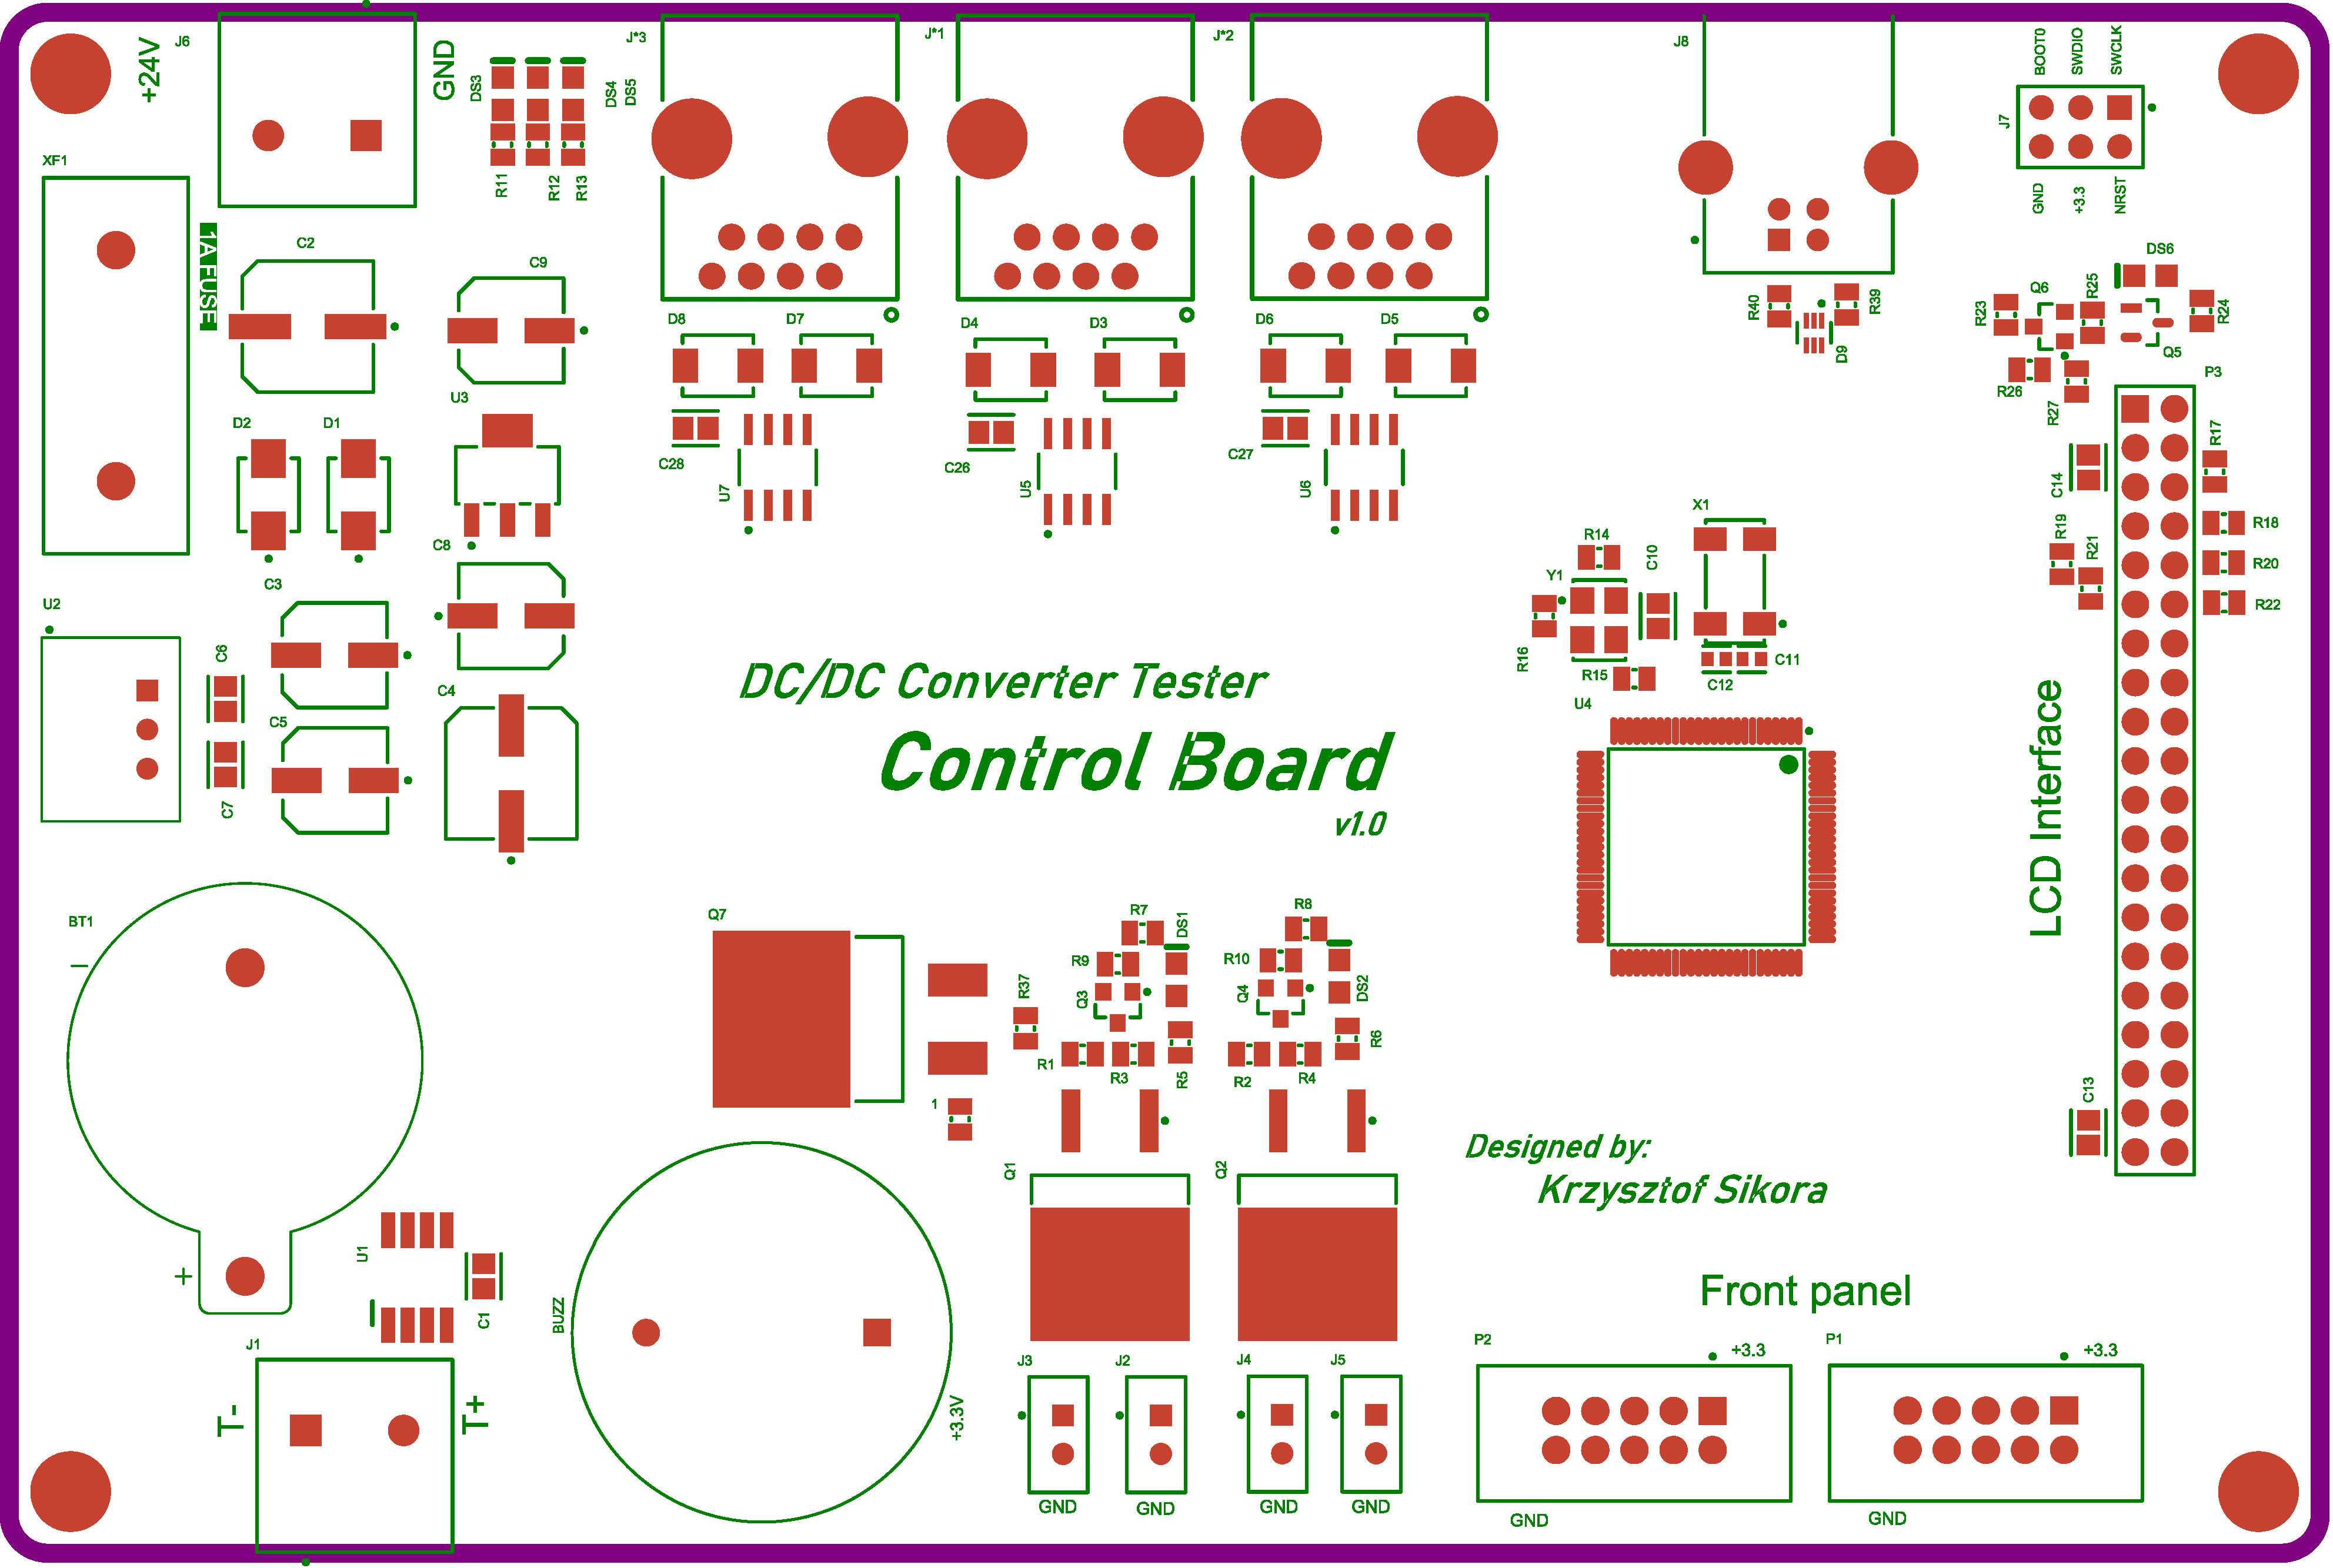
\includegraphics[width = 17cm]{zalaczniki/kontroler/Kontroler_Strona_15.jpg}
        \caption{Widok warstwy opisowej PCB.}
    \end{center}
\end{figure}

\begin{sidewaysfigure}
    \begin{center}
        \includegraphics[width = 21cm]{zalaczniki/kontroler/Kontroler_Strona_01.jpg}
        \caption{Schemat blokowy modułu kontrolera.}
    \end{center}
\end{sidewaysfigure}

\begin{sidewaysfigure}
    \begin{center}
        \includegraphics[width = 21cm]{zalaczniki/kontroler/Kontroler_Strona_02.jpg}
        \caption{Schemat układu termopary.}
    \end{center}
\end{sidewaysfigure}

\begin{sidewaysfigure}
    \begin{center}
        \includegraphics[width = 21cm]{zalaczniki/kontroler/Kontroler_Strona_03.jpg}
        \caption{Schemat kontrolera wentylatorów.}
    \end{center}
\end{sidewaysfigure}

\begin{sidewaysfigure}
    \begin{center}
        \includegraphics[width = 21cm]{zalaczniki/kontroler/Kontroler_Strona_04.jpg}
        \caption{Schemat sekcji zasilania.}
    \end{center}
\end{sidewaysfigure}

\begin{sidewaysfigure}
    \begin{center}
        \includegraphics[width = 21cm]{zalaczniki/kontroler/Kontroler_Strona_05.jpg}
        \caption{Schemat układów oscylatorów.}
    \end{center}
\end{sidewaysfigure}

\begin{sidewaysfigure}
    \begin{center}
        \includegraphics[width = 21cm]{zalaczniki/kontroler/Kontroler_Strona_06.jpg}
        \caption{Schemat wyprowadzeń przycisków.}
    \end{center}
\end{sidewaysfigure}

\begin{sidewaysfigure}
    \begin{center}
        \includegraphics[width = 21cm]{zalaczniki/kontroler/Kontroler_Strona_07.jpg}
        \caption{Schemat wyprowadzania LCD.}
    \end{center}
\end{sidewaysfigure}

\begin{sidewaysfigure}
    \begin{center}
        \includegraphics[width = 21cm]{zalaczniki/kontroler/Kontroler_Strona_08.jpg}
        \caption{Schemat mikrokontrolera STM32.}
    \end{center}
\end{sidewaysfigure}

\begin{sidewaysfigure}
    \begin{center}
        \includegraphics[width = 21cm]{zalaczniki/kontroler/Kontroler_Strona_09.jpg}
        \caption{Schemat RS485.}
    \end{center}
\end{sidewaysfigure}

\begin{sidewaysfigure}
    \begin{center}
        \includegraphics[width = 21cm]{zalaczniki/kontroler/Kontroler_Strona_10.jpg}
        \caption{Schemat układów peryferyjnych.}
    \end{center}
\end{sidewaysfigure}

\begin{figure}
    \begin{center}
        \includegraphics[width = 15cm]{zalaczniki/kontroler/Kontroler_Strona_11.jpg}
        \caption{Warstwa górna PCB.}
    \end{center}
\end{figure}

\begin{figure}
    \begin{center}
        \includegraphics[width = 15cm]{zalaczniki/kontroler/Kontroler_Strona_12.jpg}
        \caption{Warstwa wewnętrzna 1 PCB.}
    \end{center}
\end{figure}

\begin{figure}
    \begin{center}
        \includegraphics[width = 15cm]{zalaczniki/kontroler/Kontroler_Strona_13.jpg}
        \caption{Warstwa wewnętrzna 2 PCB.}
    \end{center}
\end{figure}

\begin{figure}
    \begin{center}
        \includegraphics[width = 15cm]{zalaczniki/kontroler/Kontroler_Strona_14.jpg}
        \caption{Warstwa dolna PCB.}
    \end{center}
\end{figure}



\nopagebreak

\chapter{Moduł zasilacza regulowanego}


\begin{figure}[h!]
    \begin{center}
        \includegraphics[width = 17cm]{zalaczniki/zasilacz/Zasilacz_regulowany_Strona_13.jpg}
        \caption{Widok warstwy opisowej PCB.}
    \end{center}
\end{figure}

\begin{sidewaysfigure}
    \begin{center}
        \includegraphics[width = 21cm]{zalaczniki/zasilacz/Zasilacz_regulowany_Strona_01.jpg}
        \caption{Schemat blokowy modułu zasilacza.}
    \end{center}
\end{sidewaysfigure}

\begin{sidewaysfigure}
    \begin{center}
        \includegraphics[width = 21cm]{zalaczniki/zasilacz/Zasilacz_regulowany_Strona_02.jpg}
        \caption{Schemat RS485.}
    \end{center}
\end{sidewaysfigure}

\begin{sidewaysfigure}
    \begin{center}
        \includegraphics[width = 21cm]{zalaczniki/zasilacz/Zasilacz_regulowany_Strona_03.jpg}
        \caption{Schemat sekcji zasilania.}
    \end{center}
\end{sidewaysfigure}

\begin{sidewaysfigure}
    \begin{center}
        \includegraphics[width = 21cm]{zalaczniki/zasilacz/Zasilacz_regulowany_Strona_04.jpg}
        \caption{Schemat przetwornicy MP9928.}
    \end{center}
\end{sidewaysfigure}

\begin{sidewaysfigure}
    \begin{center}
        \includegraphics[width = 21cm]{zalaczniki/zasilacz/Zasilacz_regulowany_Strona_05.jpg}
        \caption{Schemat ukladu pomiaru prądu.}
    \end{center}
\end{sidewaysfigure}

\begin{sidewaysfigure}
    \begin{center}
        \includegraphics[width = 21cm]{zalaczniki/zasilacz/Zasilacz_regulowany_Strona_06.jpg}
        \caption{Schemat mikrokontrolera STM32.}
    \end{center}
\end{sidewaysfigure}

\begin{sidewaysfigure}
    \begin{center}
        \includegraphics[width = 21cm]{zalaczniki/zasilacz/Zasilacz_regulowany_Strona_07.jpg}
        \caption{Schemat sterownika wentylatorów.}
    \end{center}
\end{sidewaysfigure}

\begin{sidewaysfigure}
    \begin{center}
        \includegraphics[width = 21cm]{zalaczniki/zasilacz/Zasilacz_regulowany_Strona_08.jpg}
        \caption{Schemat układów peryferyjnych.}
    \end{center}
\end{sidewaysfigure}

\begin{figure}
    \begin{center}
        \includegraphics[width = 15cm]{zalaczniki/zasilacz/Zasilacz_regulowany_Strona_09.jpg}
        \caption{Warstwa górna PCB.}
    \end{center}
\end{figure}

\begin{figure}
    \begin{center}
        \includegraphics[width = 15cm]{zalaczniki/zasilacz/Zasilacz_regulowany_Strona_10.jpg}
        \caption{Warstwa wewnętrzna 2 PCB.}
    \end{center}
\end{figure}

\begin{figure}
    \begin{center}
        \includegraphics[width = 15cm]{zalaczniki/zasilacz/Zasilacz_regulowany_Strona_11.jpg}
        \caption{Warstwa wewnętrzna 2 PCB.}
    \end{center}
\end{figure}

\begin{figure}
    \begin{center}
        \includegraphics[width = 15cm]{zalaczniki/zasilacz/Zasilacz_regulowany_Strona_12.jpg}
        \caption{Warstwa dolna PCB.}
    \end{center}
\end{figure}


\nopagebreak

\chapter{Moduł obciążenia aktywnego}


\begin{figure}[h!]
    \begin{center}
        \includegraphics[width = 17cm]{zalaczniki/obciazenie/Obciążenie_aktywne_Strona_13.jpg}
        \caption{Widok warstwy opisowej PCB.}
    \end{center}
\end{figure}

\begin{sidewaysfigure}
    \begin{center}
        \includegraphics[width = 21cm]{zalaczniki/obciazenie/Obciążenie_aktywne_Strona_01.jpg}
        \caption{Schemat blokowy modułu obciążenia aktywnego.}
    \end{center}
\end{sidewaysfigure}

\begin{sidewaysfigure}
    \begin{center}
        \includegraphics[width = 21cm]{zalaczniki/obciazenie/Obciążenie_aktywne_Strona_02.jpg}
        \caption{Schemat RS485.}
    \end{center}
\end{sidewaysfigure}

\begin{sidewaysfigure}
    \begin{center}
        \includegraphics[width = 21cm]{zalaczniki/obciazenie/Obciążenie_aktywne_Strona_03.jpg}
        \caption{Schemat sekcji zasilania.}
    \end{center}
\end{sidewaysfigure}

\begin{sidewaysfigure}
    \begin{center}
        \includegraphics[width = 21cm]{zalaczniki/obciazenie/Obciążenie_aktywne_Strona_04.jpg}
        \caption{Schemat sterownika wentylatorów.}
    \end{center}
\end{sidewaysfigure}

\begin{sidewaysfigure}
    \begin{center}
        \includegraphics[width = 21cm]{zalaczniki/obciazenie/Obciążenie_aktywne_Strona_05.jpg}
        \caption{Schemat ukladów peryferyjnych.}
    \end{center}
\end{sidewaysfigure}

\begin{sidewaysfigure}
    \begin{center}
        \includegraphics[width = 21cm]{zalaczniki/obciazenie/Obciążenie_aktywne_Strona_06.jpg}
        \caption{Schemat mikrokontrolera STM32.}
    \end{center}
\end{sidewaysfigure}

\begin{sidewaysfigure}
    \begin{center}
        \includegraphics[width = 21cm]{zalaczniki/obciazenie/Obciążenie_aktywne_Strona_07.jpg}
        \caption{Schemat układu pomiaru prądu.}
    \end{center}
\end{sidewaysfigure}

\begin{sidewaysfigure}
    \begin{center}
        \includegraphics[width = 21cm]{zalaczniki/obciazenie/Obciążenie_aktywne_Strona_08.jpg}
        \caption{Schemat obciążenia aktywnego.}
    \end{center}
\end{sidewaysfigure}

\begin{figure}
    \begin{center}
        \includegraphics[width = 15cm]{zalaczniki/obciazenie/Obciążenie_aktywne_Strona_09.jpg}
        \caption{Warstwa górna PCB.}
    \end{center}
\end{figure}

\begin{figure}
    \begin{center}
        \includegraphics[width = 15cm]{zalaczniki/obciazenie/Obciążenie_aktywne_Strona_10.jpg}
        \caption{Warstwa wewnętrzna 2 PCB.}
    \end{center}
\end{figure}

\begin{figure}
    \begin{center}
        \includegraphics[width = 15cm]{zalaczniki/obciazenie/Obciążenie_aktywne_Strona_11.jpg}
        \caption{Warstwa wewnętrzna 2 PCB.}
    \end{center}
\end{figure}

\begin{figure}
    \begin{center}
        \includegraphics[width = 15cm]{zalaczniki/obciazenie/Obciążenie_aktywne_Strona_12.jpg}
        \caption{Warstwa dolna PCB.}
    \end{center}
\end{figure}


\nopagebreak

\chapter{Panele przycisków}


\begin{figure}[h!]%
    \centering
    \subfloat[\centering Panel lewy]{{\includegraphics[width=7.5cm]{zalaczniki/przyciski/Przyciski_prawe_Strona_4.jpg} }}%
    \qquad
    \subfloat[\centering Panel prawy.]{{\includegraphics[width=7.5cm]{zalaczniki/przyciski/Przyciski_lewe_Strona_4.jpg} }}%
    \caption{Warstwy opisowe PCB.}
\end{figure}

\begin{sidewaysfigure}
    \begin{center}
        \includegraphics[width = 21cm]{zalaczniki/przyciski/Przyciski_prawe_Strona_1.jpg}
        \caption{Schemat panelu lewego.}
    \end{center}
\end{sidewaysfigure}

\begin{sidewaysfigure}
    \begin{center}
        \includegraphics[width = 21cm]{zalaczniki/przyciski/Przyciski_lewe_Strona_1.jpg}
        \caption{Schemat panelu prawego.}
    \end{center}
\end{sidewaysfigure}

\begin{figure}[h!]%
    \centering
 \subfloat[\centering Warstwa górna]{{\includegraphics[width=7.5cm]{zalaczniki/przyciski/Przyciski_prawe_Strona_2.jpg} }}%
    \qquad
    \subfloat[\centering Warstwa dolna.]{{\includegraphics[width=7.5cm]{zalaczniki/przyciski/Przyciski_prawe_Strona_3.jpg} }}%
    \caption{Panel lewy PCB.}
\end{figure}

\begin{figure}[h!]%
    \centering
    \subfloat[\centering Warstwa górna]{{\includegraphics[width=7.5cm]{zalaczniki/przyciski/Przyciski_lewe_Strona_2.jpg} }}%
    \qquad
    \subfloat[\centering Warstwa dolna.]{{\includegraphics[width=7.5cm]{zalaczniki/przyciski/Przyciski_lewe_Strona_3.jpg} }}%
    \caption{Panel prawy PCB.}
\end{figure}
\endgroup


%\input{appendix-a.tex}

\end{document}
